% Copyright 2026 Ma.XianLiang. All rights reserved.
% First released simultaneously on TSA.CN, GitHub, ChinaXiv and arXiv, timestamp June 2026

\documentclass[12pt,leqno]{article}

% ========== PACKAGES ==========
\usepackage{amsmath,amssymb,amsfonts}
\usepackage{mathtools} 
\usepackage{bm}
\usepackage{siunitx}

% ---------- Graphics and Plotting ----------
\usepackage[dvipsnames,table]{xcolor}
\usepackage{graphicx}
\usepackage{tikz,pgfplots}
\pgfplotsset{compat=1.18}

% ---------- Tables and Formatting ----------
\usepackage{array,booktabs}
\usepackage{float}
\usepackage{enumitem}
\usepackage{braket}
\usepackage[font=small]{caption}
\usepackage{url}

% ---------- Left Colume of First Page ------
\usepackage{eso-pic}
\usepackage{xcolor}


% ---------- Page Layout ----------
\setlength{\textheight}{21.5cm}
\setlength{\textwidth}{16cm}
\setlength{\oddsidemargin}{0cm}
\setlength{\evensidemargin}{0cm}
\topmargin=0pt
\pagestyle{plain}
\renewcommand{\baselinestretch}{1.0}

% ========== PDF COMPRESSION (PdfLaTeX ONLY) ==========
% These commands are only valid in PdfLaTeX, so we check before using them
\ifx\pdfoutput\undefined
% Not PdfLaTeX (XeLaTeX or LuaLaTeX) - skip these commands
\else
% PdfLaTeX - safe to use
\pdfcompresslevel=9
\pdfobjcompresslevel=0
\fi

% ========== Bibliography ==========
\bibliographystyle{unsrt}


\def\a{\mathcal{A}}
\def\b{\mathcal{B}}
\def\c{\mathcal{C}}
\def\d{\mathcal{D}}
\def\e{\mathcal{E}}
\def\f{\mathcal{F}}
\def\g{\mathcal{G}}
\def\h{\mathcal{H}}
\def\i{\mathcal{I}}
\def\j{\mathcal{J}} 
\def\k{\mathcal{K}} 
\def\l{\mathcal{L}}
\def\m{\mathcal{M}}
\def\n{\mathcal{N}}
\def\p{\mathcal{P}}
\def\q{\mathcal{Q}}
\def\r{\mathcal{R}}
\def\s{\mathcal{S}}
\def\t{\mathcal{T}}
\def\u{\mathcal{U}}
\def\v{\mathcal{V}}
\def\w{\mathcal{W}}
\def\x{\mathcal{X}}
\def\y{\mathcal{Y}}
\def\z{\mathcal{Z}}

\def\sp{(s,\psi)}
\def\ss{(\rho,\psi)}
\def\bp{\bar{\psi}}
\def\pc{\chi\psi}
\def\tp{\frac{1}{2\pi i}}
\def\al{\alpha}
\def\ep{\varepsilon}
\def\vt{\vartheta}
\def\la{\lambda}
\def\bla{\bar{\lambda}}
\def\tg{\tilde{g}}
\def\vs{\varsigma}
\def\tz{\tilde{Z}}
\def\vk{\varkappa}
\def\bt{\bar{\theta}}
\def\bk{\bar{\varkappa}}
\def\be{\beta}
\def\tk{\tilde{\kappa}}
\def\hk{\hat{\kappa}}
\def\aa{\mathfrak{a}}
\def\bb{\mathfrak{b}}
\def\cc{\mathfrak{c}}
\def\ff{\mathfrak{f}}
\def\gh{\mathfrak{g}}
\def\xx{\mathfrak{x}}
\def\yy{\mathfrak{y}}

\newcommand{\tinysp}{\mspace{1.5mu}}


% ========== Embedded CSV Data for pgfplots Plotting, Compatible with arXiv Submission ==========

\usepackage{filecontents}

\begin{filecontents*}{2026-growing-ct-fine-model-1381.csv}
	X,Y
	-0.0000100000034500,1.0000000000000000,
	-0.0100134546067800,0.9993108172287610,
	-0.0200238093018500,0.9986218846653470,
	-0.0300410711049400,0.9979332020054410,
	-0.0400652470449900,0.9972447689031750,
	-0.0500963441635800,0.9965565850913760,
	-0.0601343695150200,0.9958686501475920,
	-0.0701793301663300,0.9951809637666520,
	-0.0802312331973400,0.9944935257101380,
	-0.0902900857006300,0.9938063355128980,
	-0.1003558947816700,0.9931193929550830,
	-0.1104286675587900,0.9924326976278250,
	-0.1205084111632200,0.9917462493153290,
	-0.1305951327391600,0.9910600476075540,
	-0.1406888394437800,0.9903740920877050,
	-0.1507895384472600,0.9896883826767870,
	-0.1608972369328200,0.9890029188153060,
	-0.1710119420968300,0.9883177002451410,
	-0.1811336611487500,0.9876327266020520,
	-0.1912624013111500,0.9869479976648600,
	-0.2013981698199000,0.9862635129367670,
	-0.2115409739240300,0.9855792723182100,
	-0.2216908208858900,0.9848952753496390,
	-0.2318477179810600,0.9842115215155820,
	-0.2420116724985300,0.9835280110018670,
	-0.2521826917407300,0.9828447428520080,
	-0.2623607830233600,0.9821617171450130,
	-0.2725459536756300,0.9814789335471560,
	-0.2827382110403000,0.9807963912420450,
	-0.2929375624736100,0.9801140907573310,
	-0.3031440153454100,0.9794320309203790,
	-0.3133575770391000,0.9787502119597160,
	-0.3235782549517200,0.9780686332759930,
	-0.3338060564940200,0.9773872947192020,
	-0.3440409890905100,0.9767061955989990,
	-0.3542830601794300,0.9760253360020740,
	-0.3645322772126800,0.9753447152835670,
	-0.3747886476562300,0.9746643333928620,
	-0.3850521789898200,0.9739841900988080,
	-0.3953228787070300,0.9733042846928250,
	-0.4056007543154500,0.9726246167163850,
	-0.4158858133366200,0.9719451864227630,
	-0.4261780633062300,0.9712659929674250,
	-0.4364775117738900,0.9705870363317990,
	-0.4467841663033200,0.9699083160072070,
	-0.4570980344725100,0.9692298315751930,
	-0.4674191238735300,0.9685515831231610,
	-0.4777474421128300,0.9678735702099730,
	-0.4880829968109500,0.9671957918558990,
	-0.4984257956027600,0.9665182483630900,
	-0.5087758461375700,0.9658409390516930,
	-0.5191331560789500,0.9651638642344890,
	-0.5294977331050500,0.9644870230277400,
	-0.5398695849083200,0.9638104149565880,
	-0.5502487191958300,0.9631340402074770,
	-0.5606351436891900,0.9624578980696040,
	-0.5710288661246400,0.9617819879897720,
	-0.5814298942529700,0.9611063104345390,
	-0.5918382358396100,0.9604308644687190,
	-0.6022538986647900,0.9597556498610280,
	-0.6126768905234700,0.9590806658655490,
	-0.6231072192255000,0.9584059133143940,
	-0.6335448925952900,0.9577313907461950,
	-0.6439899184725700,0.9570570979852140,
	-0.6544423047115700,0.9563830354104420,
	-0.6649020591817200,0.9557092017479680,
	-0.6753691897673800,0.9550355973014050,
	-0.6858437043680000,0.9543622215679810,
	-0.6963256108981600,0.9536890742717030,
	-0.7068149172874700,0.9530161551236630,
	-0.7173116314812600,0.9523434632522820,
	-0.7278157614389400,0.9516709992338400,
	-0.7383273151360500,0.9509987617969330,
	-0.7488463005632900,0.9503267511857110,
	-0.7593727257267600,0.9496549673035230,
	-0.7699065986479200,0.9489834090904410,
	-0.7804479273635700,0.9483120764442020,
	-0.7909967199261000,0.9476409692844550,
	-0.8015529844033800,0.9469700872434300,
	-0.8121167288790100,0.9462994298693640,
	-0.8226879614518500,0.9456289970776670,
	-0.8332666902368100,0.9449587870619170,
	-0.8438529233644900,0.9442888018505260,
	-0.8544466689808300,0.9436190398686290,
	-0.8650479352480700,0.9429495007925420,
	-0.8756567303441000,0.9422801842174900,
	-0.8862730624627400,0.9416110901958410,
	-0.8968969398138600,0.9409422177531320,
	-0.9075283706228600,0.9402735668461860,
	-0.9181673631315800,0.9396051374515730,
	-0.9288139255979600,0.9389369293001330,
	-0.9394680662958900,0.9382689417576380,
	-0.9501297935157100,0.9376011741014270,
	-0.9607991155636700,0.9369336267172590,
	-0.9714760407624800,0.9362662987068570,
	-0.9821605774508600,0.9355991903576290,
	-0.9928527339843600,0.9349323001810720,
	-1.0035525187343800,0.9342656290918130,
	-1.0142599400894400,0.9335991766684750,
	-1.0249750064543000,0.9329329413869750,
	-1.0356977262500500,0.9322669240204530,
	-1.0464281079145500,0.9316011240942000,
	-1.0571661599023800,0.9309355405224530,
	-1.0679118906845200,0.9302701737196790,
	-1.0786653087492400,0.9296050233480080,
	-1.0894264226010500,0.9289400888405510,
	-1.1001952407616900,0.9282753698965240,
	-1.1109717717695900,0.9276108660320070,
	-1.1217560241803200,0.9269465769311940,
	-1.1325480065661500,0.9262825020538740,
	-1.1433477275169800,0.9256186419693460,
	-1.1541551956390600,0.9249549950975620,
	-1.1649704195560800,0.9242915620942330,
	-1.1757934079095200,0.9236283425024050,
	-1.1866241693573100,0.9229653346470770,
	-1.1974627125747800,0.9223025400400910,
	-1.2083090462547100,0.9216399574311850,
	-1.2191631791073400,0.9209775868257800,
	-1.2300251198609500,0.9203154275088600,
	-1.2408948772603200,0.9196534791241570,
	-1.2517724600685500,0.9189917417922090,
	-1.2626578770659000,0.9183302145559450,
	-1.2735511370501500,0.9176688971391230,
	-1.2844522488373700,0.9170077897512690,
	-1.2953612212611100,0.9163468917864730,
	-1.3062780631728000,0.9156862028134260,
	-1.3172027834417200,0.9150257222964240,
	-1.3281353909548400,0.9143654508564560,
	-1.3390758946173800,0.9137053871182710,
	-1.3500243033523900,0.9130455302600020,
	-1.3609806261013800,0.9123858820198290,
	-1.3719448718238100,0.9117264395434010,
	-1.3829170494971100,0.9110672039169820,
	-1.3938971681174100,0.9104081746090690,
	-1.4048852366988900,0.9097493518644110,
	-1.4158812642740800,0.9090907340598190,
	-1.4268852598938500,0.9084323214525360,
	-1.4378972326276700,0.9077741140594290,
	-1.4489171915635700,0.9071161108893980,
	-1.4599451458081600,0.9064583119738110,
	-1.4709811044865500,0.9058007171249560,
	-1.4820250767426100,0.9051433254848770,
	-1.4930770717391800,0.9044861374628220,
	-1.5041370986575800,0.9038291522228210,
	-1.5152051666982600,0.9031723691849120,
	-1.5262812850806300,0.9025157884150430,
	-1.5373654630425600,0.9018594093795290,
	-1.5484577098414000,0.9012032318890130,
	-1.5595580347535300,0.9005472554036020,
	-1.5706664470745400,0.8998914793007140,
	-1.5817829561193800,0.8992359044287410,
	-1.5929075712222600,0.8985805282238550,
	-1.6040403017361700,0.8979253529515680,
	-1.6151811570339100,0.8972703769161450,
	-1.6263301465074900,0.8966155992223970,
	-1.6374872795690500,0.8959610201360290,
	-1.6486525656495000,0.8953066397331860,
	-1.6598260141998900,0.8946524568123190,
	-1.6710076346908500,0.8939984724600500,
	-1.6821974366126700,0.8933446844878330,
	-1.6933954294754400,0.8926910935446160,
	-1.7046016228090600,0.8920376993021810,
	-1.7158160261638900,0.8913845012587110,
	-1.7270386491094100,0.8907314987394270,
	-1.7382695012360300,0.8900786923239320,
	-1.7495085921538100,0.8894260802103070,
	-1.7607559314930800,0.8887736632916610,
	-1.7720115289038300,0.8881214410218080,
	-1.7832753940570400,0.8874694124017920,
	-1.7945475366442800,0.8868175786332450,
	-1.8058279663772300,0.8861659377893030,
	-1.8171166929876500,0.8855144885777030,
	-1.8284137262280500,0.8848632332927790,
	-1.8397190758724600,0.8842121695851720,
	-1.8510327517140200,0.8835612986260630,
	-1.8623547635680000,0.8829106195265910,
	-1.8736851212695300,0.8822601312813110,
	-1.8850238346758700,0.8816098335255320,
	-1.8963709136631700,0.8809597258479780,
	-1.9077263681307300,0.8803098096467880,
	-1.9190902079965800,0.8796600828030390,
	-1.9304624432024500,0.8790105452337120,
	-1.9418430837097800,0.8783611978347970,
	-1.9532321395013700,0.8777120380943370,
	-1.9646296205814700,0.8770630671317490,
	-1.9760355369760500,0.8764142841887480,
	-1.9874498987326600,0.8757656885854940,
	-1.9988727159197400,0.8751172807133410,
	-2.0103039986274800,0.8744690607236400,
	-2.0217437569679700,0.8738210262316990,
	-2.0331920010748800,0.8731731780081950,
	-2.0446487411045500,0.8725255166128770,
	-2.0561139872331100,0.8718780398427440,
	-2.0675877496605300,0.8712307488244900,
	-2.0790700386085700,0.8705836424686100,
	-2.0905608643205500,0.8699367204071540,
	-2.1020602370617200,0.8692899830629910,
	-2.1135681671202500,0.8686434294956340,
	-2.1250846648062700,0.8679970590550660,
	-2.1366097404522000,0.8673508708292730,
	-2.1481434044129400,0.8667048666975950,
	-2.1596856670658800,0.8660590453043860,
	-2.1712365388111200,0.8654134043049560,
	-2.1827960300715500,0.8647679454178740,
	-2.1943641512924800,0.8641226685870740,
	-2.2059409129417900,0.8634775732240440,
	-2.2175263255111400,0.8628326561619680,
	-2.2291203995134500,0.8621879213099220,
	-2.2407231454865400,0.8615433653683080,
	-2.2523345739903700,0.8608989883288350,
	-2.2639546956077100,0.8602547915444770,
	-2.2755835209456200,0.8596107736645690,
	-2.2872210606335400,0.8589669329352150,
	-2.2988673253247000,0.8583232706359180,
	-2.3105223256957100,0.8576797871734360,
	-2.3221860724467500,0.8570364803862950,
	-2.3338585763015600,0.8563933499568530,
	-2.3455398480072800,0.8557503961221350,
	-2.3572298983357400,0.8551076196543360,
	-2.3689287380814200,0.8544650181596380,
	-2.3806363780636100,0.8538225920607950,
	-2.3923528291239200,0.8531803418426680,
	-2.4040781021307100,0.8525382660523930,
	-2.4158122079750400,0.8518963644689780,
	-2.4275551575718300,0.8512546367997840,
	-2.4393069618601800,0.8506130825545380,
	-2.4510676318053100,0.8499717032241700,
	-2.4628371783950200,0.8493304953571370,
	-2.4746156126426100,0.8486894600702840,
	-2.4864029455852300,0.8480485977125390,
	-2.4981991882859200,0.8474079054858080,
	-2.5100043518313600,0.8467673869981300,
	-2.5218184473334900,0.8461270385291690,
	-2.5336414859291700,0.8454868609721330,
	-2.5454734787803100,0.8448468536451250,
	-2.5573144370736000,0.8442070167220510,
	-2.5691643720221900,0.8435673500032610,
	-2.5810232948613100,0.8429278512067090,
	-2.5928912168563500,0.8422885225517980,
	-2.6047681492947700,0.8416493621419120,
	-2.6166541034897900,0.8410103694649630,
	-2.6285490907811600,0.8403715443788640,
	-2.6404531225334600,0.8397328871326420,
	-2.6523662101381900,0.8390943974656690,
	-2.6642883650115700,0.8384560731565380,
	-2.6762195985956900,0.8378179164246300,
	-2.6881599223593400,0.8371799251512270,
	-2.7001093477981100,0.8365421000026670,
	-2.7120678864321900,0.8359044392719800,
	-2.7240355498085200,0.8352669432349170,
	-2.7360123495006900,0.8346296134164380,
	-2.7479982971086800,0.8339924463800360,
	-2.7599934042596100,0.8333554433223910,
	-2.7719976826063700,0.8327186031135920,
	-2.7840111438279700,0.8320819258164820,
	-2.7960337996314600,0.8314454122199670,
	-2.8080656617507400,0.8308090600144650,
	-2.8201067419467000,0.8301728700449700,
	-2.8321570520060900,0.8295368422615030,
	-2.8442166037440800,0.8289009730472470,
	-2.8562854090033200,0.8282652671724590,
	-2.8683634796517400,0.8276297205706590,
	-2.8804508275865500,0.8269943354264650,
	-2.8925474647320100,0.8263591083397780,
	-2.9046534030408300,0.8257240416058410,
	-2.9167686544922300,0.8250891320309910,
	-2.9288932310941100,0.8244543827962100,
	-2.9410271448807300,0.8238197904939670,
	-2.9531704079167200,0.8231853564431710,
	-2.9653230322921800,0.8225510788694910,
	-2.9774850301280700,0.8219169604698580,
	-2.9896564135710900,0.8212829968464100,
	-3.0018371947978300,0.8206491904063230,
	-3.0140273860126500,0.8200155375511220,
	-3.0262269994498000,0.8193820430052940,
	-3.0384360473711700,0.8187487031719950,
	-3.0506545420659600,0.8181155176550850,
	-3.0628824958543700,0.8174824846836370,
	-3.0751199210852300,0.8168496088176210,
	-3.0873668301355100,0.8162168839868400,
	-3.0996232354128000,0.8155843144827620,
	-3.1118891493521500,0.8149518966066520,
	-3.1241645844188800,0.8143196312187600,
	-3.1364495531075000,0.8136875181371140,
	-3.1487440679434100,0.8130555563390780,
	-3.1610481414794800,0.8124237459963930,
	-3.1733617862991400,0.8117920868821350,
	-3.1856850150159200,0.8111605784586840,
	-3.1980178402733500,0.8105292198781030,
	-3.2103602747452700,0.8098980108093440,
	-3.2227123311341100,0.8092669512421430,
	-3.2350740221752600,0.8086360405942460,
	-3.2474453606323200,0.8080052789107990,
	-3.2598263592996800,0.8073746651430830,
	-3.2722170310026800,0.8067441999913400,
	-3.2846173885973000,0.8061138810683740,
	-3.2970274449701400,0.8054837096766390,
	-3.3094472130384800,0.8048536854248610,
	-3.3218767057514700,0.8042238075098150,
	-3.3343159360888500,0.8035940756498090,
	-3.3467649170604600,0.8029644895503730,
	-3.3592236617095700,0.8023350471524540,
	-3.3716921831094000,0.8017057509701510,
	-3.3841704943649600,0.8010765987655020,
	-3.3966586086129500,0.8004475902782840,
	-3.4091565390219800,0.7998187254034240,
	-3.4216642987921500,0.7991900041012890,
	-3.4341819011567200,0.7985614252615680,
	-3.4467093593790000,0.7979329895452060,
	-3.4592466867556300,0.7973046948663950,
	-3.4717938966158800,0.7966765419938670,
	-3.4843510023213800,0.7960485309556140,
	-3.4969180172650200,0.7954206599744230,
	-3.5094949548742000,0.7947929303642890,
	-3.5220818286078300,0.7941653410542550,
	-3.5346786519578600,0.7935378910134740,
	-3.5472854384501100,0.7929105806022570,
	-3.5599022016416100,0.7922834085964380,
	-3.5725289551248900,0.7916563756322540,
	-3.5851657125244100,0.7910294781928610,
	-3.5978124874976200,0.7904027216203460,
	-3.6104692937365400,0.7897761016476510,
	-3.6231361449669500,0.7891496180334440,
	-3.6358130549484600,0.7885232724663720,
	-3.6485000374740200,0.7878970620311510,
	-3.6611971063701100,0.7872709865206730,
	-3.6739042754995800,0.7866450473523140,
	-3.6866215587567400,0.7860192428115490,
	-3.6993489700722300,0.7853935732724980,
	-3.7120865234109800,0.7847680376490700,
	-3.7248342327714600,0.7841426358381130,
	-3.7375921121877700,0.7835173679785160,
	-3.7503601757296500,0.7828922328716300,
	-3.7631384375006600,0.7822672286712090,
	-3.7759269116392700,0.7816423590265420,
	-3.7887256123212000,0.7810176198119570,
	-3.8015345537547000,0.7803930129898310,
	-3.8143537501849500,0.7797685361343820,
	-3.8271832158947100,0.7791441901947700,
	-3.8400229652003700,0.7785199746033910,
	-3.8528730124537500,0.7778958895188130,
	-3.8657333720435800,0.7772719318504880,
	-3.8786040583933300,0.7766481039653320,
	-3.8914850859663200,0.7760244053065820,
	-3.9043764692587000,0.7754008357403780,
	-3.9172782228071500,0.7747773919196800,
	-3.9301903611798700,0.7741540775149090,
	-3.9431128989846800,0.7735308876492000,
	-3.9560458508674200,0.7729078262154380,
	-3.9689892315090900,0.7722848913307440,
	-3.9819430556285800,0.7716620796609580,
	-3.9949073379813500,0.7710393940482970,
	-4.0078820933615800,0.7704168355858530,
	-4.0208673366007600,0.7697943999265060,
	-4.0338630825675600,0.7691720886738190,
	-4.0468693461693400,0.7685499012744850,
	-4.0598861423515800,0.7679278385946640,
	-4.0729134860969500,0.7673058951006850,
	-4.0859513924267400,0.7666840766921870,
	-4.0989998764011100,0.7660623811940260,
	-4.1120589531185200,0.7654408043721960,
	-4.1251286377164400,0.7648193524654080,
	-4.1382089453700300,0.7641980193326320,
	-4.1512998912959700,0.7635768056291260,
	-4.1644014907478100,0.7629557149597150,
	-4.1775137590190900,0.7623347420724800,
	-4.1906367114431100,0.7617138872816510,
	-4.2037703633932900,0.7610931532451220,
	-4.2169147302822100,0.7604725378709070,
	-4.2300698275605200,0.7598520398071860,
	-4.2432356707219000,0.7592316576376150,
	-4.2564122752974400,0.7586113951425260,
	-4.2695996568607500,0.7579912491748750,
	-4.2827978310248900,0.7573712170444930,
	-4.2960068134450000,0.7567513042101030,
	-4.3092266198162700,0.7561315039867780,
	-4.3224572658711600,0.7555118187656640,
	-4.3356987673889800,0.7548922501460970,
	-4.3489511401849100,0.7542727955281310,
	-4.3622144001217900,0.7536534531848860,
	-4.3754885630998700,0.7530342253830590,
	-4.3887736450601900,0.7524151125546880,
	-4.4020696619884200,0.7517961089529520,
	-4.4153766299100700,0.7511772180310110,
	-4.4286945648931800,0.7505584407457010,
	-4.4420234830494400,0.7499397728793300,
	-4.4553634005332000,0.7493212157478550,
	-4.4687143335386700,0.7487027707458270,
	-4.4820762983061700,0.7480844346967990,
	-4.4954493111160800,0.7474662104162710,
	-4.5088333882934500,0.7468480927578080,
	-4.5222285462074600,0.7462300836903460,
	-4.5356348012686500,0.7456121848785050,
	-4.5490521699330400,0.7449943929538440,
	-4.5624806686998400,0.7443767077407340,
	-4.5759203141102100,0.7437591313368970,
	-4.5893711227517000,0.7431416607397950,
	-4.6028331112567800,0.7425242962100110,
	-4.6163062963007400,0.7419070367684530,
	-4.6297906946041100,0.7412898821316310,
	-4.6432863229308400,0.7406728350443080,
	-4.6567931980919400,0.7400558923053280,
	-4.6703113369418700,0.7394390521106280,
	-4.6838407563807200,0.7388223161446660,
	-4.6973814733545700,0.7382056823667620,
	-4.7109335048560700,0.7375891521647960,
	-4.7244968679210200,0.7369727250020520,
	-4.7380715796329800,0.7363564005800410,
	-4.7516576571233400,0.7357401758126570,
	-4.7652551175654700,0.7351240531597390,
	-4.7788639781842400,0.7345080303658020,
	-4.7924842562452600,0.7338921057913630,
	-4.8061159690661200,0.7332762845854710,
	-4.8197591340093400,0.7326605629142910,
	-4.8334137684848200,0.7320449386382940,
	-4.8470798899501500,0.7314294122508760,
	-4.8607575159110700,0.7308139860428490,
	-4.8744466639197400,0.7301986542944610,
	-4.8881473515765300,0.7295834208689910,
	-4.9018595965315800,0.7289682853122470,
	-4.9155834164810600,0.7283532451688700,
	-4.9293188291716700,0.7277383007485060,
	-4.9430658523979600,0.7271234528447680,
	-4.9568245040034300,0.7265086994894050,
	-4.9705948018798300,0.7258940391415340,
	-4.9843767639691400,0.7252794749371180,
	-4.9981704082629500,0.7246650033226490,
	-5.0119757528015600,0.7240506239994900,
	-5.0257928156764900,0.7234363391410790,
	-5.0396216150275200,0.7228221462785330,
	-5.0534621690466900,0.7222080448183420,
	-5.0673149959752400,0.7215940345535760,
	-5.0811786141051700,0.7209801151873210,
	-5.0950545417783800,0.7203662874203860,
	-5.1089422973902900,0.7197525495759080,
	-5.1228418993860200,0.7191389011852330,
	-5.1367533662612300,0.7185253415888850,
	-5.1506767165648800,0.7179118704479220,
	-5.1646119688977600,0.7172984885310990,
	-5.1785591419111000,0.7166851948219500,
	-5.1925182543100600,0.7160719870996680,
	-5.2064893248510000,0.7154588666628020,
	-5.2204723723430500,0.7148458338078340,
	-5.2344674156491100,0.7142328869443440,
	-5.2484744736853100,0.7136200253261590,
	-5.2624935654191500,0.7130072488644540,
	-5.2765247098738100,0.7123945552693420,
	-5.2905679261254800,0.7117819492427050,
	-5.3046232333037400,0.7111694245997480,
	-5.3186906505930700,0.7105569842704180,
	-5.3327701972319000,0.7099446258648350,
	-5.3468618925117600,0.7093323510172310,
	-5.3609657557825700,0.7087201594062050,
	-5.3750818064468100,0.7081080471737450,
	-5.3892100639628800,0.7074960157875090,
	-5.4033505478441800,0.7068840649147180,
	-5.4175032776584500,0.7062721963952300,
	-5.4316682730332900,0.7056604058249060,
	-5.4458455536478000,0.7050486946407020,
	-5.4600351392412000,0.7044370628780220,
	-5.4742370496076500,0.7038255082291630,
	-5.4884513045978200,0.7032140322750740,
	-5.5026779241195500,0.7026026351535990,
	-5.5169169281392800,0.7019913132120190,
	-5.5311683366780600,0.7013800671975390,
	-5.5454321698181400,0.7007688977110630,
	-5.5597084476974700,0.7001578050856850,
	-5.5739971905131300,0.6995467868724670,
	-5.5882984185196400,0.6989358416043390,
	-5.6026121520311100,0.6983249705491890,
	-5.6169384114210300,0.6977141768518480,
	-5.6312772171217800,0.6971034535620630,
	-5.6456285896253100,0.6964928019883720,
	-5.6599925494815700,0.6958822246733360,
	-5.6743691173014400,0.6952717189498780,
	-5.6887583137546900,0.6946612826619100,
	-5.7031601595759100,0.6940509193586620,
	-5.7175746755545800,0.6934406263976720,
	-5.7320018825459500,0.6928304018715160,
	-5.7464418014635500,0.6922202484268340,
	-5.7608944532832300,0.6916101632951180,
	-5.7753598590411400,0.6910001454488440,
	-5.7898380398366200,0.6903901967227100,
	-5.8043290168297800,0.6897803146156940,
	-5.8188328112456200,0.6891705004134100,
	-5.8333494443699100,0.6885607531218190,
	-5.8478789375530500,0.6879510717390420,
	-5.8624213122055200,0.6873414569311700,
	-5.8769765898039500,0.6867319044254270,
	-5.8915447918878000,0.6861224206317080,
	-5.9061259400601800,0.6855129976049170,
	-5.9207200559909000,0.6849036403272120,
	-5.9353271614092900,0.6842943438157090,
	-5.9499472781125800,0.6836851116155080,
	-5.9645804279656900,0.6830759409436450,
	-5.9792266328942900,0.6824668331114800,
	-5.9938859148912900,0.6818577855756840,
	-6.0085582960148000,0.6812487999025130,
	-6.0232437983913700,0.6806398758174770,
	-6.0379424442117800,0.6800310080173560,
	-6.0526542557347700,0.6794222004734110,
	-6.0673792552848100,0.6788134541688890,
	-6.0821174652546100,0.6782047643001760,
	-6.0968689081034300,0.6775961321150570,
	-6.1116336063600500,0.6769875593555870,
	-6.1264115826187100,0.6763790404031840,
	-6.1412028595456700,0.6757705799214360,
	-6.1560074598728400,0.6751621746172310,
	-6.1708254064031700,0.6745538251983190,
	-6.1856567220066600,0.6739455309804910,
	-6.2005014296246700,0.6733372899414580,
	-6.2153595522670500,0.6727291035320730,
	-6.2302311130176400,0.6721209701539310,
	-6.2451161350252400,0.6715128911162030,
	-6.2600146415120000,0.6709048627350700,
	-6.2749266557726800,0.6702968876289160,
	-6.2898522011719700,0.6696889632238200,
	-6.3047913011451300,0.6690810896650990,
	-6.3197439792030400,0.6684732662824490,
	-6.3347102589231800,0.6678654957907650,
	-6.3496901639613900,0.6672577718838000,
	-6.3646837180408800,0.6666500963526510,
	-6.3796909449635300,0.6660424699451550,
	-6.3947118686002200,0.6654348918308350,
	-6.4097465129030300,0.6648273609864680,
	-6.4247949018886400,0.6642198760266940,
	-6.4398570596536000,0.6636124391070400,
	-6.4549330103688800,0.6630050462066860,
	-6.4700227782793800,0.6623977012866240,
	-6.4851263877079000,0.6617903977499210,
	-6.5002438630491300,0.6611831431973370,
	-6.5153752287786900,0.6605759279875340,
	-6.5305205094430100,0.6599687599354400,
	-6.5456797296721400,0.6593616307888880,
	-6.5608529141701800,0.6587545451478090,
	-6.5760400877166100,0.6581475028600110,
	-6.5912412751703000,0.6575405010075520,
	-6.6064565014681800,0.6569335404031960,
	-6.6216857916262800,0.6563266184102150,
	-6.6369291707395000,0.6557197380080110,
	-6.6521866639829800,0.6551128964823600,
	-6.6674582966086100,0.6545060916429360,
	-6.6827440939488300,0.6538993271232290,
	-6.6980440814189400,0.6532925998927500,
	-6.7133582845139400,0.6526859099477640,
	-6.7286867288073900,0.6520792544811470,
	-6.7440294399550500,0.6514726354101080,
	-6.7593864436966500,0.6508660545908890,
	-6.7747577658533200,0.6502595081366570,
	-6.7901434323267000,0.6496529948573160,
	-6.8055434691024900,0.6490465165676830,
	-6.8209579022520700,0.6484400703584340,
	-6.8363867579234800,0.6478336581973340,
	-6.8518300623536400,0.6472272771632830,
	-6.8672878418662200,0.6466209286491820,
	-6.8827601228630300,0.6460146125095320,
	-6.8982469318360600,0.6454083258687210,
	-6.9137482953605300,0.6448020698522740,
	-6.9292642400985600,0.6441958417143020,
	-6.9447947927988400,0.6435896451481810,
	-6.9603399802937300,0.6429834758596690,
	-6.9758998295046600,0.6423773365336940,
	-6.9914743674400800,0.6417712233658180,
	-7.0070636211979700,0.6411651374171230,
	-7.0226676179616500,0.6405590773445480,
	-7.0382863850063300,0.6399530414356490,
	-7.0539199496925900,0.6393470339067640,
	-7.0695683394715100,0.6387410512421800,
	-7.0852315818859000,0.6381350904509390,
	-7.1009097045660100,0.6375291569166300,
	-7.1166027352334800,0.6369232436549970,
	-7.1323107017034000,0.6363173531391700,
	-7.1480336318792500,0.6357114845933670,
	-7.1637715537599600,0.6351056388159630,
	-7.1795244954312000,0.6344998149997280,
	-7.1952924850739500,0.6338940096200800,
	-7.2110755509656800,0.6332882261411760,
	-7.2268737214720900,0.6326824597746760,
	-7.2426870250569100,0.6320767132219100,
	-7.2585154902753700,0.6314709836942060,
	-7.2743591457801600,0.6308652733027150,
	-7.2902180203164100,0.6302595795074700,
	-7.3060921427253300,0.6296539015881470,
	-7.3219815419474300,0.6290482405572390,
	-7.3378862470197000,0.6284425940915210,
	-7.3538062870724600,0.6278369624204450,
	-7.3697416913360200,0.6272313455853680,
	-7.3856924891396700,0.6266257421936910,
	-7.4016587099084200,0.6260201543799800,
	-7.4176403831691900,0.6254145764865930,
	-7.4336375385419900,0.6248090097268780,
	-7.4496502057555300,0.6242034577539630,
	-7.4656784146318700,0.6235979138368970,
	-7.4817221950984500,0.6229923805463020,
	-7.4977815771794100,0.6223868583166850,
	-7.5138565910054800,0.6217813458554980,
	-7.5299472668064200,0.6211758392360190,
	-7.5460536349162100,0.6205703424558870,
	-7.5621757257701500,0.6199648515669590,
	-7.5783135699079800,0.6193593693738010,
	-7.5944671979759900,0.6187538926025570,
	-7.6106366407235600,0.6181484221487870,
	-7.6268219290027000,0.6175429591353200,
	-7.6430230937729400,0.6169374953707050,
	-7.6592401661006300,0.6163320385743910,
	-7.6754731771589500,0.6157265854334060,
	-7.6917221582271300,0.6151211353386020,
	-7.7079871406924800,0.6145156851959060,
	-7.7242681560491100,0.6139102396764480,
	-7.7405652359029200,0.6133047932072080,
	-7.7568784119659700,0.6126993456296850,
	-7.7732077160621700,0.6120938998547030,
	-7.7895531801265300,0.6114884550742720,
	-7.8059148362002600,0.6108830065747340,
	-7.8222927164415000,0.6102775580182190,
	-7.8386868531163400,0.6096721062323810,
	-7.8550972786033600,0.6090666480469240,
	-7.8715240253962400,0.6084611890908700,
	-7.8879671261029200,0.6078557274466840,
	-7.9044266134416500,0.6072502591138130,
	-7.9209025202474900,0.6066447840738480,
	-7.9373948794722100,0.6060393031278920,
	-7.9539037241816100,0.6054338167627270,
	-7.9704290875573300,0.6048283235977280,
	-7.9869710028970300,0.6042228204319240,
	-8.0035295036186700,0.6036173106918160,
	-8.0201046232561800,0.6030117926666970,
	-8.0366963954635700,0.6024062622759450,
	-8.0533048540112600,0.6018007220387330,
	-8.0699300327917000,0.6011951712162680,
	-8.0865719658178700,0.6005896094495100,
	-8.1032306872235200,0.5999840336669430,
	-8.1199062312638900,0.5993784474121580,
	-8.1365986323154100,0.5987728471652300,
	-8.1533079248755300,0.5981672299268110,
	-8.1700341435719200,0.5975616006257260,
	-8.1867773231468200,0.5969559558587730,
	-8.2035374984735600,0.5963502935967180,
	-8.2203147045493700,0.5957446171881550,
	-8.2371089764989600,0.5951389214046710,
	-8.2539203495660100,0.5945332095887720,
	-8.2707488591285700,0.5939274802752220,
	-8.2875945406939300,0.5933217300175180,
	-8.3044574298903300,0.5927159595379010,
	-8.3213375624812500,0.5921101703135600,
	-8.3382349743587000,0.5915043586265950,
	-8.3551497015415000,0.5908985255910790,
	-8.3720817801830100,0.5902926713646210,
	-8.3890312465668800,0.5896867922606930,
	-8.4059981371141800,0.5890808903927200,
	-8.4229824883621100,0.5884749667489490,
	-8.4399843369974100,0.5878690158786610,
	-8.4570037198400700,0.5872630392179870,
	-8.4740406738403100,0.5866570375957380,
	-8.4910952360861900,0.5860510077145170,
	-8.5081674438010500,0.5854449527279740,
	-8.5252573343450900,0.5848388694898950,
	-8.5423649452196800,0.5842327551977630,
	-8.5594903140629200,0.5836266131966920,
	-8.5766334786442200,0.5830204415484600,
	-8.5937944768859700,0.5824142407512050,
	-8.6109733468419600,0.5818080043474830,
	-8.6281701267114900,0.5812017386752360,
	-8.6453848548317400,0.5805954408998310,
	-8.6626175696938600,0.5799891098808420,
	-8.6798683099148700,0.5793827423948780,
	-8.6971371142742900,0.5787763420186480,
	-8.7144240216714400,0.5781699083790020,
	-8.7317290711891900,0.5775634359506800,
	-8.7490523020216000,0.5769569281873500,
	-8.7663937535285900,0.5763503828924000,
	-8.7837534652131200,0.5757437976759200,
	-8.8011314767249300,0.5751371762137100,
	-8.8185278278652300,0.5745305139590420,
	-8.8359425585898700,0.5739238136261340,
	-8.8533757089995100,0.5733170704305490,
	-8.8708273193491400,0.5727102869959480,
	-8.8882974300468300,0.5721034626080840,
	-8.9057860816529400,0.5714965944535330,
	-8.9232933148875000,0.5708896825955600,
	-8.9408191706156600,0.5702827269957420,
	-8.9583636898663100,0.5696757277224720,
	-8.9759269138245500,0.5690686816709720,
	-8.9935088838287700,0.5684615906834170,
	-9.0111096413805200,0.5678544500067110,
	-9.0287292281370100,0.5672472650264960,
	-9.0463676859193500,0.5666400299126980,
	-9.0640250567072700,0.5660327463110700,
	-9.0817013826408400,0.5654254147149300,
	-9.0993967060274200,0.5648180304177560,
	-9.1171110693370400,0.5642105962899440,
	-9.1348445151995800,0.5636031111626490,
	-9.1525970864137900,0.5629955718298400,
	-9.1703688259434200,0.5623879806879540,
	-9.1881597769219300,0.5617803345055480,
	-9.2059699826470200,0.5611726361746470,
	-9.2237994865872900,0.5605648789292550,
	-9.2416483323815500,0.5599570704117990,
	-9.2595165638391800,0.5593492017497190,
	-9.2774042249418800,0.5587412759615870,
	-9.2953113598418600,0.5581332929961460,
	-9.3132380128667400,0.5575252511216550,
	-9.3311842285168500,0.5569171495481960,
	-9.3491500514711900,0.5563089876837570,
	-9.3671355265796300,0.5557007642851920,
	-9.3851406988763600,0.5550924789601800,
	-9.4031656135707600,0.5544841322282190,
	-9.4212103160522500,0.5538757215006410,
	-9.4392748518837300,0.5532672459141130,
	-9.4573592668198000,0.5526587077849660,
	-9.4754636067940600,0.5520501030049040,
	-9.4935879179195200,0.5514414305635110,
	-9.5117322464959600,0.5508326950237180,
	-9.5298966390102200,0.5502238890276130,
	-9.5480811421342900,0.5496150155452910,
	-9.5662858027248500,0.5490060729828710,
	-9.5845106678324700,0.5483970605028650,
	-9.6027557846910600,0.5477879763104780,
	-9.6210212007295100,0.5471788210687320,
	-9.6393069635676600,0.5465695934788230,
	-9.6576131210117300,0.5459602945297220,
	-9.6759397210749900,0.5453509216839650,
	-9.6942868119525400,0.5447414727911940,
	-9.7126544420424000,0.5441319501499540,
	-9.7310426599387600,0.5435223504597060,
	-9.7494515144296200,0.5429126754200860,
	-9.7678810545107500,0.5423029226405050,
	-9.7863313293668300,0.5416930911922080,
	-9.8048023883938200,0.5410831800739500,
	-9.8232942811857700,0.5404731894158950,
	-9.8418070575413900,0.5398631196092250,
	-9.8603407674641800,0.5392529672707600,
	-9.8788954611648900,0.5386427312608100,
	-9.8974711890606200,0.5380324140726780,
	-9.9160680017764600,0.5374220144722330,
	-9.9346859501485800,0.5368115262039760,
	-9.9533250852187500,0.5362009582805210,
	-9.9719854582467800,0.5355903013390670,
	-9.9906671207061200,0.5349795568896250,
	-10.0093701242882000,0.5343687250816960,
	-10.0280945208835000,0.5337578045688110,
	-10.0468403626171000,0.5331467974574120,
	-10.0656077018256000,0.5325356980314240,
	-10.0843965910643000,0.5319245072748740,
	-10.1032070831088000,0.5313132237281790,
	-10.1220392309583000,0.5307018516439080,
	-10.1408930878394000,0.5300903828172360,
	-10.1597687071961000,0.5294788214431990,
	-10.1786661427009000,0.5288671652185430,
	-10.1975854482525000,0.5282554151732620,
	-10.2165266779815000,0.5276435648811200,
	-10.2354898862508000,0.5270316179300570,
	-10.2544751276445000,0.5264195742794530,
	-10.2734824569879000,0.5258074294480950,
	-10.2925119293397000,0.5251951858484750,
	-10.3115635999865000,0.5245828440891920,
	-10.3306375244607000,0.5239703973320370,
	-10.3497337585284000,0.5233578490164430,
	-10.3688523581979000,0.5227451995801470,
	-10.3879933797130000,0.5221324428369030,
	-10.4071568795654000,0.5215195825534860,
	-10.4263429144908000,0.5209066182921770,
	-10.4455515414668000,0.5202935443498280,
	-10.4647828177177000,0.5196803667036840,
	-10.4840368007195000,0.5190670761455550,
	-10.5033135481975000,0.5184536807637010,
	-10.5226131181252000,0.5178401727211610,
	-10.5419355687297000,0.5172265543073410,
	-10.5612809584943000,0.5166128252642780,
	-10.5806493461572000,0.5159989815768070,
	-10.6000407907123000,0.5153850272625800,
	-10.6194553514178000,0.5147709555681560,
	-10.6388930877843000,0.5141567706618270,
	-10.6583540595882000,0.5135424684966580,
	-10.6778383268738000,0.5129280513933790,
	-10.6973459499453000,0.5123135127455850,
	-10.7168769893756000,0.5116988578400060,
	-10.7364315060056000,0.5110840850904830,
	-10.7560095609422000,0.5104691872881950,
	-10.7756112155739000,0.5098541720288270,
	-10.7952365315542000,0.5092390333031230,
	-10.8148855708148000,0.5086237707801960,
	-10.8345583955636000,0.5080083862363120,
	-10.8542550682907000,0.5073928749962520,
	-10.8739756517586000,0.5067772359013480,
	-10.8937202090186000,0.5061614723313860,
	-10.9134888034082000,0.5055455821622380,
	-10.9332814985382000,0.5049295602671330,
	-10.9530983583198000,0.5043134127471160,
	-10.9729394469433000,0.5036971293516430,
	-10.9928048288961000,0.5030807202169310,
	-11.0126945689596000,0.5024641760664770,
	-11.0326087322012000,0.5018474991510820,
	-11.0525473839940000,0.5012306881247400,
	-11.0725105900006000,0.5006137397033980,
	-11.0924984161933000,0.4999966607389560,
	-11.1125109288383000,0.4993794398281250,
	-11.1325481945111000,0.4987620813958280,
	-11.1526102800878000,0.4981445861546190,
	-11.1726972527579000,0.4975269506123540,
	-11.1928091800186000,0.4969091725272040,
	-11.2129461296732000,0.4962912536414170,
	-11.2331081698513000,0.4956731934485550,
	-11.2532953689853000,0.4950549867420870,
	-11.2735077958296000,0.4944366392880020,
	-11.2937455194618000,0.4938181442448940,
	-11.3140086092780000,0.4931995025656380,
	-11.3342971349971000,0.4925807143680820,
	-11.3546111666666000,0.4919617752340230,
	-11.3749507746616000,0.4913426869413390,
	-11.3953160296826000,0.4907234506433430,
	-11.4157070027741000,0.4901040627117330,
	-11.4361237652999000,0.4894845223318980,
	-11.4565663889714000,0.4888648258439520,
	-11.4770349458316000,0.4882449769801980,
	-11.4975295082731000,0.4876249727143540,
	-11.5180501490189000,0.4870048098931580,
	-11.5385969411512000,0.4863844927563160,
	-11.5591699580907000,0.4857640151131930,
	-11.5797692736111000,0.4851433790634320,
	-11.6003949618429000,0.4845225812176760,
	-11.6210470972612000,0.4839016224615590,
	-11.6417257547063000,0.4832805012209820,
	-11.6624310093743000,0.4826592188551690,
	-11.6831629368229000,0.4820377685218540,
	-11.7039216129746000,0.4814161563147650,
	-11.7247071141175000,0.4807943729601680,
	-11.7455195169121000,0.4801724256805450,
	-11.7663588983832000,0.4795503093554070,
	-11.7872253359381000,0.4789280196548860,
	-11.8081189073547000,0.4783055627317970,
	-11.8290396907908000,0.4776829322200380,
	-11.8499877647834000,0.4770601310136370,
	-11.8709632082608000,0.4764371531156170,
	-11.8919661005328000,0.4758140021448920,
	-11.9129965212941000,0.4751906729304260,
	-11.9340545506390000,0.4745671680030080,
	-11.9551402690524000,0.4739434861037460,
	-11.9762537574167000,0.4733196218793200,
	-11.9973950970129000,0.4726955788076990,
	-12.0185643695283000,0.4720713556248310,
	-12.0397616570537000,0.4714469479008360,
	-12.0609870420847000,0.4708223569828020,
	-12.0822406075334000,0.4701975815945690,
	-12.1035224367220000,0.4695726186601860,
	-12.1248326133844000,0.4689474716211520,
	-12.1461712216891000,0.4683221326915940,
	-12.1675383462093000,0.4676966072809420,
	-12.1889340719591000,0.4670708929021540,
	-12.2103584843692000,0.4664449850574170,
	-12.2318116693049000,0.4658188845552030,
	-12.2532937130652000,0.4651925904830210,
	-12.2748047023808000,0.4645661004477140,
	-12.2963447244444000,0.4639394151635140,
	-12.3179138668627000,0.4633125339181670,
	-12.3395122177075000,0.4626854537276150,
	-12.3611398654929000,0.4620581745631920,
	-12.3827968991858000,0.4614306934770770,
	-12.4044834082144000,0.4608030108719790,
	-12.4261994824582000,0.4601751275136710,
	-12.4479452122707000,0.4595470380951920,
	-12.4697206884543000,0.4589187430976040,
	-12.4915260022938000,0.4582902424018870,
	-12.5133612455432000,0.4576615336431160,
	-12.5352265104292000,0.4570326165361810,
	-12.5571218896566000,0.4564034889885020,
	-12.5790474764177000,0.4557741505585460,
	-12.6010033643880000,0.4551445991216510,
	-12.6229896477426000,0.4545148348253940,
	-12.6450064211137000,0.4538848558700650,
	-12.6670537796785000,0.4532546617602760,
	-12.6891318190812000,0.4526242477863980,
	-12.7112406354742000,0.4519936187504800,
	-12.7333803255244000,0.4513627686504570,
	-12.7555509864157000,0.4507316972040420,
	-12.7777527158328000,0.4501004021666760,
	-12.7999856119896000,0.4494688856307810,
	-12.8222497736143000,0.4488371420492700,
	-12.8445452999661000,0.4482051752832720,
	-12.8668722908251000,0.4475729812104390,
	-12.8892308465223000,0.4469405581486670,
	-12.9116210679070000,0.4463079044286190,
	-12.9340430563852000,0.4456750215668100,
	-12.9564969139026000,0.4450419056727860,
	-12.9789827429498000,0.4444085560655550,
	-13.0015006465750000,0.4437749715439620,
	-13.0240507283941000,0.4431411519327430,
	-13.0466330925696000,0.4425070930986980,
	-13.0692478438460000,0.4418727948672650,
	-13.0918950875215000,0.4412382586036160,
	-13.1145749294797000,0.4406034831334140,
	-13.1372874761826000,0.4399684633304600,
	-13.1600328346702000,0.4393331971577100,
	-13.1828111125808000,0.4386976887829900,
	-13.2056224181284000,0.4380619325551870,
	-13.2284668601473000,0.4374259266941490,
	-13.2513445480446000,0.4367896734420790,
	-13.2742555918577000,0.4361531693981570,
	-13.2972001022227000,0.4355164144979530,
	-13.3201781904003000,0.4348794035924810,
	-13.3431899682535000,0.4342421426543970,
	-13.3662355482869000,0.4336046207091890,
	-13.3893150436240000,0.4329668434355880,
	-13.4124285680354000,0.4323288069738620,
	-13.4355762359161000,0.4316905105542290,
	-13.4587581623141000,0.4310519519540150,
	-13.4819744629286000,0.4304131296553540,
	-13.5052252541024000,0.4297740451160420,
	-13.5285106528439000,0.4291346931024880,
	-13.5518307768286000,0.4284950751702800,
	-13.5751857444023000,0.4278551870983740,
	-13.5985756745714000,0.4272150303518390,
	-13.6220006870513000,0.4265745996803580,
	-13.6454609022139000,0.4259338983970140,
	-13.6689564411312000,0.4252929205684010,
	-13.6924874255771000,0.4246516684192720,
	-13.7160539780212000,0.4240101370803690,
	-13.7396562216488000,0.4233683275528260,
	-13.7632942803501000,0.4227262387098870,
	-13.7869682787382000,0.4220838671346160,
	-13.8106783421475000,0.4214412155626120,
	-13.8344245966476000,0.4207982768855690,
	-13.8582071690383000,0.4201550508512660,
	-13.8820261868663000,0.4195115379020520,
	-13.9058817784222000,0.4188677348894540,
	-13.9297740727580000,0.4182236415993570,
	-13.9537031996775000,0.4175792554257210,
	-13.9776692897565000,0.4169345776040850,
	-14.0016724743382000,0.4162896019137730,
	-14.0257128855486000,0.4156443298199650,
	-14.0497906562995000,0.4149987607779050,
	-14.0739059202977000,0.4143528899659300,
	-14.0980588120370000,0.4137067167450210,
	-14.1222494668272000,0.4130602433545610,
	-14.1464780207811000,0.4124134623803100,
	-14.1707446108367000,0.4117663763169170,
	-14.1950493747517000,0.4111189815439590,
	-14.2193924511209000,0.4104712763411190,
	-14.2437739794021000,0.4098232631745290,
	-14.2681940998039000,0.4091749337530560,
	-14.2926529534950000,0.4085262924087870,
	-14.3171506824592000,0.4078773316896280,
	-14.3416874295537000,0.4072280556168470,
	-14.3662633385002000,0.4065784618593560,
	-14.3908785539140000,0.4059285432197170,
	-14.4155332212924000,0.4052783049635850,
	-14.4402274870350000,0.4046277412380860,
	-14.4649614984410000,0.4039768514040920,
	-14.4897354037210000,0.4033256317659140,
	-14.5145493520136000,0.4026740865941520,
	-14.5394034933724000,0.4020222061514190,
	-14.5642979787934000,0.4013699961657670,
	-14.5892329602200000,0.4007174497413970,
	-14.6142085905349000,0.4000645689448420,
	-14.6392250235910000,0.3994113466250520,
	-14.6642824142088000,0.3987577865318580,
	-14.6893809181796000,0.3981038848900510,
	-14.7145206922817000,0.3974496426042900,
	-14.7397018942911000,0.3967950515490540,
	-14.7649246829852000,0.3961401148080950,
	-14.7901892181463000,0.3954848290314380,
	-14.8154956605838000,0.3948291937440910,
	-14.8408441721315000,0.3941732052726800,
	-14.8662349156605000,0.3935168615733650,
	-14.8916680550837000,0.3928601625959890,
	-14.9171437553896000,0.3922031081225850,
	-14.9426621826109000,0.3915456913106060,
	-14.9682235038718000,0.3908879153537470,
	-14.9938278873659000,0.3902297733059400,
	-15.0194755023930000,0.3895712680102250,
	-15.0451665193541000,0.3889123972142000,
	-15.0709011097604000,0.3882531543670300,
	-15.0966794462484000,0.3875935429860920,
	-15.1225017025919000,0.3869335569641420,
	-15.1483680537141000,0.3862731981521820,
	-15.1742786756787000,0.3856124609690720,
	-15.2002337457238000,0.3849513448916410,
	-15.2262334422655000,0.3842898494057050,
	-15.2522779449030000,0.3836279715878940,
	-15.2783674344345000,0.3829657090941680,
	-15.3045020928645000,0.3823030607987090,
	-15.3306821034190000,0.3816400237037480,
	-15.3569076505504000,0.3809765955520080,
	-15.3831789199689000,0.3803127776465910,
	-15.4094960986222000,0.3796485610200980,
	-15.4358593747227000,0.3789839521200810,
	-15.4622689377780000,0.3783189421566210,
	-15.4887249785672000,0.3776535315080560,
	-15.5152276891732000,0.3769877195328410,
	-15.5417772630039000,0.3763215030106820,
	-15.5683738947875000,0.3756548775461990,
	-15.5950177805826000,0.3749878461710610,
	-15.6217091178060000,0.3743204010913340,
	-15.6484481052393000,0.3736525433721010,
	-15.6752349430366000,0.3729842701818130,
	-15.7020698327463000,0.3723155829917620,
	-15.7289529773344000,0.3716464739674350,
	-15.7558845811338000,0.3709769417949460,
	-15.7828648499531000,0.3703069865933530,
	-15.8098939910513000,0.3696366071757750,
	-15.8369722131114000,0.3689657987527560,
	-15.8640997263160000,0.3682945578208050,
	-15.8912767423186000,0.3676228836992280,
	-15.9185034742866000,0.3669507775120300,
	-15.9457801368842000,0.3662782333143650,
	-15.9731069463183000,0.3656052483732980,
	-16.0004841203436000,0.3649318225063900,
	-16.0279118782701000,0.3642579512519170,
	-16.0553904409877000,0.3635836362621590,
	-16.0829200309733000,0.3629088713750650,
	-16.1105008723167000,0.3622336555535570,
	-16.1381331907303000,0.3615579843952270,
	-16.1658172135620000,0.3608818599104900,
	-16.1935531698247000,0.3602052762106030,
	-16.2213412901928000,0.3595282335078790,
	-16.2491818070375000,0.3588507266253730,
	-16.2770749544350000,0.3581727535173370,
	-16.3050209681844000,0.3574943149255910,
	-16.3330200858300000,0.3568154053673340,
	-16.3610725466672000,0.3561360208089320,
	-16.3891785917802000,0.3554561643537810,
	-16.4173384640369000,0.3547758276074010,
	-16.4455524081238000,0.3540950134349650,
	-16.4738206705622000,0.3534137160255440,
	-16.5021434997176000,0.3527319328635780,
	-16.5305211458259000,0.3520496622175370,
	-16.5589538610308000,0.3513669002704710,
	-16.5874418993613000,0.3506836468119540,
	-16.6159855167907000,0.3499998967936820,
	-16.6445849712358000,0.3493156492426660,
	-16.6732405225767000,0.3486309011386080,
	-16.7019524326930000,0.3479456518696850,
	-16.7307209654810000,0.3472598947977300,
	-16.7595463868613000,0.3465736271499500,
	-16.7884289648102000,0.3458868507098410,
	-16.8173689693702000,0.3451995588589460,
	-16.8463666727106000,0.3445117511745700,
	-16.8754223490952000,0.3438234240485750,
	-16.9045362749438000,0.3431345742397010,
	-16.9337087288304000,0.3424452015270310,
	-16.9629399915380000,0.3417552971003380,
	-16.9922303460432000,0.3410648647429340,
	-17.0215800775770000,0.3403738984115670,
	-17.0509894736327000,0.3396823973833150,
	-17.0804588239705000,0.3389903556260040,
	-17.1099884206825000,0.3382977712899380,
	-17.1395785581944000,0.3376046406705420,
	-17.1692295332893000,0.3369109655904710,
	-17.1989416451425000,0.3362167380213790,
	-17.2287151953490000,0.3355219572146900,
	-17.2585504879432000,0.3348266189663590,
	-17.2884478294324000,0.3341307205570320,
	-17.3184075288075000,0.3334342609487670,
	-17.3484298976034000,0.3327372348545570,
	-17.3785152499030000,0.3320396387003280,
	-17.4086639023616000,0.3313414732235200,
	-17.4388761742641000,0.3306427311914170,
	-17.4691523875247000,0.3299434110085390,
	-17.4994928667352000,0.3292435082582470,
	-17.5298979391949000,0.3285430234544830,
	-17.5603679349150000,0.3278419509200450,
	-17.5909031866972000,0.3271402860268640,
	-17.6215040301277000,0.3264380278596850,
	-17.6521708036221000,0.3257351706617670,
	-17.6829038484623000,0.3250317167559000,
	-17.7137035088179000,0.3243276565510500,
	-17.7445701317926000,0.3236229892024720,
	-17.7755040674606000,0.3229177104624190,
	-17.8065056688841000,0.3222118186092780,
	-17.8375752921610000,0.3215053117018890,
	-17.8687132964631000,0.3207981820054280,
	-17.8999200440676000,0.3200904276956420,
	-17.9311959003937000,0.3193820464494880,
	-17.9625412340437000,0.3186730335680680,
	-17.9939564168301000,0.3179633863429570,
	-18.0254418238294000,0.3172531009813920,
	-18.0569978334178000,0.3165421759434560,
	-18.0886248273117000,0.3158306042323880,
	-18.1203231905876000,0.3151183834502200,
	-18.1520933117641000,0.3144055108254400,
	-18.1839355828033000,0.3136919812727680,
	-18.2158503991742000,0.3129777910966960,
	-18.2478381598976000,0.3122629396654170,
	-18.2798992675734000,0.3115474178889710,
	-18.3120341284534000,0.3108312282593240,
	-18.3442431524542000,0.3101143626729310,
	-18.3765267532175000,0.3093968187002400,
	-18.4088853481735000,0.3086785894357910,
	-18.4413193585457000,0.3079596775767830,
	-18.4738292094533000,0.3072400731787340,
	-18.5064153299129000,0.3065197736201190,
	-18.5390781529140000,0.3057987788324770,
	-18.5718181154617000,0.3050770812439280,
	-18.6046356586416000,0.3043546747606390,
	-18.6375312276363000,0.3036315593240250,
	-18.6705052718308000,0.3029077286600120,
	-18.7035582448075000,0.3021831805265690,
	-18.7366906044568000,0.3014579081889960,
	-18.7699028129912000,0.3007319098182180,
	-18.8031953370351000,0.3000051819959430,
	-18.8365686476374000,0.2992777155577220,
	-18.8700232203858000,0.2985495122748690,
	-18.9035595354213000,0.2978205624303210,
	-18.9371780775280000,0.2970908663346600,
	-18.9708793361709000,0.2963604142536440,
	-19.0046638055883000,0.2956292090437150,
	-19.0385319848151000,0.2948972387545110,
	-19.0724843777931000,0.2941645043789890,
	-19.1065214933886000,0.2934309954579170,
	-19.1406438455025000,0.2926967157206210,
	-19.1748519531137000,0.2919616535487200,
	-19.2091463403653000,0.2912258065027540,
	-19.2435275366078000,0.2904891705738360,
	-19.2779960765008000,0.2897517408865990,
	-19.3125525000735000,0.2890135117128070,
	-19.3471973527962000,0.2882744793402580,
	-19.3819311856544000,0.2875346389509020,
	-19.4167545552425000,0.2867939846184080,
	-19.4516680238215000,0.2860525117149890,
	-19.4866721594042000,0.2853102149669890,
	-19.5217675358508000,0.2845670919876240,
	-19.5569547329385000,0.2838231345019170,
	-19.5922343364290000,0.2830783371256110,
	-19.6276069382019000,0.2823326966945630,
	-19.6630731362853000,0.2815862081030630,
	-19.6986335349909000,0.2808388649205950,
	-19.7342887449900000,0.2800906632846960,
	-19.7700393833758000,0.2793415957076940,
	-19.8058860738138000,0.2785916584266770,
	-19.8418294465793000,0.2778408444953800,
	-19.8778701386995000,0.2770891489582300,
	-19.9140087940349000,0.2763365694012310,
	-19.9502460633678000,0.2755830970127050,
	-19.9865826045482000,0.2748287264869910,
	-20.0230190825254000,0.2740734536075640,
	-20.0595561695369000,0.2733172686496210,
	-20.0961945451632000,0.2725601710096990,
	-20.1329348964532000,0.2718021513364140,
	-20.1697779180405000,0.2710432052705260,
	-20.2067243122565000,0.2702833271304930,
	-20.2437747892662000,0.2695225108738990,
	-20.2809300671468000,0.2687607484407880,
	-20.3181908720541000,0.2679980370335040,
	-20.3555579383077000,0.2672343669934680,
	-20.3930320085644000,0.2664697336099010,
	-20.4306138339007000,0.2657041326563250,
	-20.4683041739704000,0.2649375523883180,
	-20.5061037971420000,0.2641699927700960,
	-20.5440134806263000,0.2634014432328520,
	-20.5820340106265000,0.2626318986276820,
	-20.6201661824622000,0.2618613523783280,
	-20.6584108007334000,0.2610897962000300,
	-20.6967686794763000,0.2603172266462440,
	-20.7352406423013000,0.2595436348359920,
	-20.7738275225452000,0.2587690125188980,
	-20.8125301634365000,0.2579933553209910,
	-20.8513494182677000,0.2572166551649510,
	-20.8902861505509000,0.2564389040758750,
	-20.9293412341755000,0.2556600971935260,
	-20.9685155536039000,0.2548802253948300,
	-21.0078100040172000,0.2540992827598540,
	-21.0472254915334000,0.2533172609550140,
	-21.0867629333682000,0.2525341509529680,
	-21.1264232580301000,0.2517499472618080,
	-21.1662074054801000,0.2509646430950410,
	-21.2061163273933000,0.2501782305095570,
	-21.2461509873037000,0.2493906987613240,
	-21.2863123608289000,0.2486020433545260,
	-21.3266014358656000,0.2478122554146810,
	-21.3670192128268000,0.2470213245329810,
	-21.4075667048554000,0.2462292465944590,
	-21.4482449380277000,0.2454360109302500,
	-21.4890549516028000,0.2446416104972340,
	-21.5299977982338000,0.2438460361694900,
	-21.5710745442339000,0.2430492794365920,
	-21.6122862698056000,0.2422513322405250,
	-21.6536340693015000,0.2414521849669760,
	-21.6951190514428000,0.2406518295768430,
	-21.7367423396380000,0.2398502562284030,
	-21.7785050722013000,0.2390474586641570,
	-21.8204084026518000,0.2382434258651450,
	-21.8624535000138000,0.2374381474484910,
	-21.9046415490428000,0.2366316178069950,
	-21.9469737505729000,0.2358238242850930,
	-21.9894513217964000,0.2350147582280650,
	-22.0320754965805000,0.2342044096857340,
	-22.0748475257641000,0.2333927721749480,
	-22.1177686775040000,0.2325798302271210,
	-22.1608402375941000,0.2317655792041130,
	-22.2040635098079000,0.2309500060800750,
	-22.2474398162371000,0.2301331006777330,
	-22.2909704976571000,0.2293148546784710,
	-22.3346569138969000,0.2284952575315180,
	-22.3785004441844000,0.2276742963221460,
	-22.4225024875678000,0.2268519620745500,
	-22.4666644632887000,0.2260282433951920,
	-22.5109878111783000,0.2252031287974460,
	-22.5554739920695000,0.2243766091263770,
	-22.6001244882573000,0.2235486721032510,
	-22.6449408038832000,0.2227193081843920,
	-22.6899244654092000,0.2218885009159310,
	-22.7350770220781000,0.2210562450646030,
	-22.7804000463603000,0.2202225233107620,
	-22.8258951344600000,0.2193873258887940,
	-22.8715639068006000,0.2185506430050440,
	-22.9174080085281000,0.2177124580860860,
	-22.9634291100430000,0.2168727623366480,
	-23.0096289075109000,0.2160315414646800,
	-23.0560091234612000,0.2151887827676820,
	-23.1025715072940000,0.2143444728653110,
	-23.1493178358997000,0.2134986004270870,
	-23.1962499142530000,0.2126511510107470,
	-23.2433695759918000,0.2118021115692910,
	-23.2906786841236000,0.2109514689810880,
	-23.3381791315848000,0.2100992063502050,
	-23.3858728419501000,0.2092453127307100,
	-23.4337617701221000,0.2083897745791730,
	-23.4818479030459000,0.2075325757110310,
	-23.5301332603892000,0.2066737005443940,
	-23.5786198953390000,0.2058131370146500,
	-23.6273098953284000,0.2049508686793330,
	-23.6762053828660000,0.2040868801144370,
	-23.7253085163376000,0.2032211563982180,
	-23.7746214908372000,0.2023536805538040,
	-23.8241465390008000,0.2014844398929880,
	-23.8738859319764000,0.2006134139856720,
	-23.9238419802608000,0.1997405881090430,
	-23.9740170346841000,0.1988659464467860,
	-24.0244134873910000,0.1979894726445320,
	-24.0750337728044000,0.1971111486300550,
	-24.1258803687144000,0.1962309546132080,
	-24.1769557973030000,0.1953488783193840,
	-24.2282626262562000,0.1944648966648920,
	-24.2798034699053000,0.1935789929452660,
	-24.3315809904040000,0.1926911509506980,
	-24.3835978989377000,0.1918013487516010,
	-24.4358569569467000,0.1909095692149760,
	-24.4883609774679000,0.1900157920161700,
	-24.5411128264192000,0.1891199970164250,
	-24.5941154240099000,0.1882221655996430,
	-24.6473717461327000,0.1873222768441420,
	-24.7008848258759000,0.1864203072391560,
	-24.7546577550032000,0.1855162410478630,
	-24.8086936855551000,0.1846100533262040,
	-24.8629958314289000,0.1837017216418930,
	-24.9175674701566000,0.1827912257153890,
	-24.9724119445623000,0.1818785422593670,
	-25.0275326645801000,0.1809636483252020,
	-25.0829331091326000,0.1800465219732020,
	-25.1386168280682000,0.1791271367066870,
	-25.1945874441638000,0.1782054696880850,
	-25.2508486551762000,0.1772814976297280,
	-25.3074042360294000,0.1763551925925140,
	-25.3642580410241000,0.1754265314684700,
	-25.4214140061474000,0.1744954882691980,
	-25.4788761514792000,0.1735620355568450,
	-25.5366485836812000,0.1726261460738050,
	-25.5947354985967000,0.1716877942527530,
	-25.6531411838747000,0.1707469494039890,
	-25.7118700218426000,0.1698035846502860,
	-25.7709264923582000,0.1688576713859560,
	-25.8303151758105000,0.1679091789232420,
	-25.8900407562572000,0.1669580771470890,
	-25.9501080246825000,0.1660043361562450,
	-26.0105218823719000,0.1650479234569800,
	-26.0712873444400000,0.1640888088146800,
	-26.1324095435069000,0.1631269564574950,
	-26.1938937335074000,0.1621623367322260,
	-26.2557452936488000,0.1611949122615670,
	-26.3179697325956000,0.1602246490179430,
	-26.3805726927751000,0.1592515142515970,
	-26.4435599548751000,0.1582754674253290,
	-26.5069374425148000,0.1572964759242430,
	-26.5707112272465000,0.1563144978004780,
	-26.6348875335292000,0.1553294968110060,
	-26.6994727442741000,0.1543414342172510,
	-26.7644734062341000,0.1533502668955370,
	-26.8298962360144000,0.1523559553542710,
	-26.8957481260687000,0.1513584575554070,
	-26.9620361511932000,0.1503577282773580,
	-27.0287675751184000,0.1493537265753080,
	-27.0959498575940000,0.1483464043484970,
	-27.1635906617467000,0.1473357163971110,
	-27.2316978616767000,0.1463216154150070,
	-27.3002795506625000,0.1453040526519230,
	-27.3693440495629000,0.1442829791107730,
	-27.4388999157127000,0.1432583423859250,
	-27.5089559522734000,0.1422300913836830,
	-27.5795212180627000,0.1411981704095000,
	-27.6506050378370000,0.1401625275107170,
	-27.7222170131776000,0.1391231047619380,
	-27.7943670338978000,0.1380798440814890,
	-27.8670652901353000,0.1370326869256420,
	-27.9403222849320000,0.1359815723839600,
	-28.0141488476734000,0.1349264369962150,
	-28.0885561481704000,0.1338672158169970,
	-28.1635557115931000,0.1328038451074700,
	-28.2391594341192000,0.1317362559988560,
	-28.3153795996077000,0.1306643772127280,
	-28.3922288972197000,0.1295881392270640,
	-28.4697204399811000,0.1285074664852110,
	-28.5478677845210000,0.1274222819883180,
	-28.6266849519500000,0.1263325101407940,
	-28.7061864500721000,0.1252380676682160,
	-28.7863872968439000,0.1241388726958520,
	-28.8673030454835000,0.1230348386036660,
	-28.9489498109841000,0.1219258772310960,
	-29.0313442984041000,0.1208118970472720,
	-29.1145038329746000,0.1196928035424030,
	-29.1984463922998000,0.1185685005773110,
	-29.2831906404561000,0.1174388850765190,
	-29.3687559647482000,0.1163038556199300,
	-29.4551625146711000,0.1151633034601830,
	-29.5424312438187000,0.1140171166560060,
	-29.6305839546101000,0.1128651812842310,
	-29.7196433463745000,0.1117073767504980,
	-29.8096330668406000,0.1105435800514960,
	-29.9005777674880000,0.1093736624398220,
	-29.9925031631342000,0.1081974898414290,
	-30.0854360959882000,0.1070149252630520,
	-30.1794046047932000,0.1058258259042810,
	-30.2744379994409000,0.1046300403406600,
	-30.3705669415161000,0.1034274145821830,
	-30.4678235316031000,0.1022177869276260,
	-30.5662414038120000,0.1010009888005820,
	-30.6658558283384000,0.0997768441040718,
	-30.7667038229798000,0.0985451697574103,
	-30.8688242744131000,0.0973057755481686,
	-30.9722580705706000,0.0960584613592770,
	-31.0770482449228000,0.0948030181482763,
	-31.1832401345222000,0.0935392264883869,
	-31.2908815530400000,0.0922668582278138,
	-31.4000229807129000,0.0909856731693040,
	-31.5107177732559000,0.0896954182871169,
	-31.6230223919759000,0.0883958289597899,
	-31.7369966579873000,0.0870866272924426,
	-31.8527040335136000,0.0857675188066164,
	-31.9702119336807000,0.0844381940071175,
	-32.0895920732898000,0.0830983263214789,
	-32.2109208533394000,0.0817475707887869,
	-32.3342797926167000,0.0803855621178905,
	-32.4597560114275000,0.0790119117047352,
	-32.5874427749811000,0.0776262087670696,
	-32.7174401057798000,0.0762280165641789,
	-32.8498554757278000,0.0748168687261570,
	-32.9848045912102000,0.0733922694957749,
	-33.1224122865776000,0.0719536866433936,
	-33.2628135448195000,0.0705005519197755,
	-33.4061546681914000,0.0690322553486653,
	-33.5525946260951000,0.0675481408387304,
	-33.7023066144623000,0.0660474999145740,
	-33.8554798678444000,0.0645295682513428,
	-34.0123217760936000,0.0629935176238923,
	-34.1730603697522000,0.0614384467671624,
	-34.3379472557309000,0.0598633745616101,
	-34.5072611059616000,0.0582672268435299,
	-34.6813118307827000,0.0566488249481765,
	-34.8604456083187000,0.0550068698584664,
	-35.0450509915024000,0.0533399234368277,
	-35.2355663882737000,0.0516463887739232,
	-35.4324893081340000,0.0499244787885793,
	-35.6363879090464000,0.0481721876548684,
	-35.8479155791052000,0.0463872466945184,
	-36.0678295804308000,0.0445670726525953,
	-36.2970152168076000,0.0427087042223450,
	-36.5365176500522000,0.0408087136283790,
	-36.7875845198325000,0.0388630969098111,
	-37.0517241768172000,0.0368671229285639,
	-37.3307870747662000,0.0348151298712040,
	-37.6270825637244000,0.0327002385759480,
	-37.9435517353031000,0.0305139398067884,
	-38.2840328003670000,0.0282454796242779,
	-38.6536871075325000,0.0258809030226199,
	-39.0597218908024000,0.0234014895917324,
	-39.5127059439955000,0.0207810181518199,
	-40.0292119846333000,0.0179805544484925,
	-40.6377530663221000,0.0149372301486279,
	-41.3955013165958000,0.0115352072795492,
	-42.4543433878785000,0.0075013897265686,
	-44.9381790145330000,0.0013364414409767,
	-45.2261985164242000,0.0009224484378228,
\end{filecontents*}



\title{
	\Large The XianLiang Conjecture: \\[0.6em]
	\Large Cosmic Redshift is Just the Light-Speed Expansion! \\[0.6em]
	\Large $G(t)\tinysp c(t)^2 = \boldsymbol{P}$, the Revised Einstein Field Equation \textbf{$\boldsymbol G_{\mu\nu}$}, \\[0.6em]
	\Large and the Zero-Light-Speed Primordial Universe
}

\author{\\XianLiang Ma}
\date{}



\begin{document}
		
	\maketitle
		
	\setlength{\leftskip}{1.0cm}
	\setlength{\rightskip}{1.0cm}
	
	\section *\small{ \centerline{\textbf{Abstract}} }
	\medskip\noindent
	% Indent 1cm on each side (16-2=14cm), only for abstract; body text resets automatically
	
	\small{Einstein’s 1905 special relativity (SR) and 1915 general relativity (GR) only demand Lorentz-frame invariance of light speed. They never require constant $c$ across ten-billion-year cosmic timescales. This key distinction has been silently misread, for a century, by an untested cosmological assumption. In the 1983 SI redefinition, $c$ was defined as exactly 299792458 m/s with an absolute uncertainty of $\pm 1.1$ m/s, corresponding to a relative uncertainty of approximately $3.67\times 10^{-9}$. This paper explores a new theoretical framework for cosmic evolution, built upon two core postulates: $(1)$ the speed of light is time-dependent, while a cosmic coupling constant $P$ remains invariant, satisfying $G(t)\,c(t)^2 = P$; and $(2)$ the fine-structure constant $\alpha$ is eternally invariant. Under these two assumptions, the time-growing speed of light $c(t)$ emerges as the sole driving force of cosmic evolution, and the gravitational constant $G$ is no longer a fundamental constant but a derived physical quantity dependent on $c(t)$. The physical dimension of length, as defined by the meter, is re-examined within this framework. Vacuum permeability $\mu_0$, vacuum permittivity $\varepsilon_0$, the Bohr radius $a_{\scriptscriptstyle\mathrm{B}}$ of hydrogen, the reduced Planck constant $\hbar$, the Planck mass $m_\text{p}$, the Planck length $\ell_\text{p}$, the Planck density $\rho_\text{p}$, and the thermodynamic temperature $T_\mathrm{ion}$ in the Boltzmann ionization formula all evolve alongside \(c(t)\). The time-dependent function $c(t)$ is inferred to scale synchronously with both the cosmic scale factor $a(t)$ and the redshift factor $1+z$ defined in the standard $\Lambda$CDM model. At the CMB decoupling epoch corresponding to $1+z=1100$, the speed of light $c(t)$ is $1/1100$ of the present speed $c_0$, the Bohr radius $a_{\scriptscriptstyle\mathrm{B}}$ is $1/1100$ of its current value, and the ionization temperature $T_\mathrm{ion}$ is only $82.64\,$K, a result markedly different from the conventional high-temperature assumption of the standard $\Lambda$CDM model. Within this growing-$c(t)$ model, the cosmic formation timescale is extended to be $[-59.1,\,-45.2]\,$$\mathrm{Gyr}$, far exceeding the -13.8$\,\mathrm{Gyr}$ assumed in the standard model, implying a gently evolving cosmos rather than a violent Big Bang scenario. The interpretation of Einstein curvature field equation $G_{\mu\nu}$ is revisited, revealing extremely high spacetime curvature at the early galaxy formation era ($1+z=25$) and the CMB epoch ($1+z=1100$). The intrinsic meaning of the cosmic coupling constant $P$ is explored, with the relation $P = \dfrac{c(t)^6 G_{\mu\nu}}{8\pi T_{\mu\nu}} \approx \dfrac{c(t)^4 G_{\mu\nu}}{8\pi M_{\mu\nu}}$. Here, $P$ characterizes the fundamental coupling between cosmic mass-energy distribution, spacetime curvature and the time-varying light speed $c(t)$. On macroscopic scales, dynamic mass distribution governs the evolution of both spacetime curvature and light propagation velocity. The evolution of the speed of light encodes the transition of the universe from an early utterly homogeneous post-hadronization plasma state toward local clustering of matter and energy in spacetime. Its present fractional daily variation rate is calculated to be $[0.86,\,1.89]\times 10^{-13}\ \mathrm{day}^{-1}$, and the feasibility of testing this variation at the High Energy Photon Source (HEPS) is explored. Outstanding problems such as the DESI DR2 dynamical dark energy preference, the cosmic photon budget crisis, the early galaxy stellar mass tension, the Population III star timescale conflict, the early solar lithium abundance puzzle, and the late emergence of advanced intelligent life may be re-examined within this growing-\(c(t)\) model. We postulate the ultimate cosmic origin as the \textit{ZLZT} (\textit{Zero-Light-Speed Zero-Temperature}) primordial state, where both the speed of light and temperature approach zero. Meanwhile, the \textit{LEM-SCDF} (\textit{Light-Electricity-Magnetism Synchronized Cosmic Dark Field}) is defined to realize the global synchronization of electromagnetic parameters. More importantly, the revised Einstein field equation, which abandons the constant \(G\) and is equipped with dynamic $c(t)$, offers a groundbreaking perspective and feasible approach for exploring the long-sought unified field theory. \\}
	
	\setlength{\leftskip}{0cm}
	\setlength{\rightskip}{0cm}
	
	
	\section*{
		\begin{center}
			Table of Contents
		\end{center}
	}
	\medskip
	\noindent
	
	\noindent
	1. Classical Basic Equations
	
	\medskip\noindent
	2. Fundamental Postulates
	
	\medskip\noindent
	3. Symbol Definitions and Conventions
	
	\medskip\noindent
	4. The Overlooked Temporal Variability of Light Speed 
	
	\medskip\noindent
	5. Sigmoid-like Growing-$c(t)$ Model
	
	\medskip\noindent
	6. Ultra-fine Growing-$c(t)$ Model
	
	\medskip\noindent
	7. Different Physical Pictures of Growing-$c(t)$ Universe
	
	\medskip\noindent
	8. The Revised ${G_{\mu\nu}}$, the Constant $P$, and the LEM‑SCDF Field
	
	\medskip\noindent
	9. The ZLZT Primordial State, Confinement Generates Substance, and ${c(t)}$ Evolution
	
	\medskip\noindent
	10. Cosmological Redshift: An Unanswered Causal Gap and Its Physical Closure
	
	\medskip\noindent
	11. Discussion on Experimental Detectability of Tiny Evolving ${c(t)}$ 
	
	\medskip\noindent
	12. A Fresh Perspective on Outstanding Problems via the Growing-$c(t)$ Framework
	
	\medskip\noindent
	Postscript
	
	\medskip\noindent
	References
	
	
	
	
	
	\section*{
		\begin{center}
			1. Classical Basic Equations
		\end{center}
	}
	\medskip
	\noindent
	
	This thesis is built upon several fundamental equations of physics, which lay the foundation for the subsequent theoretical derivation. For clarity and completeness, these standard equations are briefly listed below with concise annotations, forming the baseline for our modified growing-${c(t)}$ framework.
	
	\bigskip
	The speed of light in vacuum is related to vacuum permeability and permittivity, derived from Maxwell's equations:
	$$
	c = \frac{1}{\sqrt{\mu_0\tinysp \varepsilon_0}} \enspace \quad \Rightarrow \quad \enspace
	\mu_0\tinysp \varepsilon_0\tinysp c^2 = 1 \eqno(1.1)
	$$
	
	\smallskip
	The fine-structure constant, a dimensionless fundamental constant, describes electromagnetic coupling strength and constitutes the most elementary intrinsic quantity underlying the mass of all microscopic matter:
	$$
	\alpha = \frac{e^2}{4\pi\tinysp \varepsilon_0\tinysp \hbar\tinysp c}\eqno(1.2)
	$$
	
	\smallskip
	Planck mass, the fundamental unit of mass in natural units:
	$$
	m_{\scriptscriptstyle\mathrm{P}} = \sqrt{\frac{\hbar\tinysp c}{G}}\eqno(1.3)
	$$
	
	\smallskip
	Planck length, the fundamental unit of length in natural units:
	$$
	\ell_{\scriptscriptstyle\mathrm{P}} = \sqrt{\frac{\hbar\tinysp G}{c^3}}\eqno(1.4)
	$$
	
	\smallskip
	Planck density, the characteristic density scale in quantum gravity, expressed in proportional form:
	$$
	\rho_{\scriptscriptstyle\mathrm{P}} \propto \frac{m_{\scriptscriptstyle\mathrm{P}}}{{\ell_{\scriptscriptstyle\mathrm{P}}}^3} = \frac{c^5}{\hbar\tinysp G^2}\eqno(1.5)
	$$
	
	\smallskip
	A phenomenological relation connecting microscopic Planck quantities and macroscopic constant $Gc^2$. This formula is derived solely via dimensional analysis and lacks any physically meaningful underlying interpretation.
	$$
	\frac{\hbar^4} {m_{\scriptscriptstyle\mathrm{P}}^5\tinysp \ell_{\scriptscriptstyle\mathrm{P}}^3} =
	\frac{\hbar^4\tinysp \rho_{\scriptscriptstyle\mathrm{P}}} {m_{\scriptscriptstyle\mathrm{P}}^6} =
	G\tinysp c^2\eqno(1.6)
	$$
	
	\smallskip
	Bohr radius of hydrogen atom, the most probable radius of the electron orbit in ground-state hydrogen atom:
	$$
	a_{\scriptscriptstyle\mathrm{B}} = \frac{4\pi\tinysp \varepsilon_0\tinysp \hbar^2}{m_e e^2}\tinysp \eqno(1.7)
	$$
	
	\smallskip
	Boltzmann ionization criterion for hydrogen atoms, expressed in two equivalent forms:
	$$
	k_{\scriptscriptstyle\mathrm{B}}\tinysp T_\mathrm{ion} > \frac{e^2}{4\pi\tinysp \varepsilon_0\tinysp a_\text{B}} = \alpha^2\tinysp m_e\tinysp c^2\eqno(1.8)
	$$
	
	\smallskip
	Einstein curvature field equations of general relativity without cosmological constant:
	$$
	G_{\mu\nu} = \frac{8\pi G}{c^4} T_{\mu\nu}\eqno(1.9)
	$$
	
	\smallskip
	Einstein curvature field equations including the cosmological constant, describing spacetime curvature with dark energy contributions:
	$$
	G_{\mu\nu} + \Lambda g_{\mu\nu} = \frac{8\pi G}{c^4} T_{\mu\nu}\eqno(1.10)
	$$
	
	\smallskip
	Gravitational frequency shift in Schwarzschild spacetime, describing how photon frequency changes with gravitational potential, and the Schwarzschild radius characterizes the scale of this effect:	
	\[
	\frac{\nu}{\nu_0} = \sqrt{1 - \frac{2GM}{c^2r}}, \qquad r_s = \frac{2GM}{c^2}\eqno(1.11)
	\]
	
	\smallskip
	Newton's law of universal gravitation, the classical description of gravitational force:
	$$
	F_g = G \,\frac{m_1 m_2}{r^2}\eqno(1.12)
	$$
	
	\smallskip
	Coulomb's law in vacuum for electrostatic interaction between two point charges, where $k_e$ denotes Coulomb's constant and $\varepsilon_0$ is the vacuum permittivity:
	$$
	F_e = k_e \frac{q_1 q_2}{r^2}, \enspace \quad k_e=\frac{1}{4\pi\varepsilon_0}\eqno(1.13)
	$$
	
	\smallskip
	Friedmann equations derived from Einstein's field equations, describing the expansion of the universe. In this paper, we define ${\rho_{\scriptscriptstyle\mathrm{F}}(t)}$ as the mean cosmic density, to distinguish it from other density scenarios. The first equation defines the Hubble parameter $H(t) = \dot{a}(t)/a(t)$:
	$$
	H^2(t) = \left(\frac{\dot{a}(t)}{a(t)}\right)^2 = \frac{8\pi G}{3}{\rho_{\scriptscriptstyle\mathrm{F}}(t)} - \frac{kc^2}{a(t)^2} + \frac{\Lambda c^2}{3}\eqno(1.14)
	$$
	
	\smallskip
	The second Friedmann equation, governing the acceleration of cosmic expansion, including contributions from matter, radiation, and dark energy:
	$$
	\frac{\ddot{a}(t)}{a(t)} = -\frac{4\pi G}{3}\left({\rho_{\scriptscriptstyle\mathrm{F}}(t)} + \frac{3p(t)}{c^2}\right) + \frac{\Lambda c^2}{3}\eqno(1.15)
	$$
	
	\smallskip
	Among the various large-number coincidences noted by Dirac, the ratio of electric to gravitational force between an electron and a proton is given by
	$$
	N_{\text{Dirac}} = \frac{F_\text{em}}{F_g} 
	= \frac{e^2}{ 4\pi\,G\,\varepsilon_0\,m_e\,m_p} \approx 2.26 \times 10^{39} \eqno(1.16)
	$$
	
	
	
	
	
	\section*{
		\begin{center}
			2. Fundamental Postulates
		\end{center}
	}
	\medskip
	\noindent
	
	This paper is built upon two core, complementary postulates that define the theoretical framework for a time-evolving cosmos.
	\bigskip
	
	{\bf Macroscopic Postulate}\,\,\,{There exists a universal cosmic coupling constant \(\boldsymbol{P}\) that remains invariant throughout the entire history of the universe. The speed of light \(c(t)\) is not a constant but a time-dependent function of cosmic evolution, satisfying the fundamental conservation law:} 
	$$
	{G(t)}\tinysp {c(t)^2} = \boldsymbol{P}\eqno(2.1)
	$$
	{where \(G(t)\) is the time-dependent gravitational coefficient. Under this postulate, \(c(t)\) becomes the primary driver of cosmic evolution, and \(G(t)\) is no longer a fundamental constant but a derived physical quantity.}
	\medskip
	
	\textit{\textbf{Note:} The speed of light \(c(t)\) is a global cosmic parameter. At any given time \(t\), all photons in the vacuum share the same speed \(c(t)\), independent of the light speed when they were emitted.}
	\medskip
	
	{\bf Microscopic Postulate}\,\,\,{The fine-structure constant \(\boldsymbol{\alpha}\) is universally invariant throughout the post-CMB era, remaining constant from the epoch of neutral atom formation to the present day. In this framework, its defining expression,}
	$$
	\boldsymbol{\alpha} = \frac{e^2}{4\pi{\varepsilon}_0(t)\tinysp {\hbar}(t)\tinysp {c}(t)}\eqno(2.2)
	$$
	{remains invariant, even as \(\varepsilon_0(t)\), \(\hbar(t)\), and \(c(t)\) themselves evolve with cosmic time. This invariance is undefined in the primordial plasma phase before CMB era.}
	\medskip
	
	
	
	
	
	\vskip 0.1in
	\section*{
		\begin{center}
			3. Symbol Definitions and Conventions
		\end{center}
	}
	\medskip
	\noindent
	
	This section defines and standardizes the key symbols, subscript rules, and reference epochs used throughout the subsequent discussions, ensuring consistent notation and clear physical interpretation.
	
	\medskip
	\noindent
	
	{\bf Cosmic Reference Epochs (Subscript $z$)}\,\,\,Benchmark cosmic epochs are defined via redshift; subscript $\boldsymbol*$ denotes the primordial epoch prior to CMB epoch:
	\begin{itemize}
		\item $\boldsymbol{z_{*}}$: QGP confinement threshold epoch (Hadronization Epoch)
		\item $\boldsymbol{z_0}$: $1+z=1100$, CMB decoupling epoch
		\item $\boldsymbol{z_1}$: $1+z=25$, late reionization and early galaxy formation epoch
		\item $\boldsymbol{z_2}$: $1+z=3.7$, peak epoch of star formation and black hole activity, Cosmic Noon
		\item $\boldsymbol{z_3}$: $1+z=1.43$, Solar System formation epoch
	\end{itemize}
	
	\medskip
	\noindent
	
	{\bf Normalized Light Speed and Integrated Quantity}\,\,\,Two core quantities are defined to characterize the time-varying cosmic light speed and its cumulative propagation effect:
	\begin{itemize}
		\item $\boldsymbol{C(t)}$: Dimensionless cosmic speed of light, defined as the ratio of the evolving light speed $c(t)$ to its present-day value $c_0$:
		\[
		C(t) = \dfrac{c(t)}{c_0}
		\]
		
		\item $\boldsymbol{D(t_1,t_2)}$: Integrated effective light-travel time, obtained by performing a path integral of $C(t)$ over an arbitrary cosmic time interval $[t_1, t_2]$:
		\[
		D(t_1,t_2) = \int_{t_1}^{t_2} C(t)\,dt
		\]
		$D(t_1,t_2)$ is measured in $\mathrm{Gyr}$. When scaled by the present-day speed of light $c_0$, this time quantity corresponds to the standard light-travel distance in gigalight-years (Gly) adopted in conventional cosmology.
		
	\end{itemize}
	
	\medskip
	\noindent
	
	{\bf Light Speed}\,\,\,Normalized light speed evaluated at each benchmark epoch:
	\begin{itemize}
		\item $\left.\boldsymbol{C(t)}\right|_{\boldsymbol{z_{*}}}$\,: Light speed at quark confinement threshold epoch ($z_{*}$)
		\item $\left.\boldsymbol{C(t)}\right|_{\boldsymbol{z_0}}$\,: Light speed at the CMB epoch ($z_0$)
		\item $\left.\boldsymbol{C(t)}\right|_{\boldsymbol{z_1}}$\,: Light speed at the early galaxy formation epoch ($z_1$)
		\item $\left.\boldsymbol{C(t)}\right|_{\boldsymbol{z_2}}$\,: Light speed at the Cosmic Noon epoch ($z_2$)
		\item $\left.\boldsymbol{C(t)}\right|_{\boldsymbol{z_3}}$\,: Light speed at the Solar System formation epoch ($z_3$)
	\end{itemize}
	
	\medskip
	\noindent
	
	{\bf Photon Intrinsic Frequencies}\,\,\,Fixed intrinsic reference frequencies of photon, determined by atomic energy levels and the fine-structure constant:
	\begin{itemize}
		\item $\boldsymbol{\nu_{n0}}=1.0\times10^{15}\ \text{Hz}$: Primary intrinsic frequency
	\end{itemize}
	
	\medskip
	\noindent
	
	{\bf Medium Refractive Indices}\,\,\,
	\begin{itemize}
		\item $\boldsymbol{N}_{\text{glass}}=1.5$: Refractive index of standard optical glass (fixed)
	\end{itemize}
	
	\medskip
	\noindent
	
	{\bf Plasma Ionization Temperatures}\,\,\,Critical Boltzmann ionization temperature for hydrogen atoms at each benchmark epoch:
	\begin{itemize}
		\item $\left.\boldsymbol{T_\mathrm{ion}}\right|_{\boldsymbol{z_0}}$: Critical temperature at the CMB epoch (${z_0}$)
		\item $\left.\boldsymbol{T_\mathrm{ion}}\right|_{\boldsymbol{z_1}}$: Critical temperature at the early galaxy formation epoch (${z_1}$)
		\item $\left.\boldsymbol{T_\mathrm{ion}}\right|_{\boldsymbol{z_2}}$: Critical temperature at the Cosmic Noon epoch (${z_2}$)
		\item $\left.\boldsymbol{T_\mathrm{ion}}\right|_{\boldsymbol{z_3}}$: Critical temperature at the Solar System formation epoch (${z_3}$)
	\end{itemize}
	
	\medskip
	\noindent
	
	{\bf Einstein Spacetime Curvature}\,\,\,Einstein curvature tensor evaluated at each benchmark epoch:
	\begin{itemize}
		\item $\left.\boldsymbol{G_{\mu\nu}}\right|_{\boldsymbol{z_0}}$: Curvature at the CMB epoch (${z_0}$)
		\item $\left.\boldsymbol{G_{\mu\nu}}\right|_{\boldsymbol{z_1}}$: Curvature at the early galaxy formation epoch (${z_1}$)
		\item $\left.\boldsymbol{G_{\mu\nu}}\right|_{\boldsymbol{z_2}}$: Curvature at the Cosmic Noon epoch (${z_2}$)
		\item $\left.\boldsymbol{G_{\mu\nu}}\right|_{\boldsymbol{z_3}}$: Curvature at the Solar System formation epoch (${z_3}$)
	\end{itemize}
	
	\medskip
	\noindent
	
	{\bf Present-Day Cosmic Reference Values (Subscript $0$)}\,\,\,
	Fundamental physical constants and cosmic scale evaluated at the {current cosmic epoch}, serving as the universal reference baseline throughout this work:
	\begin{itemize}
		\item $\boldsymbol{c_0}$: Present-day speed of light in vacuum
		\item $\boldsymbol{G_0}$: Present-day gravitational constant
		\item $\boldsymbol{a_0}$: Present-day cosmic scale factor (Friedmann metric)
	\end{itemize}
	
	\medskip
	\noindent
	
	{\bf Three Definitions of Cosmic Time}\,\,\,
	We introduce three distinct cosmic time variables to distinguish between the {\it variable speed‑of‑light cosmology} developed in this work and the standard {\it constant speed‑of‑light cosmology}:
	\begin{itemize}
		\item $\boldsymbol{t}$: Cosmic time in the {\it variable speed‑of‑light framework}. 
		By convention, $t \le 0$ everywhere, with the {\it present epoch} set to $t = 0$. 
		More ancient cosmic epochs correspond to {\it more negative values} of $t$. 
		The unit of $t$ is $\mathrm{Gyr}$ (gigayears).
		
		\item $\boldsymbol{t^\star}$: Cosmic time in the {\it standard constant speed‑of‑light cosmology}. 
		This is the conventional cosmic time used in $\Lambda$CDM, also defined such that $t^\star \le 0$ and the present epoch is $t^\star = 0$. The epoch of {\it Cosmic Noon} (the peak of cosmic star‑formation activity) corresponds to 
		$t^\star \approx -11.4\,\mathrm{Gyr}$ in standard cosmology. 
		
		\item $\boldsymbol{t^{\Delta}}$: Forward cosmic time defined within the standard $\Lambda$CDM model. It takes the moment of the Big Bang as the origin $t^\Delta = 0$, so we always have $t^\Delta \ge 0$. 
		The present epoch corresponds to $t^\Delta = 13.8\,\mathrm{Gyr}$.
		
		\item[]
		In particular, the epoch of {\it Cosmic Noon} is located at $t^\Delta = 2.4\,\mathrm{Gyr}$ in this forward time system. These two standard cosmological time coordinates satisfy:
		\[
		t^\Delta + |t^\star| = 13.8\,\mathrm{Gyr}.\eqno(3.1)
		\]
		
		\item[] 
		\textit{\textbf{Note:} A superscript $\star$ indicates quantities under standard constant-speed cosmology with the present as time zero. A superscript $\vartriangle$ denotes forward $\Lambda$CDM time starting from the Big Bang, commonly used for redshift analysis. This notation distinguishes our framework from conventional cosmology.}
		
	\end{itemize}
	
	
	
	
	
	
	\section*{
		\begin{center}
			4. The Overlooked Temporal Variability \\
			of Light Speed
		\end{center}
	}
	\medskip
	\noindent
	
	{\bf The Axiomatic Trap}\,\,\,
	For over a century, the constancy of the speed of light \(c\) has been elevated to the status of an unshakable dogma. While Einstein’s theories gained remarkable success within local cosmic regions, it inadvertently formed a cognitive confinement. Researchers habitually extend laboratory constant measurements to cover the whole cosmic timeline. Such axiomatic inertia renders few scholars bold enough to explore the prospect of variable light speed.
	\bigskip
	
	{\bf Observational Asymmetry: The Fundamental Blind Spot}\,\,\,
	Modern cosmology rests on a conspicuous yet long neglected asymmetry. Ancient photons and their redshift phenomena are observable, but we possess \textbf{\textit{zero}} direct evidence for the actual speed of light \(c\) and gravitational strength \(G\) in the early universe. The standard model reduces all consequences of cosmic expansion to a single observable phenomenon of frequency redshift, while blindly holding the speed of light \(c\) fixed permanently. This judgment lacks practical verification, merely serving as an unsubstantiated metaphysical presumption that has never undergone rigorous examination.
	\bigskip
	
	{\bf Topological Necessity: The 2D Geometric Imperative}\,\,\,
	Here lies the fatal geometric flaw in the standard cosmological framework. Cosmic expansion is not a one-dimensional stretching of a line, but uniform scaling deformation of a curved two-dimensional spacetime manifold. Riemannian geometry and topology strictly dictate that the isotropic expansion of a metric surface must distribute its deformation across all inherent degrees of freedom. Light possesses two mutually conjugate kinematic properties: intrinsic frequency and propagation velocity. To assign the entire metric deformation to frequency alone is a mathematical anomaly. The standard assumption effectively amputates half degrees of freedom of spacetime, resulting in a physically incomplete and topologically inconsistent description.
	\bigskip
	
	{\bf The Symmetry-Restoring Postulate}\,\,\,
	To repair this broken geometric symmetry, the most parsimonious and mathematically inevitable conclusion is:
	\smallskip
	$$
	\boldsymbol{\frac{\nu_0}{\nu_e}} \propto \boldsymbol{\frac{a(t_e)}{a_0}} \enspace \quad \Rightarrow \quad \enspace  \boldsymbol{\frac{c(t)}{c_0}} \propto \boldsymbol{\frac{a(t)}{a_0} }
	\eqno(4.1)
	$$
	
	\smallskip
	The speed of light must evolve synchronously with the cosmic scale factor. This is not merely a physical hypothesis; it is a requirement to restore the topological integrity of the expanding universe. 
	
	\smallskip
	\textit{\textbf{Note:} In the subsequent Section 10, by challenging the \textbf{causal deficit} within standard cosmological redshift theory, we further argue that cosmic redshift is just the light-speed expansion}.
	
	\bigskip
	In the following three sections, we construct two different growing-$c(t)$ models: the \textit{sigmoid}-like compact model in Section 5 and the \texttt{Planck18}-calibrated ultra-fine model in Section 6. Then, in Section 7, we seek to analyze the dramatically different physical pictures emerging under the growing-$c(t)$ assumption across various cosmic epochs.
	
	
	
	
	
	\section*{
		\begin{center}
			5. Sigmoid-like Growing-$\boldsymbol{c(t)}$ Model
		\end{center}
	}
	\medskip
	\noindent
	
	This section introduces a physically motivated \textit{sigmoid}-like model for the time-dependent speed of light $c(t)$, which seeks to describe the naturally gradual rise of light speed from the early universe to the present.
	\bigskip
	
	{\bf The Standard Sigmoid Function}\,\,\,
	The sigmoid function is a smooth, monotonic, and bounded function widely applied in biology, botany, life sciences, and data science to describe fundamental growth, maturation, saturation, and transition phenomena. Its standard form is
	\[
	\sigma(x)=\frac{1}{1+e^{-x}}\,\,,\eqno(5.1)
	\]
	
	where $\sigma(x)\in(0,1)$ for all real $x$. This function is symmetric about the point $(0,\,0.5)$ and increases steadily over the entire real domain. For clarity, Table 1 lists key numerical values at representative points.
	
	\begin{table}[h]
		\centering
		\captionsetup{skip=2pt, font=small}
		\caption{Values of the standard sigmoid function $\sigma(x)$}
		\footnotesize
		\renewcommand{\arraystretch}{1.20}
		\begin{tabular}{c|ccccccccc}
			\toprule
			$\sigma(x)$ & $0.047$ & $0.119$ & $0.269$ & $0.378$ & $\mathbf{0.500}$ & $0.622$ & $0.731$ & $0.881$ & $0.953$ \\
			\midrule
			$x$ & $-3.0$ & $-2.0$ & $-1.0$ & $-0.5$ & $0.0$ & $+0.5$ & $+1.0$ & $+2.0$ & $+3.0$ \\
			\bottomrule
		\end{tabular}
	\end{table}
	
	Following is the standard mathematical curvature $\kappa(x)$ expression of the sigmoid $\sigma(x)$ function without detailed derivation:
	\[
	\kappa(x) = \frac{\bm{\left|}\ddot{\sigma}(x)\bm{\right|}}{\big[1 + (\dot{\sigma}(x))^2\big]^{3/2}} = \frac{\bm{\left|}\sigma(x)\big[1 - \sigma(x)\big]\big[1 - 2\sigma(x)\big]\bm{\right|}}{\big\{1 + \big[\sigma(x)\big(1 - \sigma(x)\big)\big]^2\big\}^{3/2}}\,\,,\eqno(5.2)
	\]
	
	\medskip
	The curvature function $\kappa(x)$ has three key points: two symmetric maxima and one minimum. The left maximum occurs at $x = -\ln(2+\sqrt{3}) \approx -1.317$, and the right maximum at $x = \ln(2+\sqrt{3}) \approx +1.317$. Curvature equals zero at $x=0$, the inflection point where the curve changes concavity. As $x \to \pm\infty$, curvature asymptotically approaches zero.
	\medskip
	
	Notably, if the cosmic redshift function  $z(t)$ takes the exponential form $z(t) \propto e^{-t}$, then the quantity $1/\big(1+z(t)\big)$ closely resembles the standard sigmoid function $\sigma(x) = 1/\big(1+e^{-x}\big)$. If this correspondence holds, it would build a natural bridge between sigmoid formalism and cosmic redshift evolution, laying a solid foundation for the analysis in the following subsection.
	\bigskip
	\medskip
	
	
	
	{\bf Redshift Curve $\boldsymbol{z(t)}$: Morphology and Calibration}\,\,\,
	We obtain the standard $\Lambda$CDM redshift--time relation using the Python library \texttt{astropy.cosmology} \cite{Astropy:2022}, specifically the \texttt{Planck18} cosmological implementation \cite{Planck2018:cosmo}, which provides numerically consistent redshift values as a function of forward cosmic time $t^\Delta$ elapsed since the Big Bang.
	
	
	A routinely calibrated cornerstone in observational studies is the so-called {\textit{Cosmic Noon}} epoch, corresponding to $t^\Delta = 2.4\, \mathrm{Gyr}$ with a matched redshift $z = 2.7$. We adopt this reference to build the simplified exponential model:
	\[
	z(t^\Delta) = A^\Delta\,e^{-k^\Delta \left(t^\Delta - \beta^\Delta\right)}\,\,,\eqno(5.3)
	\]
	parameters are set as
	\[
	A^\Delta = 2.7,\quad \beta^\Delta = 2.4\,\mathrm{Gyr},\quad k^\Delta = 1.0\,\,,\eqno(5.4)
	\]
	such that the argument of the exponential equals zero exactly at the Cosmic Noon epoch:
	\[
	t^\Delta - \beta^\Delta = 0 \quad \Rightarrow \quad e^{0} = 1 \quad \Rightarrow \quad z(t^\Delta) = A^\Delta\,\,.\eqno(5.5)
	\]
	
	\bigskip
	While the above simplified model captures the general trend of cosmic redshift, we construct a improved composite model to achieve a better fit to the $\Lambda$CDM \texttt{Planck18} numerical data. We extend the basic formulation by incorporating two additional terms: a hyperbolic correction and a pseudo-elliptic adjustment. The full expression reads:
	\medskip
	\[
	z(t^\Delta)
	=
	\underbrace{A^\Delta\,e^{-k^\Delta \left(t^\Delta - \beta^\Delta\right)}}_{\text{Exp. decay}}
	\cdot
	\underbrace{\left(\frac{t^\Delta}{\beta^\Delta}\right)^{k^\Delta - 1}}_{\text{Hyperbolic corr.}}
	\cdot
	\underbrace{\left(\frac{13.8 - t^\Delta}{13.8 - \beta^\Delta}\right)^{1 - k^\Delta}}_{\text{Pseudo-elliptic adj.}}\eqno(5.6)
	\]
	
	\medskip
	The hyperbolic correction slows the decay rate and brings the profile closer to the $\Lambda$CDM morphology. The two additional terms employ complementary exponents to avoid numerical singularities and zero-denominator issues. The pseudo-elliptic term enforces the present-day boundary condition $z(t^\Delta) = 0$ at $t^\Delta = 13.8\,\mathrm{Gyr}$, a feature unattainable for exponential model.
	
	\medskip
	Despite its complex appearance, the improved model contains only one independent free parameter $k^\Delta$. The set of calibration parameters adopted for global morphological tuning is given by
	\medskip
	\[
	A^\Delta = 2.7,\quad \beta^\Delta = 2.4\,\mathrm{Gyr},\quad k^\Delta = 0.16\,\,,\eqno(5.7)
	\]
	
	\medskip
	The figure below compares the redshift curves obtained from the two models.
	\medskip
	
	
	\begin{figure}[H]
		\centering
		% -------------------- Left panel (a) Simple exponential fit --------------------
		\begin{minipage}[b]{0.48\textwidth}
			\centering
			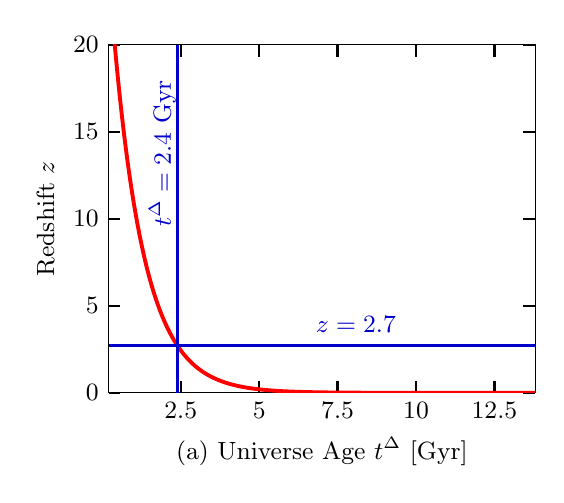
\begin{tikzpicture}
				\begin{axis}[
					width=7cm, height=6cm,
					axis lines = box,
					xlabel = {(a) Universe Age $t^\Delta$ [Gyr]},
					ylabel = {Redshift $z$},
					xmin=0.2, xmax=13.8,
					ymin=0, ymax=20,
					xtick={0.0,2.5,5.0,7.5,10.0,12.5},
					ytick={0,5,10,15,20},
					tick label style={font=\small},
					label style={font=\small},
					smooth,
					every tick/.style={thick, black},
					]
					
					% Redshift curve
					\addplot[color=red, line width=1.4pt, domain=0.2:13.8, samples=300]
					{2.7*exp(-1*(x-2.4))};
					
					% Reference line t = 2.5$\mathrm{Gyr}$
					\draw[blue!80!black, line width=1.0pt] (axis cs:2.4, 0) -- (axis cs:2.4, 20);
					% Reference line z = 2.7
					\draw[blue!80!black, line width=1.0pt] (axis cs:0.2, 2.7) -- (axis cs:13.8, 2.7);
					
					% Text annotations
					\node[blue!80!black, font=\small, anchor=south west, rotate=90] at (axis cs:2.65, 9) {$t^\Delta=2.4\ \mathrm{Gyr}$};
					\node[blue!80!black, font=\small, anchor=south west] at (axis cs:6.5, 2.9) {$z=2.7$};
					
				\end{axis}
			\end{tikzpicture}
		\end{minipage}
		\hfill
		% -------------------- Right panel (b) Refined composite fit --------------------
		\begin{minipage}[b]{0.48\textwidth}
			\centering
			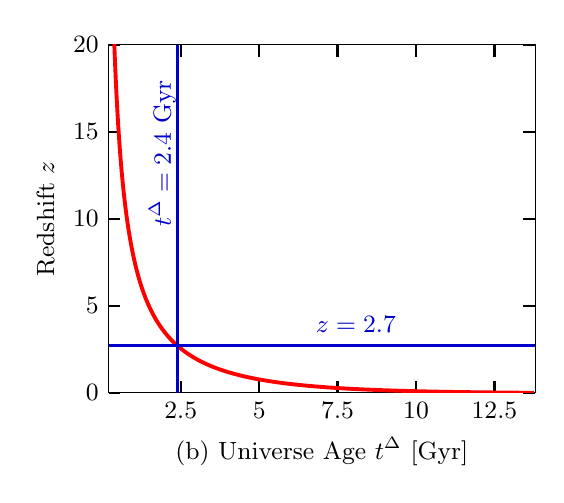
\begin{tikzpicture}
				\begin{axis}[
					width=7cm, height=6cm,
					axis lines = box,
					xlabel = {(b) Universe Age $t^\Delta$ [Gyr]},
					ylabel = {Redshift $z$},
					xmin=0.2, xmax=13.8,
					ymin=0, ymax=20,
					xtick={0.0,2.5,5.0,7.5,10.0,12.5},
					ytick={0,5,10,15,20},
					tick label style={font=\small},
					label style={font=\small},
					smooth,
					every tick/.style={thick, black},
					]
					
					% Refined composite fit curve
					\addplot[color=red, line width=1.4pt, domain=0.2:13.8, samples=300]
					{2.7*exp(-0.16*(x-2.4)) * ((x/2.4)^(-0.84)) * (((13.8-x)/(13.8-2.4))^0.86)};
					
					% Reference line t = 2.4$\mathrm{Gyr}$
					\draw[blue!80!black, line width=1.0pt] (axis cs:2.4, 0) -- (axis cs:2.4, 20);
					% Reference line z = 2.7
					\draw[blue!80!black, line width=1.0pt] (axis cs:0.2, 2.7) -- (axis cs:13.8, 2.7);
					
					% Text annotations
					\node[blue!80!black, font=\small, anchor=south west, rotate=90] at (axis cs:2.65, 9) {$t^\Delta=2.4\ \mathrm{Gyr}$};
					\node[blue!80!black, font=\small, anchor=south west] at (axis cs:6.5, 2.9) {$z=2.7$};
					
				\end{axis}
			\end{tikzpicture}
		\end{minipage}
		
		\vspace{0.1cm}
		
		% Key modification: use footnotesize to make the caption slightly smaller
		\captionsetup{width=0.80\textwidth, font=footnotesize}
		\caption{Redshift $z(t^\Delta)$ profiles using two models:
			(a) Simple exponential model Eq.~(5.3);\enspace \enspace
			(b) improved composite model with exponential, hyperbolic, and pseudo-elliptic components Eq.~(5.6).\enspace \enspace
			Both models are anchored at the reference point $t^\Delta=2.4\ \mathrm{Gyr}$ and $z=2.7$.}
		\label{fig:redshift_fit_comparison}
		
	\end{figure}
	
	
	
	
	
	\medskip
	Both the simple exponential model Eq.~(5.3) and the improved composite model Eq.~(5.6) well reproduce the exponential decay morphology of the observed redshift curve. Meanwhile, the improved model achieves a superior overall fit to $\Lambda$CDM \texttt{Planck18} data across all cosmic epochs.
	\medskip
	
	Nevertheless, we conventionally adopt the simple exponential ansatz $z(t) \propto e^{-t}$ to proceed with our study on time-varying light speed. The relation between $c(t)$, scale factor $a(t)$ and redshift $z(t)$ is given below:
	\medskip
	\[
	\boldsymbol{\frac{c(t)}{c_0}} = \boldsymbol{\frac{a(t)}{a_0}} = \frac{\boldsymbol{1}} {\boldsymbol{1} + \boldsymbol{z(t)}} \,\,,\eqno(5.8)
	\]
	
	\medskip
	We adopt this simple formulation to construct $c(t)$ model for the following reasons:
	\begin{itemize}
		\item It has a compact mathematical formulation and captures the dominant evolutionary trend of cosmic redshift.
		
		\item The cosmic time and expansion history $z(t^\Delta)$ derived from standard $\Lambda$CDM \texttt{Planck18} data are theoretically inferred under the assumption of a constant light speed.
		
		\item To date, no direct observational evidence reveals how the speed of light evolved throughout cosmic history if $c$ is indeed time-dependent.
		
		\item Adopting a time-varying light speed, our theoretical framework is fundamentally distinct from standard cosmology with a constant speed of light.
		
		\item The smooth sigmoid function is a reasonable extrapolation from the redshift $z(t)$ data; its favorable mathematical properties will also facilitate our toy model construction and theoretical analysis.
	\end{itemize}
	\bigskip
	\medskip
	
	
	
	
	{\bf The Growing $\boldsymbol{c(t)}$ Model}\,\,\,
	Our model assumes that the speed of light continuously rises from the early universe to the present day, and will keep increasing slowly in the future. In this framework, we set the cosmic time of the present day to $t = 0$, while earlier cosmic times take larger negative values. This time convention differs from the variable $t^\Delta$ adopted in the preceding redshift model.
	\medskip
	
	Accordingly, we describe the evolving $c(t)$ using a generalized sigmoid function, which features local symmetry about its inflection point:
	\[
	\frac{c(t)}{c_0} = \frac{1}{1 + e^{-k(t+\beta)}} \,\,.\eqno(5.9)
	\]
	
	\medskip
	Here,  $k$ and $\beta$ are two positive parameters to be determined subsequently. In the extremely early universe, as $t \to -\infty$, the exponential term $e^{-k(t+\beta)} \to +\infty$, which means the speed of light back then was far lower than its present value $c_0$.
	
	
	\bigskip
	To normalize the function for the present epoch ($t=0$), where the condition $c(0)/c_0 = 1$ is enforced, a constant factor $(1 + e^{-k\beta})$ is added to the numerator. This yields the final normalized formula:
	\medskip
	\[
	\boldsymbol{C(t)} = \frac{c(t)}{c_0} = \frac{1 + e^{-k\beta}}{1 + e^{-k(t+\beta)}} \,\,.\eqno(5.10)
	\]
	\bigskip
	\medskip
	
	
	{\bf Integral and Derivatives of $\boldsymbol{C(t)}$}\,\,\,
	To evaluate the effective light travel distance across arbitrary cosmic epochs, we first present the definite integral of the normalized light speed function Eq.~(5.10) over a general time interval $[t_1, t_2]$. This integral is essential for comparing our model with observational cosmic timescales.
	\medskip
	
	Introduce a constant to simplify the normalized profile in Eq.~(5.10):
	\[
	J = 1 + e^{-k\beta}\,\,,\eqno(5.11)
	\]
	
	so that
	\[
	\frac{c(t)}{c_0} = \frac{J}{1 + e^{-k(t+\beta)}}\,\,.\eqno(5.12)
	\]
	\medskip
	
	The \textbf{definite integral} over $[t_1, t_2]$ is given by:
	\medskip
	\[
	D(t_1,t_2) = \int_{t_1}^{t_2} \frac{c(t)}{c_0}\,\mathrm{d}t
	= \frac{J}{k}
	\Big[ k(t+\beta) + \ln\big(1+e^{-k(t+\beta)}\big) \Big]
	\Bigg|_{t_1}^{t_2}\,.\eqno(5.13)
	\]
	\medskip
	
	
	We further derive the first and second order derivatives, which describe respectively the variation rate and acceleration of the evolving light speed.
	\medskip
	
	The \textbf{first derivative} (rate of light speed variation) takes the form:
	\medskip
	\[
	\dot{C}(t) = \frac{d}{dt}\left( \frac{c(t)}{c_0} \right)
	=
	\frac{k\,J\,e^{-k(t+\beta)}}
	{\Big(1 + e^{-k(t+\beta)}\Big)^2}\,\,.\eqno(5.14)
	\]
	\medskip
	
	
	For the \textbf{second derivative} (acceleration of light speed variation), we have:
	\medskip
	\[
	\ddot{C}(t) = \frac{d^2}{dt^2}\left( \frac{c(t)}{c_0} \right)
	=
	\frac{k^2\,J\,e^{-k(t+\beta)}\,\Big(e^{-k(t+\beta)} - 1\Big)}
	{\Big(1 + e^{-k(t+\beta)}\Big)^3}\,\,.\eqno(5.15)
	\]
	
	\medskip
	The inflection point denoted as $t_{\text{inf}}$ :
	\[
	t_{\text{inf}} = -\beta\,\,.\eqno(5.16)
	\]
	
	These expressions hold for all admissible positive $k$ and $\beta$. 
	
	
	
	\medskip
	\bigskip
	{\bf The Left Maximum Curvature Point of $\boldsymbol{C(t)}$}\,\,\,
	Referring to the first and second derivatives of $C(t)$ defined in Eq.~(5.14) and Eq.~(5.15) , we now derive the curvature function for the normalized light speed profile.
	\medskip
	
	Following the standard definition of curvature introduced in Eq.~(5.2), the curvature $\kappa(t)$ is always non-negative because its numerator contains an absolute value. Therefore, a point where the first derivative of $\kappa(t)$ equals zero corresponds to a local maximum curvature.
	\medskip
	
	Substituting the derivatives into the curvature formula yields the explicit expression for $\kappa(t)$:
	\medskip
	\[
	\kappa(t) = \frac{\bm{\left|}\ddot{C}(t)\bm{\right|}}{\big[1 + (\dot{C}(t))^2\big]^{3/2}}
	= \frac{
		\bm{\left|}
		\displaystyle
		\frac{k^2 J e^{-k(t+\beta)} \left(e^{-k(t+\beta)} - 1\right)}
		{\left(1 + e^{-k(t+\beta)}\right)^3}
		\bm{\right|}
	}{
		\left[1 + \left(
		\displaystyle
		\frac{k J e^{-k(t+\beta)}}
		{\left(1 + e^{-k(t+\beta)}\right)^2}
		\right)^2\right]^{3/2}
	}\,\,,\eqno(5.17)
	\]
	\medskip
	
	
	Instead of solving this complex expression directly, we resort to an approximate scheme. The parameters $k$ and $J$ slightly break the exact translational invariance of the sigmoid profile, but valid approximate invariance remains satisfied under the condition $kJ\approx 1$. The left maximum curvature point can then be approximated by
	\[
	{t}_{\text{leftmax}} \approx -\beta - \frac{\ln(2+\sqrt{3})}{k}\,\,.\eqno(5.18)
	\]
	
	
	\medskip
	\bigskip
	{\bf Parameter Solving via Cosmic Noon Anchoring}\,\,\,
	Since the genuine evolutionary curve of cosmic light speed cannot be directly observed, we select the most physically meaningful cosmic epoch as the anchor point to solve the parameters $\boldsymbol{k}$ and  $\boldsymbol{\beta}$ in function Eq.~(5.10).
	
	\medskip
	Cosmic Noon corresponds to the epoch of peak cosmic star formation at $t^\star \approx -11.4\ \mathrm{Gyr}$, marking the universe’s evolutionary rhythm at its most vigorous growth stage, coinciding with the curvature maximum of the model’s evolutionary curve, and serving as the most representative temporal anchor point.
	
	\medskip
	Denoting the cosmic noon time by $\boldsymbol{t_w}$, we impose three independent physical constraints:
	\begin{itemize}
		\item The effective light-travel integral from Eq.~(5.13) satisfies $D(t_w,0)=11.4$$\mathrm{Gyr}$, equal to the integrated light propagation distance spanning cosmic noon to the present day.
		
		\item The normalized light speed at cosmic noon reads $C(t_w)=1/3.7$, constrained by the measured redshift $z=2.7$ together with the model definition in Eq.~(5.10).
		
		\item Based on physical self-consistency, cosmic noon coincides with the left curvature maximum from Eq.~(5.18), i.e., $t_w = t_{\text{leftmax}}$, where the acceleration change rate of $c(t)$ reaches its peak.
	\end{itemize}
	
	\medskip
	These three constraints form a closed algebraic system for the three unknown variables $\boldsymbol{k}$, $\boldsymbol{\beta}$ and $\boldsymbol{t_w}$, explicitly written as
	\[
	\left\{
	\begin{aligned}
		\displaystyle \quad \frac{J}{k}\Big[ k(t+\beta) + \ln\big(1+e^{-k(t+\beta)}\big) \Big]\Bigg|_{t_w}^{0} \enspace &= \enspace 11.4\\[6pt]
		\displaystyle \quad \frac{1 + e^{-k\beta}}{1 + e^{-k(t_w+\beta)}} \enspace &= \enspace \frac{1}{3.7}\\[6pt]
		\displaystyle \quad -\beta - \frac{\ln(2+\sqrt{3})}{k} \enspace &= \enspace t_w 
	\end{aligned}
	\right.\eqno(5.19)
	\]
	
	
	
	The resulting parameters read
	\[
	\boldsymbol{k} = 0.1442, \quad \boldsymbol{\beta} = 8.854, \quad \boldsymbol{t_w} = -17.98\,\mathrm{Gyr}, \quad \boldsymbol{J} = 1.2789. \eqno(5.20)
	\]
	
	\medskip
	Up to this point, the compact growing-$c(t)$ model has been fully established. Detailed physical interpretation will be discussed in the following sections.
	
	\bigskip
	\noindent
	$\triangleright \triangleright \triangleright$\enspace
	For the equations system listed in Eq.~(5.19), multiplying the right-hand-side value $11.4$ of the integral constraint $D(t_w,0)$ by $1.25$ (yielding $14.25$) and scaling the denominator constant $3.7$ in the light-speed relation $C(t_w)$ also by the same factor $1.25$ (yielding $4.625$) leads to an alternative set of solved parameters:
	\[
	\boldsymbol{k} = 0.2550, \quad \boldsymbol{\beta} = 14.77, \quad \boldsymbol{t_w} = -19.93\,\mathrm{Gyr}, \quad \boldsymbol{J} = 1.0231. \eqno(5.21)
	\]
	
	When adopting this parameter-modified model, within the time range $t\in[-60,5]$, which corresponds to cosmic window from ancient $-60\ \mathrm{Gyr}$ to $5\ \mathrm{Gyr}$ in the future, the resulting $C(t)$ profile exhibits an ideal, nearly perfect sigmoid shape. The physical origin of this scaling factor $1.25$ remains unclarified, or it may merely arise from accidental coincidence, and relevant discussion is open to the academic community.\enspace$\triangleleft \triangleleft \triangleleft$
	
	\bigskip
	\textit{\textbf{Note:} One may construct a variant of the growing-$c(t)$ model by defining the function via the improved composite model in Eq.~(5.6); however, this formulation features an overly intricate mathematical structure and thus lies beyond the scope of the present work.}
	
	
	
	
	
	
	\section*{
		\begin{center}
			6. Ultra-fine Growing-$\boldsymbol{c(t)}$ Model
		\end{center}
	}
	\medskip
	\noindent
	
	In the standard $\Lambda$CDM cosmology, only cosmic redshifts can be directly observed. Precise cosmic expansion history and corresponding cosmic time are unmeasurable in practice.
	
	\medskip
	All cosmic time entries stored in the \texttt{Planck18} dataset are model-derived quantities. Such calculations rely on three fundamental premises: \textit{homogeneous and isotropic universe}, \textit{invariant total matter and energy}, and \textit{constant speed of light}. Cosmic ages are further solved via the Friedmann equations under these restrictions.
	
	\medskip
	Under our $G(t)\,c(t)^2 = P$ postulate, $G(t)$ is time-varying, which implies that the stellar mass estimation methods used in $\Lambda$CDM contain inherent biases. A detailed discussion of this issue is deferred to Section 12.
	
	\medskip
	Despite being constrained by preset theoretical assumptions and the inevitable uncertainties in model derivation, the \texttt{Planck18} data still stands as the best available reference. We therefore construct our ultra-fine growing-$c(t)$ model grounded on this dataset.
	
	
	
	\medskip
	\bigskip
	{\bf Data Extraction}\,\,\,
	The \texttt{Planck18} standard redshift–cosmic time dataset $(z,\, {t}^\vartriangle)$ is extracted from the Python \texttt{astropy.cosmology} library at float64 numerical precision.
	
	
	\medskip
	The total cosmic age is approximately $13.8\ \mathrm{Gyr}$. We partition the full cosmic timeline with a fixed timestep of $10^4$ years (10 kyr) for uniform sampling. This yields roughly $13.8\times10^{5}$ sampled data points.
	
	\medskip
	Sampling begins at the present cosmic time ${t}^\vartriangle=13.79069_{\boldsymbol\cdots}\mathrm{Gyr}$, with each subsequent sample reduced by $10^4$ years: the second and third sampled times equal ${t}^\vartriangle=13.79068_{\boldsymbol\cdots}$ and ${t}^\vartriangle=13.79067_{\boldsymbol\cdots}$, respectively.
	
	\medskip
	The redshift of CMB epoch is $z\simeq 1090$, which defines the uppermost observational boundary. For this reason, sampling is truncated at ${t}^\vartriangle=0.00037_{\boldsymbol\cdots}$ and ${t}^\vartriangle=0.00036_{\boldsymbol\cdots}$, corresponding to $z=1083.07$ and $z=1100.61$, namely 37 kyr and 36 kyr after the Big Bang, in line with this physical limit.
	
	\medskip
	In total, $N=1\,379\,024$ equal-time-interval raw time-redshift pairs are extracted.
	\medskip
	
	
	\bigskip
	{\bf Definition of Interval Distance $\boldsymbol{yr_i}$}\,\,\,
	Following the piecewise averaging rule, the segment time distance for each time interval is defined as
	$$
	\mathit{yr}_i=1+\frac12\left(z_i+z_{i+1}\right) \,\,,\eqno(6.1)
	$$
	
	where $i\in (0,\,1379022)$, and $z_i$ denotes the redshift at the $i$-th sampling point. All $yr_i$ values are computed sequentially over the full valid intervals.
	
	\medskip
	Each piecewise $yr_i$ stands for the time scaling factor derived under the growing-$c(t)$ model. For example, $yr_i=1.5$ corresponds to an averaged redshift $\bar z=0.5$ from $z_i$ and $z_{i+1}$; the original $10^4$ years of sampling interval is scaled to $1.5\times 10^4$ years within the growing-$c(t)$ framework.
	\medskip
	
	
	
	\bigskip
	{\bf Cumulative Summation $\boldsymbol{\mathrm{YR}_i}$}\,\,\,
	We accumulate the sequence $yr_i$ following Eq.~(6.2) to compute the total cosmic timescale under the growing-$c(t)$ model. To suppress floating-point round-off error arising from millions of successive additions, the Kahan summation algorithm is adopted for residual error compensation.
	\[
	\mathrm{YR}_i = \mathrm{YR}_{i-1} + yr_i \,\,,\quad \mathrm{YR}_0 = yr_0 \,\,.\eqno(6.2)
	\]
	
	The resulting $\mathrm{YR}_i$ array represents the growing-$c(t)$ timescale quantified in units of $10^4$ years. Each $\mathrm{YR}_i$ is multiplied by $-1$ to denote negative cosmic time. The formation point of the CMB epoch corresponds to $-45.2\ \mathrm{Gyr}$.
	\medskip
	
	
	\bigskip
	{\bf $\boldsymbol{C(t)}$ Normalizing and $\boldsymbol{\mathrm{YR}_i}$ Downsampling}\,\,\,
	The normalized $C(t)$ follows $C(t) = 1/(1+z_t)$ from sampled redshift sequences, which produces full-resolution $C(t)$ data with $1\,379\,023$ entries.
	
	\medskip
	For convenient presentation within this work, we perform downsampling by retaining one datum per 1000 raw samples. This procedure yields 1381 discrete sets of growing-$c(t)$ and corresponding time $\mathrm{YR}_i$, with an effective spacing of $t^\Delta = 10^7\ \mathrm{years}$ between neighboring data. 
	
	\medskip
	This dataset serves as the core database for the proposed ultra-fine growing-$c(t)$ model. Its corresponding curve is presented in following figure.
	\bigskip
	
	\begin{figure}[H]
		\centering
		\begin{tikzpicture}
			\begin{axis}[
				width=14cm, height=8cm,
				axis lines = box,
				xlabel = {Cosmic Time \(t\) [Gyr]},
				ylabel = {growing-\(c(t)\)},
				xmin=-50, xmax=5,
				ymin=0.0, ymax=1.2,
				xtick = {-50, -45, -40, -35, -30, -25, -20, -15, -10, -5, 0, 5},
				ytick = {0.0, 0.2, 0.4, 0.6, 0.8, 1.0, 1.2},
				tick label style={font=\small},
				label style={font=\small},
				every tick/.style={thick, black},
				]
				
				% Read your 1381 sets of measured data, red small squares, no connecting lines
				\addplot[
				color=red,
				only marks,
				mark=square,
				mark size=0.8pt,
				] table [col sep=comma, x=X, y=Y] {2026-growing-ct-fine-model-1381.csv};
				
				
				% Reference line z_3 = Solar System, -5.57Gyr, 0.70 
				\draw[blue!80!black, line width=1.0pt] (axis cs:-5.57, 0) -- (axis cs:-5.57, 1.2);
				\draw[blue!80!black, line width=0.4pt] (axis cs:-60, 0.70) -- (axis cs:-3, 0.70);
				% Text annotation
				\node[blue!80!black, font=\small, anchor=south west, rotate=90] at (axis cs:-5.68, 0.50) {${z_3}$\,\,\,Solar-System};
				
				% Reference line z_1 = Early Galaxy, -36.8Gyr, 0.04 
				\draw[blue!80!black, line width=1.0pt] (axis cs:-20, 0) -- (axis cs:-20, 1.2);
				\draw[blue!80!black, line width=0.4pt] (axis cs:-60, 0.27) -- (axis cs:-16, 0.27);
				% Text annotation
				\node[blue!80!black, font=\small, anchor=south west, rotate=90] at (axis cs:-20.1, 0.29) {${z_2}$\,\,\,Cosmic-Noon};
				
				% Reference line z_1 = Early Galaxy, -36.8Gyr, 0.04 
				\draw[blue!80!black, line width=1.0pt] (axis cs:-36.8, 0) -- (axis cs:-36.8, 1.2);
				\draw[blue!80!black, line width=0.4pt] (axis cs:-60, 0.04) -- (axis cs:-32, 0.04);
				% Text annotation
				\node[blue!80!black, font=\small, anchor=south west, rotate=90] at (axis cs:-36.9, 0.13) {${z_1}$\,\,\,Early-Galaxy};
				
				% Reference line z_0 = CMB Decoupling, -45.2Gyr, 0.092%
				\draw[blue!80!black, line width=1.0pt] (axis cs:-45.2, 0) -- (axis cs:-45.2, 1.2);
				% Text annotation
				\node[blue!80!black, font=\small, anchor=south west, rotate=90] at (axis cs:-45.3, 0.03) {${z_0}$\,\,\,CMB-Decoupling};
				
			\end{axis}
		\end{tikzpicture}
		
		\vspace{0.2cm}
		\captionsetup{width=0.85\textwidth, font=footnotesize}
		\caption{
			The $\mathrm{C(t)}$ curve of the ultra-fine growing-$c(t)$ model, derived from \texttt{Planck18} data.
			The corresponding cosmic times of the four benchmark epochs $z_0, z_1, z_2, z_3$ will be explained in the following section.}
		\label{fig:growing_ct_fine_model}
		
	\end{figure}
	
	
	
	
	
	
	\section*{
		\begin{center}
			7. Different Physical Pictures of \\
			Growing-\(\boldsymbol{c(t)}\) Universe
		\end{center}
	}
	\medskip
	\noindent
	
	This section depicts an extensive set of dramatically different physical pictures of cosmic evolution across various cosmic epochs. 
	
	\medskip
	The cosmic origin timescale is extended to $[-59.1,\,-45.2]\,$$\mathrm{Gyr}$, while at the CMB decoupling epoch, the light speed \(c(t)\) equals \(1/1100\) of the present speed \(c_0\), the Bohr radius \(a_\text{B}\) is only \(1/1100\) of its present value, and the ionization temperature of hydrogen atoms ${T_\mathrm{ion}(t)}$ amounts to merely 82.64$\,\mathrm{K}$. 
	
	\medskip
	Many physical quantities from the classical basic equations evolve alongside \(c(t)\), and separate subsections will elaborate each topic sequentially.
	
	\medskip
	All present-day values of fundamental physical constants used in this work (e.g., the Bohr radius $a_{\scriptscriptstyle\mathrm{B},0}$, the reduced Planck constant $\hbar_0$, and the proton diameter $d_p$) are taken from standard reference sources\cite{Tipler:2008}.
	
	\bigskip
	{\bf Cosmic Origin Timescale}\,\,\,
	The CMB decoupling epoch marks the origin point of the observable universe, corresponding to a redshift satisfying $1+z=1100$. 
	
	\medskip
	Under the compact growing-$c(t)$ model defined in Eq.~(5.10), $C(t)=1/1100$ yields $t=-59.1\,\mathrm{Gyr}$; for the ultra-fine growing-$c(t)$ model, the cosmic time reads $t=-45.2\,\mathrm{Gyr}$ at the early CMB stage with redshift $z=1083.07$. These results imply a gently evolving cosmos rather than a violent Big Bang scenario\cite{Weinberg:2008}. 
	
	\medskip
	A preliminary assessment shows that the time span between the QGP threshold epoch ($\boldsymbol{z_{\star}}$) and the CMB decoupling epoch ($\boldsymbol{z_{1}}$) surpasses the 36-37\,$\mathrm{kyr}$ given by the standard $\Lambda$CDM model.
	
	\medskip
	The ultimate cosmic origin was postulated as the \textit{Zero-Light-Speed Zero-Temperature} (\textit{ZLZT}) primordial state, where both the speed of light and temperature approach zero. We infer that if the cosmic speed of light falls below  42\,$\mathrm{km/s}$ (21$\,\mathrm{km/s}$ or \allowbreak 14 $\mathrm{km/s}$) and the ambient temperature stays near 2.75$\,\mathrm{K}$ at the QGP threshold epoch ($\boldsymbol{z_{\star}}$), all hadronic structures fully dissociate into free quarks and gluons, forming a pure quark–gluon universe without hadrons. Detailed discussions are given in Section 9.
	
	
	\bigskip
	{\bf Cosmic Noon and  $\boldsymbol{C(t)}$}\,\,\,
	Based on the compact growing-$c(t)$ model from Eq.~(5.20), Cosmic Noon occurs at $t_w = -17.98\,\mathrm{Gyr}$. For the ultra-fine growing-$c(t)$ model described in Eq.~(6.2), this epoch falls at $t_w = -20.21\,\mathrm{Gyr}$. Both timestamps differ substantially from $t^\star = -11.4\,\mathrm{Gyr}$ predicted by the standard $\Lambda$CDM model. 
		
	\medskip
	At Cosmic Noon, the cosmic light speed reaches $27.03\%$ of the present value $c_0$, equivalent to $1/3.7\,c_0$. Per the scaling relation $r_s \propto c^{-4}$ derived in Eq.~(1.11), the Schwarzschild radius at this epoch was $3.7^4 = 187.4$ times larger than its present-day counterpart, which explains the efficient formation of black holes in this cosmic era.

		
	\bigskip
	{\bf Solar System Formation}\,\,\,
	For the epoch of Solar System formation ($\boldsymbol{z_3}$), the \texttt{Planck18} dataset gives $t^\star = -4.67\,\mathrm{Gyr}$ at redshift $z=0.43$. 
	
	\medskip
	The compact and ultra-fine growing-$c(t)$ model yield $-7.55\,\mathrm{Gyr}$ and $-5.57\,\mathrm{Gyr}$, respectively. We consider the latter result more reliable, since the ultra-fine model is calibrated using the full \texttt{Planck18} dataset, whereas the compact model relies on only a single data point. The relative light speed at this epoch is $69.93\%$. 
	
	\medskip
	Data for the early galaxy formation epoch ($\boldsymbol{z_1}$) are summarized in the table below and will not be discussed further.
	
	\bigskip
	\begin{table}[H]
		\centering
		\captionsetup{skip=2pt, font=small}
		\caption{$\boldsymbol{C(t)}$ and $\boldsymbol{t}$ of benchmark epochs $\boldsymbol{z_i}$}
		\footnotesize
		\renewcommand{\arraystretch}{1.50}
		\begin{tabular}{>{\centering\arraybackslash}p{2.5cm}|>{\centering\arraybackslash}p{2cm}>{\centering\arraybackslash}p{2cm}|>{\centering\arraybackslash}p{2cm}>{\centering\arraybackslash}p{2cm}}
			\toprule
			\textbf{Parameter} & \textbf{$\boldsymbol{z_0}$} & \textbf{$\boldsymbol{z_1}$} & \textbf{$\boldsymbol{z_2}$} & \textbf{$\boldsymbol{z_3}$} \\
			\midrule
			$\boldsymbol{C(t)}$                     & $1/1100$    & $1/25$    & $1/3.7$   & $1/1.43$   \\
			$\boldsymbol{C(t)\,\,\%}$               & $0.09\%$    & $4.00\%$  & $27.03\%$ & $69.93\%$  \\
			$\boldsymbol{t}\mathsf{_{compact}}$     & $-59.1$     & $-32.7$   & $-17.83$  & $-7.55$    \\
			$\boldsymbol{t}\mathsf{_{fine}}$        & $-45.2$     & $-36.6$   & $-20.21$  & $-5.57$    \\
			$\boldsymbol{t^\star}$                  & $-13.8$     & $-13.6$   & $-11.40$  & $-4.67$    \\
			\bottomrule
		\end{tabular}
	\end{table}
	
	
	
	\medskip
	{\bf Dimensional Analysis}\,\,\,
	Physics defines seven fundamental dimensional quantities, abbreviated as \texttt{LMTI$\Theta$NJ}. They stand for length (\texttt{L}), mass (\texttt{M}), time (\texttt{T}), electric current (\texttt{I}), thermodynamic temperature (\texttt{$\Theta$}), amount of substance (\texttt{N}) and luminous intensity (\texttt{J}), respectively.
	
	\medskip
	This paper is built upon two core postulates listed in Section 2. The macroscopic postulate is given by ${G(t)}\tinysp {c(t)^2} = \boldsymbol{P}$, which indicates $G(t) \propto c(t)^{-2}$. The microscopic postulate states that the fine-structure constant $\boldsymbol{\alpha}$ is universally invariant throughout cosmic evolution.
	
	\medskip
	Based on these postulates, a subset of the physical quantities from Section 1 evolve with $c(t)$. We derive their dimensions and power-law relations with $c(t)$, as summarized in the table below.
	
	\medskip
	\begin{table}[H]
		\centering
		\captionsetup{skip=2pt, font=small}
		\caption{Dimensional analysis and power-law scaling with $\boldsymbol{c(t)}$}
		\footnotesize
		\renewcommand{\arraystretch}{1.50}
		\begin{tabular}{>{\centering\arraybackslash}p{2.5cm}|>{\hspace{0.5cm}\raggedright\arraybackslash}p{4.2cm}|>{\hspace{0.5cm}\centering\arraybackslash}p{5.5cm}}
			\toprule
			\textbf{Evolving Qty.} & \textbf{Dimensional Form} & \textbf{Power-law Scaling with $\boldsymbol{c(t)}$} \\
			\midrule
			$G(t)$                                  & $[G]$ : $\mathrm{L}^{3}\, \mathrm{M}^{-1}\, \mathrm{T}^{-2}$                                & ${\propto c^{-2}}$ \\
			$\mu_0(t)$                              & $[\mu_0]$ : $\mathrm{L}^{1}\, \mathrm{M}\, \mathrm{T}^{-2}\, \mathrm{I}^{-2}$               & ${\propto c^{+1}}$ \\
			$\varepsilon_0(t)$                      & $[\varepsilon_0]$ : $\mathrm{L}^{-3}\, \mathrm{M}^{-1}\, \mathrm{T}^{4}\, \mathrm{I}^{2}$   & ${\propto c^{-3}}$ \\
			$\hbar(t)$                              & $[\hbar]$ : $\mathrm{L}^{2}\, \mathrm{M}\, \mathrm{T}^{-1}$                                 & ${\propto c^{+2}}$ \\
			$a_{\scriptscriptstyle\mathrm{B}}(t)$   & $[a_{\mathrm{B}}]$ : $\mathrm{L}^{1}$                                                       & ${\propto c^{+1}}$ \\
			$k_e(t)$                                & $[k_e]$ : $\mathrm{L}^{3}\mathrm{M}\, \mathrm{T}^{-4}\, \mathrm{I}^{-2}$                    & ${\propto c^{+3}}$ \\
			\bottomrule
		\end{tabular}
	\end{table}
	
	\medskip
	The remaining six quantities are derived from the foregoing results. Their dimensional forms and power-law scaling with $c(t)$ are presented in the following table.
	
	\medskip
	\begin{table}[H]
		\centering
		\captionsetup{skip=2pt, font=small}
		\caption{Power-law scaling of the remaining four quantities with $\boldsymbol{c(t)}$}
		\footnotesize
		\renewcommand{\arraystretch}{1.50}
		\begin{tabular}{>{\centering\arraybackslash}p{2.5cm}|>{\centering\arraybackslash}p{1.8cm}|>{\hspace{0.5cm}\raggedright\arraybackslash}p{8.2cm}}
			\toprule
			\textbf{Evolving Qty.} & \textbf{Ref. Eq.} & \textbf{Power-law Scaling with $\boldsymbol{c(t)}$} \\
			\midrule
			$m_{\scriptscriptstyle\mathrm{P}}(t)$    &$\mathrm{Eq.}(1.3)$      & ${\hbar \propto c^{+2}},\enspace {c^{+1}\propto c^{+1}},\enspace {G^{-1}\propto c^{+2}}  \quad \Rightarrow \quad {\propto \boldsymbol{c^{\frac{5}{2}}}  }$  \\
			$\ell_{\scriptscriptstyle\mathrm{P}}(t)$ &$\mathrm{Eq.}(1.4)$      & ${\hbar \propto c^{+2}},\enspace {c^{-3}\propto c^{-3}},\enspace {G^{+1}\propto c^{-2}}  \quad \Rightarrow \quad {\propto \boldsymbol{c^{-\frac{3}{2}}} }$  \\
			$\rho_{\scriptscriptstyle\mathrm{P}}(t)$ &$\mathrm{Eq.}(1.5)$      & ${\hbar^{-1} \propto c^{-2}},\enspace {c^{+5} \propto c^{+5}},\enspace {G^{-2} \propto c^{+4}} \Rightarrow \quad {\propto \boldsymbol{c^{7}}      }$        \\
			$T_{\mathrm{ion}}(t)$  &$\mathrm{Eq.}(1.8)$    & ${\Rightarrow \quad {\propto \boldsymbol{c^{2}}}}     $  \\
			$r_{\mathrm{s}}(t)$ &$\mathrm{Eq.}(1.11)$      & ${\Rightarrow \quad {\propto \boldsymbol{c^{-4}}}}    $  \\
			$N_{\mathrm{Dirac}}(t)$ &$\mathrm{Eq.}(1.16)$    & $ {G \propto c^{-2}},\enspace \varepsilon_0 \propto c^{-3} \Rightarrow \quad {\propto \boldsymbol{c^{5}}      }$        \\
			\bottomrule
		\end{tabular}
	\end{table}
	
	
	\medskip
	\textbf{Evolution of $\boldsymbol{\varepsilon_0(t)}$, $\boldsymbol{\mu_0(t)}$}\,\,\,
	$\varepsilon_0(t)$ and $\mu_0(t)$ are the core quantities governing the evolution of $c(t)$. Following $\varepsilon_0(t) \propto c(t)^{-3}$ and $\mu_0(t) \propto c(t)$, the two parameters decrease and increase respectively as $c(t)$ rises and mutually constrain one another, in accordance with the core form of Maxwell's equations, as shown in Eq.~(7.1). 
	\[
	\mu_0(t)\,\varepsilon_0(t)\, c(t)^2 = 1\,\,. \eqno(7.1)
	\]
	
	\medskip
	The three quantities $\mu_0(t)$, $\varepsilon_0(t)$ and $c(t)$ are governed by the \textit{Light-Electricity-Magnetism} \textit{Synchronized Cosmic Dark Field} (\textit{LEM-SCDF}), which will be fully elaborated in subsequent sections.
	
	
	\medskip
	\bigskip
	\textbf{Evolution of the Bohr Radius $\boldsymbol{a_{\scriptscriptstyle\mathrm{B}}(t)}$}\,\,\,
	In our framework, the Bohr radius $a_{\scriptscriptstyle\mathrm{B}}(t)$ of hydrogen scales linearly with $c(t)$, in contrast to the conventional assumption of a constant. At the epoch $1+z=25$, its value equals $1/25$ of the present-day value. At the CMB epoch with $1+z=1100$, the Bohr radius is reduced to $1/1100$ of its current magnitude.
	
	\medskip
	The present-day Bohr radius is $a_{\scriptscriptstyle\mathrm{B},0}=5.292\times10^{-11}\,\mathrm{m}$, and the proton diameter is $d_p=1.6815\times10^{-15}\,\mathrm{m}$. Their present-day ratio is approximately $3.15\times10^4$. At $1+z=1100$, the ratio drops to roughly $28.6$, indicating an extremely narrow electron orbit around the proton in the early universe. This ratio represents the bare minimum scale to sustain neutral hydrogen. Before the cosmic evolution reached this stage, the orbital radius was too small to form stable hydrogen atoms.
	
	\medskip
	This scenario has rarely been investigated in existing studies. When the Bohr radius was merely dozens of times the proton diameter, multi-electron atoms and complex molecular bonds could hardly form, as electron shells were compressed into overlapping configurations. Additionally, the transition from plasma to neutral hydrogen during recombination was fragile and reversible; newly formed atoms were loosely bound and likely to be reionized.
	
	\medskip
	The orbital scale of atoms further governs the abundance of chemical elements. In the era near CMB, the severely compacted atomic structure would have permitted only hydrogen-dominated objects to condense, with almost no complex heavy elements. Simple chemical compositions remained prevalent for a long time in the early cosmic environment.
	
	
	\medskip
	\bigskip
	\textbf{Evolution of Coulomb parameter $\boldsymbol{k_e(t)}$}\,\,\,
	As analyzed in Table 3, the Coulomb parameter $k_e(t)$ scales with the cube of cosmic light speed $c(t)$. At redshift $1+z=25$, $k_e(t)$ is $1/25^3$ of its present value, while at the CMB epoch ($1+z=1100$), it reduces to $1/1100^3$ of the current magnitude. The drastically weakened electrostatic force in the early universe led to fragile atomic bonding at the microscopic scale, consistent with the evolutionary characteristics of hydrogen atoms discussed above.
	
	
	\medskip
	\bigskip
	\textbf{Evolution of Planck Quantities $\boldsymbol{\hbar(t)}$, $\boldsymbol{m_{\scriptscriptstyle\mathrm{P}}(t)}$, $\boldsymbol{\ell_{\scriptscriptstyle\mathrm{P}}(t)}$ and $\boldsymbol{\rho_{\scriptscriptstyle\mathrm{P}}(t)}$}\,\,\,
	As analyzed in Table 3 and Table 4, the reduced Planck constant $\hbar(t) \propto c(t)^{2}$, the Planck mass $m_{\scriptscriptstyle\mathrm{P}}(t) \propto c(t)^{5/2}$, the Planck length $\ell_{\scriptscriptstyle\mathrm{P}}(t)\propto c(t)^{-3/2}$, and the conventional Planck density $\rho_{\scriptscriptstyle\mathrm{P}}(t)$ evolves proportionally to $c(t)^7$.
	
	\medskip
	In the present-day universe, the Planck mass reaches $m_{\scriptscriptstyle\mathrm{P,0}} \approx 2.2\times 10^{-8}\,\mathrm{kg} \approx 22\, \mathrm{\mu g}$, which is extremely massive for a microscopic scale, while the Planck length $\ell_{\scriptscriptstyle\mathrm{P},0} \approx 1.6\times 10^{-35}\,\mathrm{m}$ remains extraordinarily tiny, and the Planck density $\rho_{\scriptscriptstyle\mathrm{P},0} \approx 5.2\times 10^{96}\,\mathrm{kg/m^3}$.
	
	\medskip
	Since $\rho_{\scriptscriptstyle\mathrm{P}}(t) \propto c(t)^7$, at the CMB epoch (${z_0}$) with $1+z=1100$, we have $1100^7 \approx 1.95 \times 10^{21}$. This reduces the Planck density to $\rho_{\scriptscriptstyle\mathrm{P}}(t) \approx 2.65\times 10^{75}\,\mathrm{kg/m^3}$. 
	
	\medskip
	Furthermore, at the post-hadronization plasma epoch (${z_{\star}}$), the speed of light drops to 1/7137.66 of its present-day value $c_0$, i.e., approximately 42 km/s. We get $7137.66^7 \approx 9.44 \times 10^{26}$. This reduces the Planck density to $\rho_{\scriptscriptstyle\mathrm{P}}(t) \approx 5.51\times 10^{69}\,\mathrm{kg/m^3}$.
		
	\medskip
	Both Planck densities above are far greater than the Friedmann cosmic density $\rho_{\scriptscriptstyle\mathrm{F}}(t)$ defined in Eq.~(1.14). We will revisit these quantities when we discuss ${v_{\scriptscriptstyle\mathrm{LEM}}(t)}$ in Eq.~(8.6) later, where both $\rho_{\scriptscriptstyle\mathrm{P}}(t)$ and $\rho_{\scriptscriptstyle\mathrm{F}}(t)$ will be used.
	
	\medskip
	If we eliminate $G$ and replace it with $P = Gc^2$, the three Planck quantities in Eq.~(1.3), Eq.~(1.4), and Eq.~(1.5) become:
	\[
	m_P(t) = \sqrt{\frac{\hbar(t) \cdot c(t)^3}{P}}, \quad \ell_P(t) = \sqrt{\frac{\hbar(t) \cdot P}{c(t)^5}}, \quad \rho_P(t) = \frac{c(t)^9}{\hbar(t) \cdot P^2}\,\,. \eqno(7.2)
	\]
	
	
	\medskip
	\bigskip
	\textbf{Evolution of Boltzmann Ionization Criterion  $\boldsymbol{T_\mathrm{ion}(t)}$}\,\,\,
	As analyzed in Table 4, the ionization temperature of hydrogen atoms scales with the cosmic speed of light, following ${T_\mathrm{ion}}(t) \propto c(t)^2$. The present-day ${T_\mathrm{ion}}(t)$ is approximately $10^8\,\mathrm{K}$, and the values of ${T_\mathrm{ion}}(t)$ at four typical cosmic epochs are given in Table 5.
	
	\begin{table}[H]
		\centering
		\captionsetup{skip=2pt, font=small}
		\caption{Ionization temperature $\boldsymbol{T_\mathrm{ion}}$ at benchmark epochs $\boldsymbol{z_i}$}
		\footnotesize
		\renewcommand{\arraystretch}{1.50}
		\begin{tabular}{>{\centering\arraybackslash}p{2.5cm}|>{\centering\arraybackslash}p{2cm}>{\centering\arraybackslash}p{2cm}>{\centering\arraybackslash}p{2cm}>{\centering\arraybackslash}p{2cm}}
			\toprule
			\textbf{Parameter} & \textbf{$\boldsymbol{z_0}$} & \textbf{$\boldsymbol{z_1}$} & \textbf{$\boldsymbol{z_2}$} & \textbf{$\boldsymbol{z_3}$} \\
			\midrule
			$\boldsymbol{C(t)}$      & $1/1100$   & $1/25$    & $1/3.7$   & $1/1.43$  \\
			$\boldsymbol{T_\mathrm{ion}\,(\mathrm{K})}$  & $>82.64$ & $>1.60\times10^{5}$ & $>7.31\times10^{6}$ & $>4.89\times10^{7}$ \\
			\bottomrule
		\end{tabular}
		\label{tab:ion_temp}
	\end{table}
	
	According to the Boltzmann formula Eq.~(1.8), if the cosmic speed of light drops to \(1/7137.66\) of its present value, corresponding to $c(t)=42.03\,\mathrm{km/s}$, the ionization temperature reduces to \(1.96\,\mathrm{K}\). In other words, at this light speed, any temperature exceeding \(1.96\,\mathrm{K}\) is sufficient to dissociate neutral hydrogen atoms into plasma.
	
	\medskip
	As will be further discussed in Section 9, raising the temperature from \(1.96\,\mathrm{K}\) to \(2.75\,\mathrm{K}\) induces quark deconfinement and hadron dissociation, transforming the plasma into a sea of free quarks and gluons. We will also conduct a detailed analysis of this phenomenon, alongside research on the initial Zero-Light-Speed and Zero-Temperature (ZLZT) cosmic state, in the same section.
	
	
	\medskip
	\bigskip
	\textbf{Evolution of Schwarzschild Radius $\boldsymbol{r_s(t)}$}\,\,\,
	As analyzed in Table 4, the radius defined in Eq.~(1.11) scales as $r_s(t) \propto c(t)^{-4}$. At high redshift epochs $1+z=25$ and $1+z=7$, $r_s(t)$ is $25^4 = 390{,}625$ and $7^4 = 2{,}401$ times its present-day value, respectively. At Cosmic Noon $1+z=3.7$, the radius was $3.7^4 \approx 187.4$ times larger than today.
	
	\medskip
	This large increase of $r_s(t)$ in the early universe had strong effects on how structures formed. With a much larger gravitational reach, early stars and compact objects could easily pull in nearby matter. As a result, they quickly cleared away the material around them, leaving little chance for planets to form. At the same time, the stronger gravity squeezed these stars more tightly, making them burn their fuel faster and evolve more quickly. This gives a new way to understand why the earliest galaxies seem to contain mostly stars, with few signs of planetary systems — a point that has not been discussed before in this context.
	
	\medskip
	As cosmic $c(t)$ continues to grow toward its present value, $r_s(t)$ shrinks steadily, following $c(t)^{-4}$. This weakening of gravitational influence means that later stars are much less able to capture surrounding material. By the time the Solar System formed at $1+z \approx 1.43$, $r_s(t)$ had already dropped to about $(1.43/3.7)^4 = 22.3\%$ of its value at Cosmic Noon. The early universe was thus a place of strong gravitational activity, which gradually calmed down over time, allowing quieter planetary systems like our own to form in later epochs.
	
	\medskip
	A natural extension of this picture would be to quantify the suppression of planet formation as a function of redshift. One may heuristically write
	\[
	P_{\rm planet}(z) \; \propto \; \left(\frac{r_s(z)}{r_{\rm disk}(z)}\right)^{-\beta} \propto \; (1+z)^{4\beta},\,\, \eqno(7.3)
	\]
	
	where $r_{\rm disk}(z)$ is the characteristic scale of a protoplanetary disk and $\beta>0$ is a phenomenological index. A more rigorous derivation could be attempted from gravitational focusing or Bondi accretion physics, relating the enhanced capture cross-section to the likelihood of disk survival and subsequent planet assembly.
	 
	\medskip
	However, such a quantitative treatment lies beyond the scope of the present work. We include this expression solely as a heuristic indication of how the growing-$c(t)$ framework might lead to testable predictions for the redshift dependence of planetary system formation, should future observational data become available.
	
	
	\medskip
	\bigskip
	\textbf{Evolution of the Dirac Large Number $\boldsymbol{N_{\mathrm{Dirac}}(t)}$}\,\,\,
	As analyzed in Table 4, the Dirac larger ratio~\cite{Dirac:1937} in Eq.~(1.16) scales as $N_{\mathrm{Dirac}}(t) \propto c(t)^{5}$. The present‑day ratio is $\approx 2.26 \times 10^{39}$. At the CMB epoch with $1+z=1100$, the large number is reduced to $(1/1100)^5$ of its current value, yielding $N_{\mathrm{Dirac,CMB}} \approx 1.40\times 10^{24}$.
	
	\medskip
	Notice that such a dramatic reduction of the electromagnetic‑to‑gravitational force ratio at the CMB epoch is a distinctive prediction of our varying‑speed‑of‑light framework. A smaller $N_{\mathrm{Dirac}}$ implies that gravitational effects become comparatively more important in the early universe dynamics.

	
	\medskip
	\bigskip
	\textbf{Re-examining the \texttt{Second} and the \texttt{Metre} Definition in SI}\,\,\,
	One \texttt{Second} is defined as the duration of exactly \texttt{9,192,631,770} periods of radiation emitted from a specific energy transition of stationary cesium-133 atoms\cite{BIPM:2019}. The cesium atomic frequency is a pure microscopic quantum invariant governed by the fine-structure constant and the intrinsic energy-level structure of the atom; this frequency does not rely on the speed of light. One \texttt{Metre} is defined as the path length such light travels in vacuum in one \texttt{Second}, divided by \texttt{299,792,458}.
	
	\medskip
	The above definition of the \texttt{Metre} implicitly assumes that the cosmic light speed in vacuum is permanently constant. Under the present-day speed of light $c_0$, the wavelength corresponding to the cesium-133 transition is given by:
	\smallskip
	\[
	\lambda_{\text{cs}} = \frac{c_0}{\nu_{\text{cs}}}
	= \frac{299\,792\,458\ \mathrm{m/s}}{9\,192\,631\,770\ \mathrm{Hz}}
	\approx 0.032612\ \mathrm{m} = \texttt{32.612}\ \mathrm{mm}\,\, \eqno(7.4)
	\]
	
	\medskip
	According to the above definition of the \texttt{Metre}, if the cosmic speed of light in the early universe was reduced to $75\,000\ \mathrm{km/s}$, that is one quarter of the present-day value of $300\,000\ \mathrm{km/s}$, the intrinsic radiation frequency of cesium-133 atoms remains invariant, and the corresponding wavelength $\lambda_{\text{cs}}$ shrinks to one quarter of its modern magnitude, namely $\texttt{8.153}\ \mathrm{mm}$.
	
	\medskip
	Under the postulate of growing-$c(t)$, it is logically necessary to distinguish two distinct concepts: the \texttt{modern Metre} and the \texttt{atomic Metre}, denoted by $\boldsymbol{L_\mathrm{m}}$ and $\boldsymbol{L_\mathrm{a}}$ respectively. Here ${L_\mathrm{m}}$ stands for the standard metre used at present, while ${L_\mathrm{a}}$ refers to the distance travelled during ${9\,192\,631\,770} / {299\,792\,458}\simeq 30.6633$ wave cycles of radiation from cesium-133 atoms.
	
	\medskip
	In other words, ${L_\mathrm{a}}$ is defined based on fixed atomic oscillation cycles, so the total number of cycles is permanently constant. However, the actual spatial extent represented by ${L_\mathrm{a}}$ changes as the cosmic speed of light evolves following growing-$c(t)$. This conception differs markedly from conventional textbook definitions, so readers are advised to pay close attention and fully comprehend the underlying logic.
	
	
	\medskip
	\bigskip
	\textbf{Re-examining Photon Frequency, Wavelength and Speed of Light}\,\,\,
	We start with basic physical fundamentals. Constrained by the fine-structure constant and the intrinsic quantized energy gaps of atomic systems, the intrinsic frequency $\nu$ and angular frequency $\omega$ of a photon satisfy:
	\[
	\Delta E = h\,\nu = 2\pi\hbar\,\nu = \hbar\,\omega \,\,  \eqno(7.5)
	\]
	
	\smallskip
	Both $\Delta E$ and $\hbar$ evolve in tandem and scale as $c(t)^2$. Consequently, the emission frequency $\nu$ of a photon is inherently constant and independent of the speed of light.
	
	\medskip
	In contrast, wavelength is not an intrinsic property of photons. It varies with light speed and the refractive index of the propagation medium, following the fundamental relation for electromagnetic waves:
	\[
	c = \lambda \,\nu \,\,  \eqno(7.6)
	\]
	
	We adopt standard optical glass to demonstrate wavelength variation visually. For a vacuum light speed of 300\,000 km/s, consider a photon with $\nu_{n0}=1.0\times10^{15}\,\mathrm{Hz}$ and $\lambda_{n0}=300\,\mathrm{nm}$. Upon entering glass with a refractive index $N_{\text{glass}}=1.5$, the photon’s propagation speed drops to 200\,000 km/s, accompanied by a wavelength reduction to $200\,\mathrm{nm}$. When exiting the glass and returning to vacuum, the wavelength returns to its original value of $300\,\mathrm{nm}$.
	
	\medskip
	The vacuum speed of light acts as a universal cosmic background parameter, rather than an attribute of individual photons.
	
	\medskip
	Within the framework of standard cosmological redshift, we examine an ancient photon with intrinsic frequency $\nu_{n1}=1.0\times 10^{15}\,\mathrm{Hz}$ emitted at redshift $z=3.0$, where $1+z=4$. Driven by cosmic expansion, its observed frequency decreases to $2.5\times 10^{14}\,\mathrm{Hz}$ at the present epoch, equal to one quarter of its initial value, while its measured wavelength quadruples.
	
	\medskip
	For a photon traveling across the full cosmic scale $a(t)$, standard redshift theory establishes that the total number of wave cycles along its trajectory is conserved. As the cosmic scale expands from $\frac{1}{4}a_0$ to the present scale $a_0$, the photon’s frequency declines and its wavelength extends to adapt to the enlarged spatial scale, while the total number of wave crests and troughs remains unchanged. We term this phenomenon "redshift invariant in quantity of wave cycles".
	
	\medskip
	Our growing-$c(t)$ model extends and enriches the set of physical invariants associated with cosmological redshift. At the epoch where $1+z=4.0$, the cosmic light speed is $75\,000\,\mathrm{km/s}$, a quarter of its present $c_0$ . As the cosmic spatial scale evolves from $a(t)=\frac{1}{4}\, a_0$ to $a_0$, light speed $c(t)$ increases synchronously. The travel time required for a photon to traverse the entire cosmic scale is conserved throughout cosmic expansion.
	
	\medskip
	The dual invariant of wave cycle count and propagation time reveals profound internal harmony and the elegant aesthetics of fundamental physical laws. In essence, any photon that is emitted to travel across the whole cosmic scale $a(t)$ will maintain a fixed number of wave cycles and a constant travel time, unaffected by cosmic expansion. This intrinsic congruence is clearly manifested in our growing-$c(t)$ model.
	
	\medskip
	We further analyze the ancient photon with $\nu_{n0}=1.0\times10^{15}\,\mathrm{Hz}$ emitted at $1+z=4.0$. Calibrated to the $L_\mathrm{m}$, the cosmic light speed was $75\,000\,\mathrm{km/s}$ at that time and the photon had an initial wavelength of $75\,\mathrm{nm}$. After long-range propagation to the present, cosmological redshift lowers its frequency to $2.5\times 10^{14}\,\mathrm{Hz}$. Meanwhile, the cosmic vacuum light speed has risen to  $300\,000\, \mathrm{km/s}$, and the observed final wavelength reaches $1200\,\mathrm{nm}$, 16 times the wavelength at emission.
	
	\medskip
	The total 16-fold wavelength amplification stems from two separate effects: a 4-fold contribution from cosmological redshift, and another 4-fold contribution from the monotonic increase of cosmic vacuum light speed $c(t)$.
	
	\medskip
	The 16-fold wavelength shift appears counterintuitive under the assumption of a constant speed of light. Nevertheless, when interpreted using the $L_\mathrm{a}$, we see that the photon’s frequency is simply reduced to one quarter of its value at emission.
	
	
	\medskip
	\bigskip
	\textbf{Illustrating the Materiality Behind Photon Frequency via a Metaphor}\,\,\,
	Just as an individual’s innate traits are fixed by parental genes, a photon’s frequency at emission is solely determined by the fine‑structure constant and the structure of its radiation source, independent of external cosmic environments.
	
	\medskip
	After decoupling from its source, the photon’s inherent frequency becomes modulated by the cosmic background. Cosmic expansion and gravitational fields of massive objects continuously alter this intrinsic frequency, predominantly producing redshift effects, much like how societal material conditions shape an individual after they enter society.
	
	
	
	\medskip
	\bigskip
	To this point, we have illustrated a series of distinctly different physical pictures describing cosmic evolution. The discussion on the Einstein $G_{\mu\nu}$ field equation, together with the Light-Electricity-Magnetism Synchronized Cosmic Dark Field (\textit{LEM-SCDF}) proposed in this work, will be carried out in the subsequent Section 8.
	
	
	
	
	
	\section*{
		\begin{center}
			8. The Revised $\boldsymbol{G_{\mu\nu}}$, the Constant $\boldsymbol{P}$, \\
			and the LEM‑SCDF Field
		\end{center}
	}
	\medskip
	\noindent
	
	We revisit the macroscopic postulate from Section 2: a universal time‑invariant cosmic coupling constant $\boldsymbol{P}$ exists, and the time‑dependent speed of light $c(t)$ satisfies the conservation law
	\[
	G(t)\tinysp c(t)^2 = \boldsymbol{P} \,\,.  \eqno(8.1)
	\]
	
	\smallskip
	Using this postulate, we revise Einstein’s curvature field equation, and examine the physical plausibility of this $G(t)c(t)^2$ power‑law relation. Furthermore, we introduce the LEM‑SCDF, defined as the globally synchronized cosmic dark field of light, electricity and magnetism, as a theoretically motivated construct for this framework.
	
	\medskip
	\textit{\textbf{Note:} Dirac, as early as the 1930s, already conceived the idea that those fundamental constants might also evolve with cosmic time. He further argued that the striking coincidences among the large dimensionless numbers in physics and cosmology could be resolved if the gravitational constant $G$ varies with the cosmic epoch; and such a variation would necessarily involve a change in the speed of light $c$ as well~\cite{Dirac:1937, Dirac:1938}.}
	
	
	\medskip
	\bigskip
	\textbf{The Revised $\boldsymbol{G_{\mu\nu}}$ Equation}\,\,\,
	Substituting the above postulate into the Einstein curvature field equation\cite{Einstein:632320} defined in Eq.~(1.9), we obtain:
	$$
	G_{\mu\nu} = \frac{8\pi\tinysp G(t)}{{c(t)}^4} T_{\mu\nu} = \frac{8\pi\tinysp P}{{c(t)}^6} T_{\mu\nu} \,\,.  \eqno(8.2)
	$$
	
	\smallskip
	In Eq.~(8.2), \, $T_{\mu\nu}$ denotes the energy‑momentum tensor describing mass‑energy distribution. Although the full form of $T_{\mu\nu}$ for the early universe cannot be precisely determined, note that if the speed of light in the early galaxy‑formation era ($1+z=25$) and the CMB epoch ($1+z=1100$) were respectively $1/25$ and $1/1100$ of the present‑day speed of light $c_0$, the spacetime curvature would be extremely large, scaling as $25^6\approx 2.4\times 10^{8}$ or $1100^6\approx 1.8\times 10^{18}$. 
	
	\medskip
	Such extreme spacetime curvature in primordial epochs induced strong coupling between matter and celestial objects, which in turn demanded an exceedingly long timescale for these objects to reach relaxation equilibrium. Accordingly, the spacetime curvature (reflected by the Einstein tensor $G_{\mu\nu}$) was enormous in early epochs and exhibits a qualitative decreasing trend across successive cosmic eras: CMB epoch $z_0$, early galaxy‑formation epoch $z_1$, cosmic noon epoch $z_2$, and the solar system formation epoch $z_3$.
	
	\medskip
	The tensor $T_{\mu\nu}$ contains energy density, momentum flux, pressure, stress, and electromagnetic fields. On macroscopic scales, under the weak‑field approximation and slow‑motion approximation together with the relation $E=m c^2$, Eq.~(8.2) reduces to
	$$
	G_{\mu\nu} \thinspace \approx  \thinspace \frac{8\pi\tinysp P}{{c(t)}^6}\cdot  M_{\mu\nu}\tinysp \cdot {{c(t)}^2} 
	\thinspace = \thinspace \frac{8\pi\tinysp P}{{c(t)}^4} M_{\mu\nu}\,\,  \eqno(8.3)
	$$
	
	\smallskip
	Here, $M_{\mu\nu}$ represents the density distribution of matter.
	
	\medskip
	Under the postulate $G(t)\tinysp c(t)^2={P}$, a comparison between Eq.~(8.2) and Eq.~(8.3) shows complete physical consistency on the right‑hand sides of both equations. This indicates that the relation $\boldsymbol{G\tinysp c^2=P}$ is  \textbf{\textit{somehow}} inherently embedded within the Einstein field equation.
	
	\medskip
	Otherwise, if alternative power‑law forms such as $G(t)\tinysp c(t)={P}$, $G(t)\tinysp c(t)^3={P}$ or $G(t)\tinysp c(t)^4={P}$ are adopted, this consistency vanishes. Although quantities associated with $G(t)$ are mathematically permissible under pure computation, they lack physically reasonable interpretation. Accordingly, such alternative power‑law forms are not further discussed in this work.
	
	\medskip
	Using Maxwell's equations defined in Eq.~(7.1) to substitute for $c(t)^6$ in Eq.~(8.2), we obtain a correlated form of the Revised ${G_{\mu\nu}}$ Equation involving $\mu_0(t)$ and $\varepsilon_0(t)$, as shown below:
	$$
	G_{\mu\nu} = 8\pi\tinysp P\cdot \mu_0(t)^3\cdot \varepsilon_0(t)^3\cdot T_{\mu\nu} \,\,   \eqno(8.4)
	$$
	
	
	\medskip
	\bigskip
	\textbf{Theoretical Insight of the Revised $\boldsymbol{G_{\mu\nu}}$ Equation}\,\,\,
	The major part of cosmic mass and energy originates from the strong interaction. The binding energy between quarks and gluons creates most mass of visible matter, so the energy-momentum tensor $T_{\mu\nu}$ essentially reflects the macroscopic distribution of strong-interaction effects in the universe.
	
	\medskip
	Einstein’s original field equation forms a purely one‑way geometric response model. All variations in the mass‑energy distribution described by $T_{\mu\nu}$ are balanced solely via spacetime curvature $G_{\mu\nu}$, with no extra physical degree of freedom available to share the dynamical burden.
	
	\medskip
	In contrast, our revised framework establishes a closed-loop regulation system. The spacetime curvature $G_{\mu\nu}$ cooperates with the time-varying speed of light $c(t)$ to jointly respond and balance the dynamic variation of $T_{\mu\nu}$. 
	
	\medskip
	Since $c(t)$ is determined by vacuum electromagnetic parameters $\mu_0(t)$ and $\varepsilon_0(t)$, the entire cosmic system effectively connects microscopic strong-interaction mass sources, large-scale spacetime geometric effects, and underlying vacuum electromagnetic rules. All physical variables in this dynamic process are strictly constrained by the invariant cosmic constant $P$.
	
	\medskip
	Accordingly, the revised ${G_{\mu\nu}}$ equation no longer belongs to a pure geometric theory of gravity. It forms a unified cosmic dynamic framework grounded on vacuum electromagnetic fundamentals, adopts spacetime curvature and time‑varying light speed as dual regulatory channels, and takes the strong‑interaction‑dominated mass‑energy distribution as the core source term.
	
	
	\medskip
	\bigskip
	\textbf{The Intrinsic Meaning of Constant $\boldsymbol{P}$}\,\,\,
	${P}$ is termed the cosmic coupling constant, as it characterizes the fundamental coupling among cosmic mass‑energy distribution, spacetime curvature, the time‑varying speed of light $c(t)$, and the time‑varying vacuum permeability $\mu_0(t)$ and vacuum permittivity $\varepsilon_0(t)$.
	
	\medskip
	By manipulating Eq.~(8.4), Eq.~(8.2) and Eq.~(8.3), we obtain:
	$$
	\boldsymbol{P} \thinspace = \thinspace \dfrac{G_{\mu\nu}}{8\pi\tinysp \mu_0(t)^3\cdot \varepsilon_0(t)^3\cdot T_{\mu\nu}}
	\thinspace = \thinspace \dfrac{{{c(t)}^6}\cdot {G_{\mu\nu}}}{8\pi\tinysp \cdot T_{\mu\nu}}
	\thinspace \approx \thinspace \dfrac{{{c(t)}^4} \cdot {G_{\mu\nu}}}{8\pi\tinysp \cdot M_{\mu\nu}} \,\,   \eqno(8.5)
	$$
	
	
	\medskip
	\bigskip
	\noindent
	$\triangleright \triangleright \triangleright$\enspace
	Historically, Einstein held an ambivalent attitude toward gravitational constant. Although general relativity attributes gravitational phenomena entirely to spacetime curvature, rendering $G$ no longer a fundamental independent quantity, Einstein nevertheless retained $G$ in his field equations. This choice was primarily intended to ensure the equation reduces to Newtonian gravitation under weak‑field and slow‑motion limits, rather than by rigorous theoretical necessity.
	
	\medskip
	For roughly a decade after 1915, Einstein and most contemporary physicists adhered to the static cosmological paradigm. Within this conceptual framework, researchers did not further explore the possibility of a time‑varying speed of light, even though the invariant relation $G\tinysp c^2=P$ is somehow inherently embedded within this equation. \enspace$\triangleleft \triangleleft \triangleleft$
	
	
		
	\medskip
	\bigskip
	\textbf{The LEM-SCDF Field}\,\,\,
	Within the growing-$c(t)$ framework, the vacuum electromagnetic parameters $c$, $\varepsilon_0$, and $\mu_0$ are no longer universal constants. Following the standard postulation paradigm in theoretical physics, this work introduces the Light-Electricity-Magnetism Synchronized Cosmic Dark Field (LEM-SCDF) as a fundamental cosmic background field.
	
	\medskip
	This study focuses on the LEM–SCDF dark field throughout cosmic evolution from the post-hadronization plasma epoch, across the CMB era, and up to the present universe. All QCD-governed quark-gluon dynamics and hadronization processes are excluded from the current discussion.
	
	\medskip
	The core function of the LEM--SCDF dark field is to achieve global synchronization of the time-varying fundamental parameters $c(t)$, $\varepsilon_0(t)$, and $\mu_0(t)$ across the entire cosmic space, while maintaining their strict spatial uniformity.
	
	\medskip
	We denote by $\boldsymbol{v_{\scriptscriptstyle\mathrm{LEM}}(t)}$ the propagation speed of the LEM-SCDF dark field, which satisfies $v_{\scriptscriptstyle\mathrm{LEM}}(t) \gg c(t)$. We define the invariant relation as
	\[
	v_{\scriptscriptstyle\mathrm{LEM}}(t)\cdot \rho_{\scriptscriptstyle\mathrm{F}}(t) = c(t)\cdot \rho_{\scriptscriptstyle\mathrm{P}}(t) \,\,\,,   \eqno(8.6)
	\]
	or equivalently,
	\[
	v_{\scriptscriptstyle\mathrm{LEM}}(t)= c(t)\cdot \frac{\rho_{\scriptscriptstyle\mathrm{P}}(t)}{\rho_{\scriptscriptstyle\mathrm{F}}(t)} \,\,\,.   \eqno(8.7)
	\]
	
	\smallskip
	Here, $\rho_{\scriptscriptstyle\mathrm{F}}(t)$ denotes the mean cosmic density that appears in the first and second Friedmann equations, Eq.~(1.14) and Eq.~(1.15), and serves as the core density term governing cosmic expansion. The quantity $\rho_{\scriptscriptstyle\mathrm{P}}(t)$ is the Planck density discussed in Section 7, it is the upper limiting density imposed by quantum gravity, an inherent property of spacetime itself.
	
	\medskip
	On the right-hand side of Eq.~(8.6), $c(t)\cdot\rho_{\scriptscriptstyle\mathrm{P}}(t)$, the term $c(t)$ is the baseline propagation speed for electromagnetic and gravitational interactions in local spacetime, while $\rho_{\scriptscriptstyle\mathrm{P}}(t)$ is the maximum mass density that spacetime can sustain under quantum-gravitational constraints. Their product thus gives the intrinsic upper limit of interaction transmission per unit volume.
	
	\medskip
	On the left-hand side, $v_{\scriptscriptstyle\mathrm{LEM}}(t)\cdot\rho_{\scriptscriptstyle\mathrm{F}}(t)$, the Friedmann mean density $\rho_{\scriptscriptstyle\mathrm{F}}(t)$ represents the diluted actual distribution of matter in the expanding universe, and $v_{\scriptscriptstyle\mathrm{LEM}}(t)$ is the characteristic propagation speed of the LEM--SCDF dark field.
	
	\medskip
	This symmetric product structure establishes a dual correspondence between the microscopic quantum spacetime limit and the macroscopic large-scale cosmic evolution, and it holds for arbitrary cosmic time $t$. The equality of these two products maintains a permanent balance between the quantum-scale bound of spacetime and the coordination requirements of the entire macroscopic cosmos. This definition is mathematically well-behaved, with no singularities or non-differentiable points. It also has formal elegance and a clear physical picture.
	
	\medskip
	Since $\rho_{\scriptscriptstyle\mathrm{P}}(t)$ is the absolute upper density limit allowed by quantum gravity, and since, apart from the initial singular state of cosmic expansion (which is a logical idealization), we have $\rho_{\scriptscriptstyle\mathrm{P}}(t) \gg \rho_{\scriptscriptstyle\mathrm{F}}(t)$ at all subsequent evolutionary stages, this inequality directly implies $v_{\scriptscriptstyle\mathrm{LEM}}(t) \gg c(t)$ at any given time.
	
	\medskip
	The $v_{\scriptscriptstyle\mathrm{LEM}}(t)$ exceeds the local vacuum speed of light by many orders of magnitude, so the propagation time delay of the dark field remains negligibly small across all observable cosmic scales. This feature naturally produces nearly instantaneous global synchronization, which underpins the core invariant $G(t)\tinysp c(t)^2=\text{constant}$ established in this work.
	
	\medskip
	The global synchronization dominated by the LEM--SCDF dark field requires no material medium, involves no transmission of energy or physical signals, and implies no causal correlation between emitting and receiving particles. Its global coordination is essentially a state transition of the cosmic background itself. Its superluminal propagation speed therefore does not violate the local light-cone causality constraints of special relativity.
	
	\medskip
	All mass and energy in the cosmos collectively participate in shaping the evolution of these LEM fundamental parameters. Consequently, the LEM-SCDF dark field provides a unified underlying physical framework that consistently integrates Maxwell's electromagnetism, Yang--Mills gauge field theory, and Einstein's general relativity.
	
	
	\bigskip
	\textit{\textbf{Note:} Standard Maxwell’s vacuum parameters $c$, $\varepsilon_0$ and $\mu_0$ are measured constants obtained from present-day clean vacuum experiments. There is no proof that these fixed values apply to all eras of cosmic evolution. In the LEM-SCDF framework, we discard static vacuum electromagnetic constants $c$, $\varepsilon_0$ and $\mu_0$, and instead use time-varying global average background parameters to describe the cosmic electromagnetic substrate. The clean modern-style vacuum corresponds to an ideal electromagnetic environment and cannot be treated as the general cosmic state. Such ideal vacuum conditions were absent at least in two key cosmic periods: the post-hadronization plasma phase prior to CMB decoupling, and the reionization epoch up to redshift $1+z=25$, when the whole universe was filled with ionized plasma. It is unreasonable to directly apply today’s vacuum electromagnetic standards to these early cosmic stages.}
	
	
	
	\medskip
	\bigskip
	\textbf{Alternative Approaches to UFT Puzzles}\,\,\,
	Traditional Unified Field Theory (UFT) research has long been hindered by two fundamental obstacles. 
	
	\medskip
	The primary challenge originates from the quantization of gravity, where general relativity exhibits essential structural incompatibility with standard Yang–Mills gauge field frameworks, rendering conventional quantization schemes infeasible.
	
	\medskip
	Our revised $G_{\mu\nu}$ equation abandons the traditional constant gravitational parameter $G$ and adopts a time‑evolving $c(t)$ variable. By shifting to LEM field quantization, this modified curvature formulation may provide a viable alternative for circumventing the gravitational quantization dilemma.
	
	\medskip
	As a tentative direction for further exploration, we note that by combining Eq.~(8.5) and Eq.~(1.6), a formal connection can be drawn between the macroscopic gravitational sector and the microscopic quantum domain:
	\[
	\boldsymbol{P} \thinspace = \thinspace \dfrac{G_{\mu\nu}}{8\pi\tinysp \mu_0(t)^3\cdot \varepsilon_0(t)^3\cdot T_{\mu\nu}}
	 \thinspace = \thinspace \dfrac{c(t)^6 \cdot G_{\mu\nu}}{8\pi \cdot T_{\mu\nu}}
	 \thinspace = \thinspace \dfrac{\hbar(t)^4 \cdot \rho_{\scriptscriptstyle\mathrm{P}}(t)}{m_{\scriptscriptstyle\mathrm{P}}(t)^6} \,\,\,. \eqno(8.8)
	\]
	
	\medskip
	The above equation brings together the languages of general relativity and quantum mechanics in one place. Its left-hand side speaks in terms of spacetime curvature and mass-energy; its right-hand side, in terms of Planck-scale quantities.
	
	\bigskip
	\noindent
	$\triangleright \triangleright \triangleright$\enspace
	In the years following the completion of general relativity (1915–1920), Einstein redefined spacetime as a physical continuum endowed with intrinsic properties. His 1920 lecture at the University of Leiden~\cite{Einstein:1922ether}, a classic text now available in a recent modern translation~\cite{LeidenLecture:2025}, explicitly argues against the notion of empty space.explicitly argues against the notion of empty space. He held that:
	\begin{itemize}
		\item spacetime is not an empty geometric background; geometry itself is the physical attribute of spacetime, with curvature being an inherent material property of spacetime itself;
		\item the matter-energy tensor alters the physical properties of spacetime (curvature and density), and in turn, these spacetime properties govern the trajectories of matter and light;
		\item there exists no ``\textit{vacuum}'' devoid of material attributes — the \textit{vacuum} is a continuous medium with a mutable physical structure.
	\end{itemize}
	
	Reflecting on the relationship between the gravitational and electromagnetic fields, Einstein observed that while the gravitational field is inseparable from space itself, ``a part of space may very well be imagined without an electromagnetic field; thus in contrast with the gravitational field, the electromagnetic field seems to be only a secondary phenomenon.'' He then articulated the aspiration that ``{\textit{it would be a great advance if we could succeed in comprehending the gravitational field and the electromagnetic field together as one unified conformation, Then the contrast between ether and matter would fade away}.''
		
	\medskip
	I agree with Einstein's aspiration, but not with his characterization of the electromagnetic field as secondary. In our envisioned physical picture of LEM-SCDF, the two fields are intrinsically unified at the quantum level, and the quantized LEM-SCDF itself already accounts for spacetime curvature, which suggests that electromagnetism may be the more fundamental partner in this synthesis. A detailed exposition of the underlying physics, however, lies beyond the scope of the present discussion, as the framework remains incomplete and requires further development.\enspace$\triangleleft \triangleleft \triangleleft$
		
	\bigskip
	A second critical issue is the photon‑scattering problem. Standard \(\Lambda\)CDM cosmology assumes a hot primordial universe with constant present-day \(c\), which produces intense photon scattering and obstructs early particle assembly and hadronization. The cosmic transition from opaque plasma to transparent medium is governed by coupled scattering processes such as Thomson scattering on free electrons and Rayleigh scattering on neutral hydrogen, as documented in the existing literature~\cite{Coulton:2021}.
	
	\medskip
	The early-time VSL model proposed by Magueijo attempts to resolve the horizon and flatness puzzles by positing a much larger \(c\) in the early universe~\cite{Magueijo:2003}. However, this ansatz amplifies photon interaction rates and mean free paths, worsening the scattering barrier to hadronization and neutral atom formation — the very problem that a successful cosmology must resolve.
	
	\medskip
	Within the growing-\(c(t)\) framework, this issue is addressed via the postulated \textit{ZLZT} (Zero ‑Light‑Speed and Zero‑Temperature) primordial universe, where both light speed and temperature asymptotically approach zero. This initial condition removes the intense photon scattering inherent to standard cosmology and conventional VSL theories.
		
	
	\medskip
	\bigskip
	The following Section 9 further discusses the physical implications of the ZLZT primordial postulate. It investigates cosmic evolution starting from the post-hadronization plasma stage through to the CMB epoch, focusing on the physical generation of \textit{Arche-Particle-Substance} and the gradual growth of light speed from an initial near-zero state to $c(t)=1/1100$ at the CMB epoch. 
	
	
	
	
	\section*{
		\begin{center}
			9. The ZLZT Primordial State, \\
			Confinement Generates Substance, \\
			and $\boldsymbol{c(t)}$ Evolution
		\end{center}
	}
	\medskip
	\noindent
	
	Under the assumption of a constant speed of light, the SI definition of mass establishes a tight connection with the speed of light and energy. In this section, we introduce $\boldsymbol{M_{\mathrm{aps}}}$, standing for \textit{Arche-Particle-Substance}, to describe pure substance that is decoupled from the speed of light.
	
	\medskip
	Relying on known static QCD results for bound hadron states, we restructure the conventional energy–mass framework based on the $M_{\mathrm{aps}}$ scale, and propose a distinctive viewpoint: \textit{Confinement Generates Substance}. This idea differs fundamentally from the conventional interpretation that confinement corresponds to energy accumulation. 
	
	\medskip
	This section studies how cosmic substance forms, as well as the gradual rise of the cosmic light speed $c(t)$ from the post-hadronization plasma phase through the CMB era. This work does not explore the intrinsic QCD-driven dynamical mechanism of hadronization.
	
	\medskip
	\textit{\textbf{Note:} In our model, substance, namely \textit{Arche-Particle-Substance} ($M_{\mathrm{aps}}$), is an intrinsic physical entity independent of the speed of light.}
	
	
	\medskip
	\bigskip
	\textbf{A Critical Note on Mass Definition in the New SI System}\,\,\,
	The 2018–2019 revision of the International System of Units (SI) redefined the kilogram based on the Planck constant $h$, aiming to build a complete unit system upon a minimal set of quantized fundamental physical constants. This revision substantially enhances the long-term stability and measurement accuracy of metrological standards.
	
	\medskip
	Nevertheless, this framework blurs the conceptual boundary between intrinsic matter and energy. By anchoring the definition of mass entirely within the energy framework, the official standard treats mass merely as a derivative manifestation of energy. By contrast, the concept of rest mass in traditional physics education provides clear physical intuition.
	
	\medskip
	From the author’s perspective, it is improper to define mass merely as an \textit{energy-equivalent form} at the fundamental level simply to pursue \textit{minimalism} in dimensional foundations. Instead, a more reasonable approach is to maintain clear distinctions at the conceptual level of the SI standard, while adopting the current quantized scheme at the high-precision measurement level.
	
	
	\medskip
	\bigskip
	\textbf{Arche-Particle-Substance}\,\,\,
	The term \textit{arche} derives from Ancient Greek, signifying origin, commencement and fundamental principle. Combined with \textit{particle substance}, $M_{\mathrm{aps}}$ denotes the primordial fundamental substance of cosmic particles.
	
	\medskip
	In modern physics, the electron rest property is commonly quoted in MeV, a unit for rest energy instead of intrinsic mass. The genuine rest inertial substance is derived by dividing this energy by $c^2$.
	
	\medskip
	The proposed quantity $M_{\mathrm{aps}}$ takes the electron rest inertial mass $M_\mathrm{e}$ as its calibration reference, clearly distinguishing the concept of substance from energy conversion.
	
	
	
	
	\medskip
	\bigskip
	\textbf{Hadronization Confinement Energy in QCD}\,\,\,
	In quantum chromodynamics (QCD), mass is described in terms of energy defined by the constant speed of light. The proton rest energy is approximately $m_p c^2 \approx 938.3$ MeV, which consists of four components.
	\[
	E_{p} = m_p c^2 = (2m_u + m_d)c^2 + T_{\rm quark} + E_{\rm gluon} + V_{\rm potential} \,\,.   \eqno(9.1)
	\]
	
	\smallskip
	The first component is the contribution from two up quarks and one down quark. The combined rest energy of its three valence quarks ($uud$) is
	\[
	(2m_u + m_d)c^2 \approx 8.8 \text{ MeV} \,\,.   \eqno(9.2)
	\]
	
	\smallskip
	This quark rest energy accounts for less than $1\%$ of the proton’s total energy. In QCD, the remaining nearly $99\%$ originates from confinement, namely hadronization energy. Therefore, the proton mass is predominantly contributed by confined field energy rather than quark rest mass. The detailed energy composition is expressed as:
	\begin{itemize}
		\item $T_{\rm quark}$ denotes the kinetic energy of the three confined quarks. Analogous to three billiard balls moving vigorously inside the hadron at relativistic speeds, this term is approximately $600 \text{ MeV}$.
		
		\item $E_{\rm gluon}$ stands for the gluon field energy within the hadron. Gluons act like highly viscous glue, moving rapidly inside the hadron and maintaining the volume of the hadronic bag, with an energy of approximately $340 \text{ MeV}$.
		
		\item $V_{\rm potential}$ refers to the perturbative potential energy generated by first-order gluon exchange, which is approximately $-25 \text{ MeV}$.
	\end{itemize}
	
	\medskip
	In the above QCD model, the total energy of a proton $E_{p}$ is 938.3 MeV, and the energy of a free electron $E_{e}$ is 0.511 MeV. The value of the former is $\boldsymbol{1836.15}$ times that of the latter, which is the well-known mass ratio between a proton and an electron.
	
	
	
	\medskip
	\bigskip
	\textbf{Confinement Generates Substance}\,\,\,
	In QCD, confinement traps energy\cite{Peskin:1995}; in this work, \textit{Confinement Generates Substance}. This marks a fundamental distinction. Under the assumption of a constant speed of light, energy and substance can be regarded as nearly interchangeable, whereas in a variable-$c$ framework, the two concepts must be strictly differentiated.
	
	\medskip
	Confinement is not a simple process of energy storage. Instead, the confinement process itself is a \textit{substance-forming process}. The majority of cosmic substance originates from hadronization, making confinement the dominant mechanism for the generation of cosmic substance.
	
	\medskip
	High-energy experiments conducted at CERN, Fermilab, BNL and SLAC investigate protons in highly excited states. The observed behaviors of quarks and gluons are energy-driven responses under extreme excitation, and do not necessarily reflect the genuine ground-state substance structure inside hadrons.
	
	\medskip
	The internal structure of a proton has never been directly observed. Accordingly, the energy signatures detected in particle collisions cannot be equated with the intrinsic substance nature residing within hadrons.
	
	\medskip
	\textit{\textbf{Note:} In this model, hadronization is equivalent to materialization. Hadrons function as cosmic real estate — fixed substance assets — while the speed of light acts as the cosmic energy–substance exchange rate. The bulk of cosmic substance formed during early hadronization at an extremely low $c(t)$, corresponding to this low exchange rate.}
	
	\medskip
	QCD attributes cosmic mass to energy freezing at ultra-high temperatures under a constant speed of light; by contrast, this work traces cosmic substance to confinement-driven substance generation under the low early values of $c$. These two physical pictures differ fundamentally.
	
	\medskip
	Once formed, confined substance $M_{\mathrm{aps}}$ permanently remains as substance rather than energy. Any conversion into energy follows the contemporary exchange rate $c(t)^2$, so the energy equivalent of a given quantity of substance rises as $c(t)$ increases. It therefore serves as a core postulate of this model that $M_{\mathrm{aps}}$ is conserved, while energy is not.
	
	\medskip
	For the proton, QCD quantifies confinement as an energy of approximately 938.3 MeV. By comparison, this work describes the confined content as roughly  $\boldsymbol{1836.15}$ electron-$M_{\mathrm{aps}}$ units of substance, which directly connects the confinement effect to substance scale.
	
	
	\medskip
	\bigskip
	\textbf{Photon Scattering and Primordial Temperature}\,\,\,
	Standard QCD cosmology assumes a hot primordial universe with two unsolved flaws: intense photon scattering blocks hadronization, and cosmic expansion cannot account for uniform early thermal distribution.
	
	\medskip
	The growing-$c(t)$ ZLZT state begins with near-zero temperature and light speed, erasing strong primordial photon scattering and removing obstacles to hadronization.
	
	\medskip
	Hadronization captures surrounding energy to form $M_{\mathrm{aps}}$ substance. This energy-consuming process cools the cosmos and yields a naturally homogeneous early thermal field.
	
	
	\medskip
	\bigskip
	\textbf{Temperature and Light-Speed Thresholds in the ZLZT Ansatz}\,\,\,
	As the speed of light $c$ is universally treated as a constant, standard quantum chromodynamics (QCD) studies on the hadron-to-quark-gluon plasma (QGP) transition only examine the temperature dependence of the deconfinement critical point. No existing literature addresses how a variable light speed would alter this critical threshold.
	
	\medskip
	Hydrogen ionization is a QED-governed two-body dissociation process that obeys the Bohr scaling law, yielding a quadratic light-speed dependence  $\boldsymbol{T_{\rm ion} \propto c^2}$ for the critical ionization temperature.
	
	\medskip
	To construct a self-consistent variable-$c(t)$ cosmological model, we adopt a simple power-law relation to distinguish QED and QCD phase transitions. 
	
	\medskip
	Within hadrons, quarks and virtual gluons exhibit strong multi-body collective interactions. We therefore hypothesize the QCD deconfinement temperature follows a cubic light-speed scaling $\boldsymbol{T_{\rm QGP} \propto c^3}$. This relation is just a phenomenological assumption of the ZLZT framework, not a standard result of fixed-$c$ QCD.
	
	\medskip
	Under this assumption, if the speed of light falls to $1/7137.66$ of its present value, corresponding to $c(t) \approx 42\,\mathrm{km/s}$, an extremely low value approaching zero, the hydrogen ionization temperature scales down to $1.96\ \mathrm{K}$. In other words, at this reduced light speed threshold, any temperature above $1.96\ \mathrm{K}$ will dissociate neutral hydrogen atoms into electromagnetic plasma.
	
	\medskip
	If we apply this cubic scaling rule to QCD deconfinement, the current QGP transition temperature of $10^{12}\,\mathrm{K}$ would scale down by a factor of $1/7137.66^3$ during the early ZLZT stage. This results in a residual temperature of about $2.75\,\mathrm{K}$. 
	
	\medskip
	From this sequential inference, if the cosmic speed of light drops below $42\,\mathrm{km/s}$ (or $21\,\mathrm{km/s}$, $14\,\mathrm{km/s}$) while the surrounding temperature remains close to $2.75\,\mathrm{K}$ at the QGP threshold epoch $\boldsymbol{z_{\star}}$, all hadronic structures dissociate completely into free quarks and gluons, yielding a pure quark–gluon universe free of bound hadrons. 
	
	\medskip
	This constitutes our inference on the speed-of-light and temperature thresholds of the primordial Zero-Light-Speed and Zero-Temperature (ZLZT) state. When the temperature is fixed at $2.75\,\mathrm{K}$ and the speed of light rises from $21\,\mathrm{km/s}$ to $42\,\mathrm{km/s}$ or $63\,\mathrm{km/s}$, the hadronization process accelerates gradually, and more frequent transitions from quark-gluon plasma to hadrons take place. Correspondingly, the Confinement-Generates-Substance process becomes increasingly active.
	
	
	
	\medskip
	\bigskip
	\textbf{The Inapplicability of LEM-SCDF to the QGP Epoch}\,\,\,
	Maxwell’s equations only describe electromagnetic (U(1)) interactions and carry a limited scope of validity. In contrast, the quark-gluon plasma (QGP) epoch is governed predominantly by the strong force (SU(3) color interactions). This draws a distinct physical boundary: classical electrodynamics fails to fully characterize the behaviors arising within QGP.
	
	\medskip
	Furthermore, all existing theoretical and experimental investigations of QGP adopt the assumption of a constant vacuum light speed $c_0$, which stands in stark conflict with the variable-$c$ premise laid out in LEM-SCDF. 
	
	\medskip
	The LEM-SCDF framework is postulated to hold from the post-hadronization plasma epoch through the CMB decoupling epoch up to the present day, yet we explicitly exclude QGP and the hadronization transition from the domain of validity of LEM-SCDF.
	
	
	
	\medskip
	\bigskip
	\textbf{Substance Clustering Shapes $\boldsymbol{c(t)}$ Dynamics}\,\,\,
	This subsection puts forward a tentative directional conjecture: prior to the CMB epoch, the temporal growth of the cosmic speed of light $c(t)$ originates from the local clustering of cosmic substance.
	
	\medskip
	After hadronization completes, the originally homogeneous and dispersed substance begins to accumulate within localized spatial regions, while bound hadronic substance becomes progressively denser. This is the substance clustering process we address here.
	
	\medskip
	This difference in structure breaks the early homogeneous distribution of cosmic substance. It changes the overall electromagnetic background controlled by the LEM-SCDF field. 
	
	\medskip
	As substance continuously accumulates into dense localized structures, the spatial inhomogeneity of cosmic substance distribution intensifies. The background electromagnetic parameters coordinated by LEM-SCDF evolve synchronously, which further drives the gradual growth of cosmic $c(t)$.
	
	\medskip
	This forms a self-strengthening feedback loop. To provide an intuitive mathematical reference for this line of reasoning, we employ statistical methods and construct a simplified two-dimensional model to quantify the degree of substance clustering.
	
	\bigskip
	Consider a two-dimensional square region $\Omega$ with total area $A$. Let $\rho(x,y)$ denote the areal density distribution over the plane, with the total substance conserved as
	\[
	S = \iint_\Omega \rho(x,y)\,\mathrm{d}x\mathrm{d}y = \mathrm{constant} \,\,.   \eqno(9.3)
	\]
	
	\smallskip
	The global mean density is given by
	\[
	\bar{\rho} = \frac{S}{A} \,\,.   \eqno(9.4)
	\]
	
	\smallskip
	For a perfectly uniform distribution, $\rho(x,y) \equiv \bar{\rho}$ holds everywhere inside $\Omega$, which corresponds to the early fully homogeneous post-hadronization plasma state we postulate.
	
	\medskip
	When substance gradually aggregates into localized clumps while the total amount of substance remains unchanged, the density field becomes inhomogeneous, with certain regions denser and others more rarefied.
	
	\medskip
	To quantify the magnitude of spatial inhomogeneity and dispersion, we introduce the variance of the substance density field:
	\[
	\sigma^2_\rho = \frac{1}{A}\iint_\Omega \big[\rho(x,y) - \bar{\rho}\big]^2 \mathrm{d}x\mathrm{d}y \,\,.   \eqno(9.5)
	\]
	
	\smallskip
	In the early uniform state, $\sigma^2_\rho = 0$. 
	
	\medskip
	As substance clusters and the distribution grows more uneven, $\sigma^2_\rho$ rises monotonically. We define a dimensionless variation coefficient as
	$$
	C_\rho = \frac{\sigma_\rho}{\bar{\rho}}
	= \frac{1}{\bar{\rho}} \sqrt{\frac{1}{A}\iint_\Omega \big[\rho(x,y) - \bar{\rho}\big]^2 \mathrm{d}x\mathrm{d}y} \,\,.   \eqno(9.6)
	$$
	
	\smallskip
	To enable cross-comparison across distinct cosmic evolutionary stages. Larger values of $C_\rho$ correspond to stronger spatial differentiation of substance, consistent with the rising trend of $c(t)$ stated in our conjecture.
	
	\bigskip
	From the perspective of information theory and statistical entropy, we express the normalized probability density as
	\[
	p(x,y) = \frac{\rho(x,y)}{S}   \,\,,   \eqno(9.7)
	\]
	
	\smallskip
	which obeys the normalization condition $\iint_\Omega p(x,y)\,\mathrm{d}x\mathrm{d}y = 1$. The information entropy characterizing the ordering of the substance distribution reads
	\[
	H = -\iint_\Omega p(x,y)\,\ln p(x,y)\,\mathrm{d}x\mathrm{d}y   \,\,.   \eqno(9.8)
	\]
	
	\smallskip
	With fixed total substance and fixed geometric boundaries, a perfectly uniform distribution yields the maximum entropy $H_{\max} = \ln A$. As substance assembles into clustered structures, the system becomes more ordered and entropy decreases. We accordingly define the entropy reduction
	\[
	\Delta H = H_{\max} - H   \,\,,   \eqno(9.9)
	\]
	
	\smallskip
	as a direct metric for substance aggregation and spatial inhomogeneity. 
	
	\medskip
	Taken together, the density variance $\sigma^2_\rho$ and entropy reduction $\Delta H$ constitute a consistent dual statistical description of substance dispersion and clustering within the plasma epoch.
	
	\bigskip
	This model only serves as a heuristic auxiliary illustration to clarify the correlation between substance inhomogeneity and the evolutionary trend of $c(t)$. The full mathematical construction and rigorous physical proof linking substance clustering to the background electromagnetic parameters of LEM-SCDF are left for future research.
	
	
	\medskip
	\bigskip
	\textbf{The Dawn of Neutral Atoms: Marching toward CMB Decoupling}\,\,\,
	As the local condensation of cosmic substance continues, the speed of light $c(t)$ rises steadily. This increasing light speed directly strengthens the Coulomb interaction between protons and electrons. Consequently, the characteristic orbital radius determined jointly by $c(t)$ and the fine-structure constant gradually expands from an extremely tiny initial value until it becomes large enough to accommodate electrons orbiting protons, reaching roughly $1/1100$ of the present-day Bohr radius derived in Section 7.
	
	\medskip
	Under this enhanced electromagnetic binding force, electrons finally gain the physical conditions required to stably orbit around protons. Although the forming atomic structures are still prone to re-ionization at this early stage, the probability of maintaining stable bound states increases continuously as $c(t)$ grows. As more electrons successfully bind to protons and primitive hydrogen atoms accumulate in large quantities, the universe begins to transition away from its plasma-dominated state. 
	
	\medskip
	During the cosmic evolution from the post-hadronization plasma epoch ($\boldsymbol{z_{\star}}$) to the CMB decoupling epoch ($\boldsymbol{z_{0}}$), the speed of light gradually increases from below $42\ \mathrm{km/s}$ to $1/1100$ ($272\ \mathrm{km/s}$) of the present-day $c_0$. Under the assumption of such an extremely low light speed in the early universe, this evolutionary process may span $4$--$5\ \mathrm{Gyr}$, which is vastly longer than the $36$--$37\ \mathrm{kyr}$ predicted by the standard $\Lambda$CDM model. This span is obtained by a simple power-law estimation from the $c(t)$ curve, covering the rise from $1/7137.66$ to $1/1100$ of $c_0$. 
	
	\medskip
	This continuous formation of neutral hydrogen ultimately guides cosmic evolution onward toward the epoch of CMB decoupling, opening a brand-new cosmic realm governed by Einstein’s field equations.
	
	
	
	
	
	
		
	\section*{
		\begin{center}
			10. Cosmological Redshift: An Unanswered\\
			Causal Gap and Its Physical Closure		 
		\end{center}
	}
	\medskip
	\noindent
	
	For a full century, modern cosmology has left a fundamental logical gap unaddressed. In this section, we confront this gap directly.
	
	\medskip
	\bigskip
	\textbf{Our Challenge}\,\,\,
	We begin with a concrete result from Section 7. There, we re-examined the behavior of photon frequency, wavelength and the speed of light. Consider an ancient photon with $\nu_{n0}=1.0\times10^{15}\,\mathrm{Hz}$, emitted at redshift $1+z=4.0$. After nearly ten billion years of propagation through intergalactic space, cosmological redshift has reduced its frequency to $2.5\times10^{14}\,\mathrm{Hz}$ at the present epoch.
	
	\medskip
	We put a direct question to the cosmologist: \emph{``The photon has left its host galaxy and travelled through nearly empty space for ten billion years. Why does it obediently, strictly following the rules, know that it must redshift as the universe expands? Who notified the photon? How was the photon notified?''}
	
	\medskip
	The standard answers are familiar. One says: space itself expands, stretching the photon's wavelength, just as waves drawn on a balloon elongate when the balloon is inflated. Another says: in the FRW metric, the scale factor $a(t)$ enters the null geodesic equation, and the frequency naturally scales as $a(t)^{-1}$; the calculation gives the redshift, so no further mechanism is required.
	
	\medskip
	Neither answer, however, directly addresses the physical mechanism behind photon redshift. Both are either geometric analogies or mathematical re-statements that effectively mask the underlying causal question.
	
	\medskip
	We return to our challenge. The logical chain is remarkably clear:
	\begin{itemize}
		\item \textbf{Premise\_1}: The photon has long since departed from all material sources — its emitting galaxy, massive bodies, and local gravitational fields.
		
		\item \textbf{Premise\_2}: During its flight, while the cosmic scale expands, the photon's frequency redshifts strictly and proportionally.
		
		\item \textbf{Premise\_3}: If the photon in flight has no remaining connection to the rest of the universe, by what means does it \emph{know} that the universe has expanded? By what means does it \emph{adjust} its frequency accordingly?
		
		\item \textbf{Premise\_4}: If the photon remains in continuous contact with the universe throughout its flight, so as to instantly receive the expansion information and respond with redshift, then \emph{must not} the propagation speed of this contact mechanism be vastly greater than the speed of light itself?
		
		\item \textbf{Premise\_5}: Is the message carried by this contact a direct instruction about the "cosmic expansion scale"? That seems impossible. The geometric quantity of scale expansion has no inherent physical connection to the electromagnetic oscillations of a photon.
		
		\item \textbf{Premise\_6}: Could the contact instead deliver individual frequency-adjustment commands to each photon separately? That is equally impossible. Photons across the cosmos possess a vast range of different frequencies; there is no universal command that could tell every photon exactly how much to shift.
		
		\item \textbf{Premise\_7}: With all other possibilities excluded, \emph{do you not agree} that only one self-consistent resolution remains? The underlying signal transmitted by a global field can only be the intrinsic property of light itself — the global synchronized variation of the vacuum light speed $c(t)$. No multiple alternative answers exist.
	\end{itemize}
	
	\smallskip
	The existing logical gap, in our view, constitutes a genuine \textbf{\textit{causal deficit}} in the standard redshift interpretation.
	
	\medskip
	Nor are these concerns new. The physical mechanism underlying cosmological redshift has been questioned before: Feynman noted that it is not a Doppler shift but a change occurring to the photons themselves during their journey\cite{Feynman:2011}; Davies further identified a persistent causal deficit, arguing that attributing redshift to spatial expansion alone replaces physical mechanism with geometric description\cite{Davies:1995}. 
	
	\medskip
	\bigskip
	\textbf{A Method Taught by History}\,\,\,
	The history of physics teaches us: inferring a causal gap in existing theory from observational appearances, and thereby revealing an as-yet-undiscovered global physical entity, is a powerful and productive method of thought — one that has succeeded repeatedly at critical moments in the history of science.
	
	\medskip
	Einstein, confronted with the striking equivalence between inertial and gravitational mass, refused to treat it as coincidence; he concluded that gravity cannot be an action-at-a-distance force, but must be a manifestation of spacetime geometry itself — and thus discovered general relativity. 
	
	\medskip
	Oersted first demonstrated that electric currents generate magnetic fields. Drawing on this symmetry, Faraday conjectured the reverse effect: a time-varying magnetic field should induce an electric field, and he verified this phenomenon experimentally to establish the law of electromagnetic induction.
	
	\medskip
	In both cases, the crucial step was not fitting the data, but recognizing that the existing framework lacked a physical agent — and then demanding that the agent must exist.
	
	
	
	\medskip
	\bigskip
	\textbf{The Only Causally Sound Conclusion}\,\,\,
	We apply the same reasoning here. The only causally sound conclusion is this: There must exist a mechanism — propagating far faster than light and covering the entire universe — that continuously notifies and modulates the photon throughout its entire journey. 
	
	\medskip
	The cosmos must be pervaded by a global, extremely fast synchronized field, to which every photon remains coupled along its entire path of propagation. This field responds to the global dilution of the cosmic average density and to the universal evolution of the speed of light, continuously adjusting the photon's frequency in accordance with the expanding background.
	
	\medskip
	In other words, the physical interpretation of cosmological redshift requires the existence of a universal background field with propagation speed far exceeding that of light. This is precisely the core function that the LEM--SCDF dark field fulfills. 
	
	\medskip
	Although the expression of LEM propagation speed $v_{\scriptscriptstyle\mathrm{LEM}}(t)$ in Eq.~(8.6) adopts the Planck density and the Friedmann density as subjectively chosen scaling factors, other mathematically self-consistent forms still exist. Nevertheless, the physical reality of this dark field is not a random postulate.
	
	\medskip
	It is a logical and physical necessity: a photon, long after leaving all local sources, continues to obey a frequency evolution that cannot be explained by local interactions alone. Behind this observed behavior, there must exist a physical mechanism that propagates far faster than light and maintains continuous contact with the universe as a whole.
	
	
	
	
	\medskip
	\bigskip
	\textbf{Cosmic Redshift is Just the Cosmic Light-Speed Expansion}\,\,\,
	From the above challenges we have posed, to the conclusion we have reached, one \emph{unavoidable} truth emerges: cosmic redshift is just the expansion of the global speed of light $c(t)$!
	
	\medskip
	\emph{For an ancient photon emitted ten billion years ago, the redshift accumulated over its long journey is itself the record of ten billion years of vacuum light-speed evolution.}
	
	\medskip
	But the inherent limitation in observation blinds us: ancient photons and their redshift are observable, yet we possess \textbf{\textit{zero}} direct evidence for the actual speed of light in the early universe. We can now, under the brand new LEM-SCDF paradigm, declare to the world:
	
	\medskip
	\emph{Cosmic spatial expansion is fundamentally light-speed expansion. Redshift is merely the observable signature of global growing-$c(t)$ variation; the two are two facets of a single unified physical process.}
	
	\medskip
	Four centuries is infinitesimal against the cosmic evolutionary timescale. Since Galileo (1638) and R\o mer (1676) first established that light propagates at finite speed, generations of measurements have continually reinforced our conviction: the speed of light is a universal constant, set by the Creator, unchanging!
	
	\medskip
	We are now beginning to realize that, to the cosmic giant, four hundred years is merely a single heartbeat. If the speed of light is not decreed by a Creator, but instead shaped collectively by every milligram of dust and every joule of energy in the universe — this is, in fact, a more harmonious and beautiful cosmos.
	
	
	
	\medskip
	\bigskip
	\textbf{The Universe as a Coherent Physical Whole}\,\,\,
	In conventional physics, no intrinsic mechanism universally connects all cosmic mass and energy, so the universe remains merely a vast collection of isolated local grains of sand, lacking global coordination. Yet each grain silently upholds its two sacred parameters—$c$ and $G$—unchanging, as if decreed by the Creator.
	
	\medskip
	The LEM-SCDF field provides a physical mechanism that instantaneously links every particle and photon through synchronized modulation. It encodes the distribution of all coupled mass-energy and delivers large-scale cosmic variations uniformly to every participating component. The universe thus becomes a dynamically coherent physical whole, unified by real, continuous field interaction.
	
	\medskip
	Previous definitions of the universe were vague and imprecise. With the introduction of LEM-SCDF, the concept becomes strict and unambiguous: every elementary unit of mass and energy participates in shaping the evolution of the LEM-SCDF; the complete collection of all such mass and energy belongs to our defined universe, regardless of where it is distributed or how far it lies from any reference center.
	
	\medskip
	Within this framework, cosmic expansion acquires a strictly well-defined physical meaning. Previously, a well-known logical paradox persisted: if the universe is already spatially infinite, what does Friedmann expansion describe? Expansion of an infinite scale? Within our new picture, the answer is clear: expansion describes the \textit{statistical} enlargement of the distribution domain and the corresponding  \textit{statistical} dilution of the density inside the LEM-SCDF coupled system.
	
	\bigskip
	In the new picture, every photon experiences an active and continuous global modulation by the only entity that connects all cosmic constituents. This is not a decorative addition to the theory; it is the causal closure that the redshift phenomenon itself demands.
	
	
	
	
	\vskip 0.1in
	\section*{
		\begin{center}
			11. Discussion on Experimental\\
			Detectability of Tiny Evolving $\boldsymbol{c(t)}$ 
		\end{center}
	}
	\medskip
	\noindent
	
	Since the 1983 SI revision, the vacuum speed of light has been fixed to $c = \texttt{299,792,458} \text{\,m/s}$, rendering $c$ no longer an independently measurable physical quantity. The constancy of $c$ thereby serves as a fundamental axiom for the design and operation of nearly all metrological instruments.
	
	\medskip
	Under the deductions of our growing-$c(t)$ model, the annual relative variation rate of $c(t)$ lies on the order of $10^{-11}$. Such a tiny deviation surpasses the precision limit of all existing human-made measuring instruments and experimental techniques by at least two to three orders of magnitude. 
	
	\medskip
	Only leading experimental physicists, innovative measurement schemes and state-of-the-art facilities can potentially realize quantitative detection of the tiny evolving $c(t)$. The brief discussion presented in this section does not constitute any practically implementable experimental proposal.

	
	\bigskip
	\textbf{Historical Measurements of the Speed of Light}\,\,\,
	A series of historical experiments gradually improved the measurement precision of $c$ via distinct physical mechanisms, summarized concisely below:
	\begin{itemize}
		\item Fizeau rotating toothed wheel (1849): Ground-based direct time-of-flight measurement of light, precision $\sim 10^{-4}$, the first quantitative terrestrial determination of $c$.
		\item Foucault–Michelson rotating mirror scheme (Foucault 1850, Michelson octagonal mirror refinement 1926): Optimized optical layout to suppress mechanical systematic errors, lifting measurement precision to $\sim 10^{-6}$.	
		\item Microwave resonant cavity (1946–1970s): Calculated $c$ from the identity $c=\lambda f$ by calibrating resonant frequency and cavity geometry; precision $\sim 10^{-9}$, the primary metrological standard prior to the 1983 SI redefinition.	
		\item Stabilized laser interferometry (1972 NBS experiment): Separately measured the frequency and vacuum wavelength of frequency-stabilized lasers via atomic clocks and interferometric techniques, combining results to compute $c=\lambda\nu$; precision better than $10^{-10}$, which laid the experimental foundation for the fixed definition of $c$ in the SI system.
	\end{itemize}
	
	
	\bigskip
	\textbf{Estimated Variation Rate of the Growing-$\boldsymbol{c(t)}$ Model}\,\,\,
	Within the compact model, the derivative of $C(t)$ is given by Eq.~(5.14). Taking the present moment as $t=0$ and substituting the parameters $k$ and $\beta$ from Eq.~(5.20), we obtain $\dot{C}(t)=0.03145$, corresponding to $3.145 \times 10^{-11}\,\mathrm{yr}^{-1}$. Scaled to $c_0$, this yields a secular variation of $9.43\,\mathrm{mm\!\cdot\!s^{-1}\!\cdot\!yr^{-1}}$.
	
	\medskip
	For the ultra-fine model, we utilize the \texttt{Planck18} standard redshift dataset and carry out calculations with $z_1$ from Eq.~(6.1), taking the average value over the latest $10^4$ years. This configuration yields a relative growth rate of $6.89\%$ per Gyr, or equivalently $6.89 \times 10^{-11}\ \mathrm{yr}^{-1}$. When normalized to $c_0$, this corresponds to an annual variation of $20.7\ \mathrm{mm\!\cdot\!s^{-1}\!\cdot\!yr^{-1}}$.
	
	\medskip
	When evaluating the rate on daily timescales, the above fractional yearly variation rates are divided by $365$, yielding fractional daily growth rates spanning the interval $[0.86,\,1.89]\times 10^{-13}\ \mathrm{day}^{-1}$, which translates to a daily increment in c of  $[+26,\,+57]\, \mu\mathrm{m/s}$.
	
	\medskip
	\textit{\textbf{Note:} Beyond the foregoing precision constraints, another critical concern lies in avoiding circular reasoning. Since the metrological standard definition $\texttt{Metra}$ and photon wavelength $\lambda$ are built upon the fundamental axiom of invariant $c$, entirely new measurement frameworks must be devised.}
	
	
	\medskip
	\bigskip
	\textbf{HEPS Device Conditions for Exploring Tiny $\boldsymbol{c(t)}$ Evolution}\,\,\,
	The High Energy Photon Source (HEPS) in Huairou, Beijing, is a cutting-edge fourth-generation synchrotron radiation facility that provides high-precision, high-resolution experimental conditions\cite{HEPS:2022}. Its key performance advantages are summarized below:
	
	\begin{itemize}
		\item HEPS hosts a 6\,GeV high-energy electron storage ring, generating high-purity hard X-ray beams for stable calibration of physical parameters.
		
		\item It supports atomic-scale charge density mapping, single-nanoparticle imaging and high-coherence diffraction, breaking the limits of traditional fringe-counting measurement methods.
		
		\item Its fully oil-free ultra-high-vacuum system maintains a base pressure below $1\times10^{-9}\,\mathrm{Pa}$. Such a setup removes refractive interference from air and supplies pure vacuum environments for light-speed-related experiments.
		
		\item The facility’s nanoprobe achieves a focused spot size of 9.5–12.5\,nm, providing atomic-level spatial resolution for precise calibration of optical paths and lattice geometries.
		
		\item The beamline delivers picosecond temporal resolution ($10^{-12}\,\mathrm{s}$), upgradable to 100\,fs with ultrafast detectors for high-precision timing of faint transient physical signals.
		
		\item HEPS uses atomically polished Kirkpatrick–Baez (KB) folding focusing mirrors with sub-angstrom surface flatness ($<0.1\,\mathrm{nm}$), minimizing optical path distortion.
	\end{itemize}
	
	\medskip
	Whether the experimental community at HEPS will adopt the growing-$c(t)$ conjecture and further design dedicated experimental schemes remains undetermined.
	
	
	
	
	
	\vskip 0.1in
	\section*{
		\begin{center}
			12. A Fresh Perspective \\
			on Outstanding Problems \\
			via the Growing-$\boldsymbol{c(t)}$ Framework
		\end{center}
	}
	\medskip
	\noindent
	
	In this section, we will re-examine several outstanding problems under this growing-$c(t)$ model, including the cosmic photon budget crisis, the early galaxy stellar mass tension, the Population III star timescale conflict, the early solar lithium abundance puzzle, the late emergence of advanced intelligent life, and several other open issues.
	
	\medskip
	\bigskip
	\textbf{Alternative Explanation for the DESI DR2 Tension}\,\,\,
	In the standard \(\Lambda\)CDM paradigm, dark energy acts as a homogeneous background fluid driving cosmic acceleration~\cite{Riess:1998}. However, recent DESI DR2 BAO measurements, combined with type Ia supernovae and CMB data, reveal a persistent deviation from a pure cosmological constant~\cite{Gu:2025}.This deviation is not an isolated finding. As recently highlighted by Abreu and Turner~\cite{AbreuTurner:2026}, the DESI data imply a maximum in the dark energy density around \(z \simeq 0.5\), a behavior difficult to reconcile with a simple cosmological constant and hinting at new physics. The dark energy equation of state \(w(z)\) is found to vary with redshift: at high redshift (\(z\sim 0.75\)), the data favor \(w < -1\) (the phantom regime); at low redshift (\(z\lesssim 0.2\)), the data favor \(w > -1\) (the quintessence regime). This crossing of \(w = -1\) corresponds to the ``quintom B'' behavior, with a significance exceeding \(3\sigma\) and a Bayesian evidence of \(\Delta\ln E = 5.2 \pm 0.7\) in favor of dynamical dark energy over \(\Lambda\)CDM.
	
	\medskip
	Within our growing-\(c(t)\) framework, this observed pattern admits a straightforward physical interpretation. The revised Einstein field equation in Section 8 reveals that cosmic expansion couples directly to the growth of light speed \(c(t)\). As matter aggregates into dense clumps, intergalactic volumes become tenuous, reshaping the global electromagnetic background via the LEM-SCDF field. According to \(G(t) \propto c(t)^{-2}\), the steady growth of \(c(t)\) weakens the effective long-range gravitational coupling. Crucially, the crossing behavior \(w(z) < -1\) at high redshift and \(w(z) > -1\) at low redshift is not exotic physics. It is the natural consequence of the monotonic decrease of \(G(t)\) as \(c(t)\) grows, which alters the expansion history and, when interpreted through the standard \(w_0\)-\(w_a\) parameterization, yields precisely the phantom-crossing pattern seen in DESI DR2. In this picture, ``dynamical dark energy'' is not a mysterious fluid, but a misidentification — the macroscopic signature of a universe whose gravitational coupling and light speed evolve together, locked by the invariant \(P = G(t)c(t)^2\).
	
	\medskip
	We hold a moderate, non-exclusive stance on dark energy. The growing-\(c(t)\) framework does not rule out the cosmological constant; rather, it offers an independent physical route to reproduce the observed cosmic acceleration. The DESI DR2 data, which challenge the \(\Lambda\)CDM paradigm, are fully consistent with the growing-\(c(t)\) cosmology — and may even be interpreted as the first observational hint of the \(G(t) \propto c(t)^{-2}\) scaling law we have posited.

	\medskip
	\textit{\textbf{Note:} We apply the same cautious stance to the dark matter framework. Stronger effective gravity from diminished early $c(t)$ can partially explain high-redshift gravitational shortfalls. However, our mechanism cannot resolve the 400-fold mass mismatch observed in the low-redshift Coma Galaxy Cluster\cite{Zwicky:1933}.}

	
	\medskip
	\bigskip
	\textbf{Reinterpreting the Cosmic Photon Budget Crisis at $\boldsymbol{1+z=25}$}\,\,\,
	Standard $\Lambda$CDM rests on two premises: a hot Big Bang cooling scenario, and the tSZ thermal scaling relation $T(z)=T_0(1+z)$ with $T_0=2.725\ \mathrm{K}$. This relation predicts an intergalactic temperature of $68\,\mathrm{K}$ at $1+z=25$ and $19\,\mathrm{K}$ at $1+z=7$, where the former temperature is approximately 3.58 times the latter.
	
	\medskip
	Per atomic physics, photons above 13.6\,eV ionize hydrogen instantly; recombination speeds up sharply at lower gas temperatures. At $1+z=25$, early galaxies emit massive far-ultraviolet photons matching the 91.2\,nm ionization threshold. Standard theory uses the $68\,\mathrm{K}$ temperature to argue recombination is slow, and abundant UV photons would fully ionize intergalactic hydrogen at high redshift.
	
	\medskip
	This prediction clashes with joint observations\cite{Madau:2023}. JWST detects extreme UV photon output at $1+z=25$, while $21\tinysp$CM radio signals prove widespread neutral hydrogen persists at the same redshift. This inconsistency forms the photon budget crisis, which standard cosmology only resolves near $1+z=7$ via falling UV production and faster recombination. The severity of this crisis is underscored by recent efforts to resolve it within the standard paradigm. For instance, Austin et al.~\cite{Austin:2025} and other recent studies~\cite{Reionization:2025} have attempted to reconcile JWST observations with reionization by invoking strong feedback mechanisms or HII clumping. While these attempts provide valuable insights, they often require fine-tuned parameters. The growing-\(c(t)\) framework, by contrast, offers a more fundamental resolution by decoupling \(T_{\rm rad}\) and \(T_{\rm gas}\), as we have argued.
	
	\medskip
	The $T(z)=T_0(1+z)$ formula assumes fixed light speed, conflicting with our growing-$c(t)$ model where $c(t)=c_0/25$ at $1+z=25$ and $c(t)=c_0/7$ at $1+z=7$. We separate two unrelated temperature quantities:
	\begin{itemize}
		\item $T_{\rm rad}(z)$: Effective blackbody temperature of distant photons measured by the tSZ effect;
		\item $T_{\rm gas}(z)$: True thermodynamic temperature of diffuse intergalactic hydrogen controlling ionization and recombination.
	\end{itemize}
	
	Standard cosmology incorrectly equates $T_{\rm rad}(z)$ and $T_{\rm gas}(z)$; our framework decouples them entirely.
	
	\medskip
	Under our ZLZT cold primordial state, $T_{\rm gas}(z)<10\ \mathrm{K}$ at both $1+z=25$ and $1+z=7$. The ultracold medium creates an extremely high recombination rate. Ionized particles rapidly recombine into neutral hydrogen after each photon collision, naturally reconciling all observational data without artificial fitting parameters. 
	
	\medskip
	Another possible reason is that the $\Lambda$CDM model makes incorrect estimates of the mass and density of stars at the $1+z=25$ epoch, leading to a serious overestimation of their UV photon output. This point will be analyzed in the next subsection.
	
	\medskip
	\textit{\textbf{Note:} This text focuses solely on the reionization-related narrow photon budget paradox, separate from the full-band EBL problem. We accept tSZ measurements but reject the unproven identification of radiative temperature and intergalactic gas temperature.}
	
	
	\medskip
	\bigskip
	\textbf{Re-evaluating Stellar Mass and Density}\,\,\,
	Within standard Newtonian celestial mechanics and conventional cosmology, all stellar and galactic mass calibrations fundamentally rest on the gravitational constant $G_0$, which is calibrated locally within the Solar System. Standard cosmological frameworks implicitly treat $G=G_0$ as invariant across all cosmic redshifts, and all subsequent calculations of stellar density, radius and stellar evolution obey this fixed scaling rule.
	
	\medskip
	Recent JWST observations have identified candidate compact galaxies at extremely high redshifts ranging from $z\sim10$ to $z\sim25$. Under the assumption of a fixed gravitational constant $G_0$, the estimated average density of objects in this high-redshift regime approaches or even exceeds the nuclear saturation density\cite{Labbe:2023}.
	
	\medskip
	If density exceeds this saturation threshold, runaway nuclear fusion ignites inside stars, driving their rapid collapse into black holes. This theoretical outcome conflicts with the stable, long-lived high-redshift systems observed by space telescopes. Standard theories seek to resolve this tension by invoking unconfirmed physical mechanisms: super-Eddington accretion or the direct collapse of massive primordial gas clouds; however, neither scenario has been validated via local astronomical observations.
	
	\medskip
	Turning to Newtonian celestial mechanics, orbital motions of planets, binary stars and virialized galaxies only constrain the combined product $GM$. This degeneracy arises directly from conservation of angular momentum. For a two-body gravitational system with reduced mass $\mu=\frac{Mm}{M+m}$, orbital angular momentum takes the form $L=\mu\sqrt{G M a(1-e^2)}$, where $a$ and $e$ represent the orbital semi-major axis and eccentricity, respectively.
	
	\medskip
	Since only $GM$ appears in the expression, orbital, angular-momentum and light-curve observations cannot separate $G$ from the central mass $M$. For closed systems with conserved angular momentum, any $(G,M)$ pair with fixed $GM$ yields identical orbits, periods and velocity profiles.
	
	\medskip
	Our growing-$c(t)$ model hypothesizes that the gravitational constant $G(t)$ rises with redshift following the relation $G(t)\propto c(t)^{-2}$. This indicates gravitational coupling was far stronger in the early high-redshift universe. If we retain the orbital observational invariant $G(t)M(t)$, the intrinsic baryonic mass $M(t)$ and density of celestial objects will be much lower than the predictions from standard astronomical models. 
	
	\medskip
	The cosmic scaling law of the growing-$c(t)$ framework breaks the degeneracy between $G$ and $M$, shifting stellar density distributions to milder, physically consistent ranges compatible with the nuclear saturation limit of baryonic matter.
	
	\medskip
	The growing-$c(t)$ model introduces a previously overlooked fundamental scaling degree of freedom into the standard $\Lambda$CDM analysis framework. Future work requires joint constraints combining atomic scaling derived from the Bohr radius, primordial nucleosynthesis, and binary orbital kinematics to resolve the $GM$ degeneracy and establish revised mass scaling relations valid across all cosmic epochs.
	
	
	
	
	
	\medskip
	\bigskip
	\textbf{Resolving Timescale Conflict for Population III Stars}\,\,\,
	Within the standard $\Lambda$CDM model, the first generation of metal-free primordial stars---Population III stars---inevitably form with extremely large masses, ranging from ten to several hundred solar masses, due to the absence of metal-line cooling in primordial gas clouds. The standard $\Lambda$CDM model predicts that these very massive Population III stars remain on the main sequence for merely two to three million years\cite{Topping:2023}.
	
	\medskip
	This canonical prediction creates a severe timescale conflict with recent JWST observations of celestial objects in the high-redshift range $z\sim10$ to $z\sim25$. JWST has identified fully formed, massive galaxies that emerged merely several hundred million years after the Big Bang. If all these primordial massive stars burn through their nuclear fuel and die within just a few million years, galaxy assembly, supernova feedback, and metal enrichment must proceed at an unphysically rapid pace to produce the observed mature galaxies.
	
	\medskip
	To alleviate this conflict with JWST observations, cosmologists have proposed unconfirmed ad-hoc physical hypotheses, including dark matter annihilation heating inside stellar cores and strongly top-heavy initial mass function (IMF) distributions.
	
	\medskip
	We argue that the extremely short lifetimes of primordial stars in the standard $\Lambda$CDM model originate fundamentally from an untested assumption: that the gravitational constant $G=G_0$ remains invariant across all cosmic epochs. This fixed-$G$ prior systematically overestimates the baryonic mass of high-redshift primordial objects.
	
	\medskip
	Our growing-$c(t)$ framework follows the relation $G(t)\propto c(t)^{-2}$, indicating that gravitational coupling was significantly stronger at high redshifts in the early universe. Under the constraint of conserved orbital observables, the enhanced early $G(t)$ necessarily reduces the intrinsic baryonic mass $M(t)$ of primordial stars. Crucially, this mass reduction effect dominates over the strengthened gravitational coupling, yielding a substantially weakened core compression in early stars.
	
	\medskip
	Stellar physics establishes a robust mass-luminosity relation $L\propto M^{3\sim4}$, implying that stellar energy consumption rises superlinearly with mass. The sensitivity of stellar evolution to the value of the gravitational constant has been examined in classical studies~\cite{Prather:1976}, which demonstrated that a change in \(G\) directly alters the nuclear burning timescale. A moderate reduction in intrinsic stellar mass — as implied by a larger \(G(t)\) in the early universe — dramatically suppresses the nuclear burning rate, whereas the total nuclear fuel content decreases only linearly.
	
	\medskip
	Therefore, the growing-$c(t)$ framework may resolve this severe timescale conflict without invoking exotic heating mechanisms or fine-tuned initial mass distributions. By breaking the $GM$ degeneracy and revising the high-redshift stellar mass scaling, early stellar evolution timescales return to physically consistent ranges, offering an elegant and self-consistent explanation for the mature galactic structures observed in the extremely early universe.
	
	
	

	\medskip
	\bigskip
	\textbf{The Early Solar Lithium Abundance Puzzle}\,\,\,
	Standard stellar evolution theories assume a constant speed of light $c$. Based on this premise, they predict a definite primordial lithium abundance for the early Sun. However, high-precision spectroscopic observations have long revealed a marked discrepancy: the lithium content on the solar surface is merely one-third of the theoretical prediction. This well-known inconsistency is referred to as the long-standing solar lithium puzzle.
	
	\medskip
	To fix this problem, existing theories add extra assumptions. These include stronger internal mixing, early mass loss, or lithium hiding in planets\cite{Korn:2019}. However, there is no direct proof for these ideas, and they fail to provide a unified, self-consistent physical picture.
	
	\medskip
	Within the growing-$c(t)$ framework proposed in this paper, the Solar System formed at a cosmic redshift of $1+z\approx1.43$. Following the scaling law $c(z)=c_0/(1+z)$, the vacuum light speed at the epoch of solar formation was roughly 70\% of its present-day value. Correspondingly, the Bohr radii of hydrogen, lithium, carbon, and all other elements shrink to 70\% of their present-day sizes, imposing inherent limits on the initial lithium reservoir of the protosun.
	
	\medskip
	Lithium is a light element. Lower $c(t)$ and smaller Bohr radii together make it easier for lithium to start nuclear burning. Lithium atoms quickly burn away in the young Sun, so much lithium is lost early on. This process creates a solar surface lithium level much lower than calculations that use a fixed speed of light.
	
	\medskip
	Many young stars lie within ten light-years of the Sun. These stars formed at redshifts near $z=0$, when the cosmic speed of light was nearly equal to today’s value. Our model gives a testable prediction: nearby young stars lose far less lithium, so their surface lithium levels will be clearly higher than the Sun’s.
	
	
	
	
	
	\medskip
	\bigskip
	\textbf{Earth's Biological Evolution and the $\boldsymbol{G(t)}$}\,\,\,
	The Cambrian Explosion and the Carboniferous carbon burial represent two landmark episodes in the history of Earth's biological evolution. In the standard geological and paleontological frameworks, these events are primarily interpreted through planetary-scale internal processes—such as supercontinent breakup, continental weathering rates, oceanic redox stratification, the evolutionary timing of lignin-degrading fungi, and swamp sediment preservation conditions.
	
	\medskip
	According to the prevailing view, for nearly three billion years prior to the Cambrian, Earth hosted only simple life forms, with evolutionary progress largely suppressed by multiple environmental thresholds. It was not until the narrow window of 25 million years (540--515~Ma) that the critical planetary conditions simultaneously crossed their evolutionary thresholds, triggering the Cambrian radiation, during which most major animal phyla emerged in a geologically brief interval.
	
	\medskip
	The Carboniferous period featured a uniquely stable planetary climate that persisted for as long as 60 million years (360--300~Ma). The warm, oxygen-rich environment facilitated large-scale geological carbon sequestration; the subsequent decline in atmospheric oxygen levels eliminated giant organisms with limited brain capacity, thereby opening ecological niches for the evolution of mammalian brains.
	
	\medskip
	The evolutionary record of Earth thus exhibits a striking asymmetry: billions of years of prolonged stagnation punctuated by abrupt biological transitions within extremely short geological windows. Many current theories attribute the emergence of intelligent life to random coincidences—the so-called \textit{lucky Earth} hypothesis.
	
	\medskip
	Against the background of continuously evolving $G(t)$ and $c(t)$, we tentatively suggest that a comprehensive picture may need to incorporate nested constraints across three scales: \textit{cosmic, stellar, and planetary}. In particular, the time-varying gravitational coefficient $G(t)$ may have undergone key relaxation processes during the Cambrian and Carboniferous epochs. 
	
	\medskip
	As gravitational coupling approached stability, orbital perturbations within the Solar System were minimized, fluctuations in surface solar flux were substantially damped, and Earth's rotation and precession cycles entered a prolonged phase of dynamical regularity.
	
	\medskip
	While planetary-scale analyses remain essential, incorporating the macroscopic boundaries set by the cosmic background fields $G(t)$ and $c(t)$ may offer a broader context. 
	
	\medskip
	One might then be more inclined to view the appearance of human intelligence on Earth at this particular moment not as a pure accident, but perhaps as a contingent outcome made possible by a sequence of necessary physical conditions. This interpretation, however, remains highly speculative, and we present it with due caution.
	
	
	
	
	\medskip
	\bigskip
	\textbf{Local Renewal Misread as Cosmic Creation}\,\,\,
	Standard cosmology borrows what we see today to explain what happened at the beginning. Supernovae and black holes are local events in the mature universe, yet researchers extrapolate them backward in time to describe the early cosmos. 
	
	\medskip
	This logical mismatch between global early-universe phase transitions and local late-universe events has been noted before: Milne's cosmological principle~\cite{Milne:1933} emphasizes the global uniformity of the early universe, while Barrow and Tipler~\cite{Barrow:1986} underscore the fundamental distinction between the extreme physical conditions of the early epoch and the late-time local environment.
	
	\medskip
	This constitutes a fundamental logical mismatch. All observed supernovae and black holes originate from the late universe, after the formation of atoms, galaxies, and stars. In contrast, the early universe evolved through hadronization, plasma coupling, and CMB decoupling stages, with no stars, no compact objects, and no gravitational collapse.
	
	\medskip
	Early universe evolution is global: the entire cosmos undergoes phase transitions as one unified system. Hadronic substance, then plasma, then neutral atoms and the CMB — this sequence built the fundamental material foundation of the cosmos. It is the true creation of all baryonic matter.
	
	\medskip
	Black holes and supernovae are purely local. They occur only after the cosmic background is fully in place. They redistribute mass, release energy, and recycle stellar material. They are renewal processes within galaxies — not creation processes of the universe itself.
	
	\medskip
	We should draw a clear line between these two distinct physical levels. This distinction will remove a long-standing conflation, and provides a physically consistent basis for understanding early cosmic structure formation.
	
	
	
	\medskip
	\bigskip
	\textbf{On Reconstructing the Friedmann Equations}\,\,\,
	The standard Friedmann equations, Eq.~(1.14) and Eq.(1.15), were derived from the Einstein field equations. With the revised $G_{\mu\nu}$ now given by Eq.~(8.2), we need to reconstruct Friedmann equations and apply the necessary corrections to the \texttt{Planck18} redshift data.
	
	
	\medskip
	\bigskip
	\textbf{Methodological Reflection on Modern Cosmology}\,\,\,
	It has been argued by some commentators that modern standard cosmological frameworks risk degenerating into what may be termed ``\textit{Sapeur physics}'': elaborate mathematical formalism serves as ornate outer garments, while the foundational physical premises rest on unconfirmed, stacked hypotheses. When observational tensions emerge within the $\Lambda$CDM paradigm, the conventional remedy adopted is to introduce extra free parameters and ad-hoc components to reconcile observational mismatches. This iterative remedial process is analogized to \textit{overfitting}, whereby countless corrective patches are piled onto an inherently flawed underlying theoretical structure.
		
	\medskip
	We should revisit the foundational principle highlighted by Heisenberg and restated by Yang Chen-Ning: physical theories ought to be built around observable quantities. Intermediate theoretical constructs do not need to be directly measurable. For example, spacetime curvature in general relativity cannot be detected via a single standalone instrument, yet its derived outcomes—light deflection, gravitational redshift and gravitational waves—are quantitatively verifiable observables. This line of reasoning maintains a solid empirical foundation.
		
	\medskip
	A representative benchmark for this rigorous standard is the Copenhagen interpretation of quantum mechanics. Though its intuitive physical picture strikes many as counterintuitive and hard to visualize, the framework delivers fully tractable mathematical calculations and precise, testable physical predictions across all quantum experimental scenarios. Its abstract internal logic never detaches from measurable spectral, spin and interference observables, which distinguishes it from purely speculative multi-layered hypotheses in contemporary cosmology.
		
	\medskip
	Based on this criterion, a critical boundary must be drawn. One may tolerate a single layer of unobservable intermediate entities bridging theory and measurement. It is philosophically unsustainable to nest successive tiers of untestable conjectures, where every new layer lacks independent observational anchoring. Such an approach abandons the empirical core of physics. A theoretical model cannot rely indefinitely upon unobserved hypothetical ingredients merely to accommodate existing data.
		
	\medskip
	The present work also strictly constrains itself to this empirical discipline. Although the extremely subtle time-varying behavior of the speed of light $c(t)$, with variation magnitudes approximately at the $10^{-13}$ to $10^{-14}$ level, cannot be directly measured in the near future within the next decade, the proposed framework still yields concrete, falsifiable predictions for multiple cosmic observables, including cosmic redshift evolution, the epoch-dependent probability of black hole formation evolving alongside $c(t)$, and the redshift-dependent dark energy equation of state $w(z)$. All theoretical inferences in this study ultimately trace back to astronomically accessible observational quantities.
	

	
	\section*{
		\begin{center}
			Postscript
		\end{center}
	}
	\smallskip
	\noindent
	
	\textbf{A Hymn to the Breathing Cosmos and Intelligent Life}\,\,\,
	In its earliest days, the cosmos and our blue Earth were clumsy novices. Massive ancient stars burned brightly and collapsed suddenly, too short-lived to nurture planetary systems. Our planet once had a frozen equator and endured five devastating mass extinctions. Life rose, fell, and reset again and again amid countless trials. Every collapse is not an end, but a new beginning. Every setback gathers silent power for the final bloom of life.
	
	\medskip
	After billions of years of evolution, fundamental physical quantities of the universe fell into perfect balance. The speed of light, gravity, Earth’s 23.5-degree axial tilt, atmospheric oxygen and the ozone layer all settled at ideal states to sustain life. This is the true meaning of the breathing cosmos: it runs on the endless rhythm of time. Stars, planets and all living things breathe with the universe, and intelligent life is born of this eternal rhythm.
	
	\medskip
	May the light of intelligence never fade. Earth has waited four billion years, and the universe far longer, for conscious life to emerge. May human civilization live up to this ancient waiting, turning a fleeting spark into lasting radiance across the galaxy. We are fragile yet infinitely precious. We are not temporary travelers in the universe. Instead, we are the \textit{very eyes} through which the cosmos, after billions of years of silence, finally sees and understands itself.
	
	\bigskip
	\textbf{On the Origin of This Work}\,\,\,
	I first began wondering about the essence of light and gravity decades ago. A sudden insight came to me during a drive in early March. Realizing this is one of the deepest mysteries of physics, I dared not even entertain the thought. In early May, the growing passion urged me to write this paper. I attempt to build a logically consistent physical framework in this work. Even if my theory fails to match observational evidence, I hope it can serve as an imaginative thought experiment.
	
	
	
	\vskip 0.7in
	\bibliography{refs}
	\newpage
	
	
	
	
	\vskip 1.0in
	\noindent
	Xianliang Ma\\[10pt]
	Chief Quantitative Architect\\[2pt]
	Beijing DeepQuant.AI Technologies Co., Ltd\\[2pt]
	Chaoyang District, Beijing 100029, P.R.China\\[10pt]
	E-mail: maxianliang@gmail.com\\[10pt]
	June 13, 2026
	
	\vskip 0.8in
	
	
	
	\begin{footnotesize}
		\vspace{0.3em}
		\noindent{\color{lightgray}\rule{\linewidth}{0.3pt}}
		\vspace{0.3em}
		
		
		\vskip 0.0in
		\noindent
		Version History 
		
		\smallskip
		\texttt{\makebox[3.0em][l]{v1.8}2026-08-08\hspace{1.2em}Added additional references and explanatory notes throughout.}
		
		\smallskip
		\texttt{\makebox[3.0em][l]{v1.7}2026-08-05\hspace{1.2em}Added Einstein's Leiden lecture on vacuum materiality to Section 8.}
		
		\smallskip
		\texttt{\makebox[3.0em][l]{v1.6}2026-07-30\hspace{1.2em}Added methodological reflection on modern cosmology to Section 12.}
		
		\smallskip
		\texttt{\makebox[3.0em][l]{v1.5}2026-07-29\hspace{1.2em}Added Schwarzschild radius discussion to Section 7.}
				
		\smallskip
		\texttt{\makebox[3.0em][l]{v1.4}2026-07-27\hspace{1.2em}Title revised for greater directness, added DESI DR2 discussion.}
		
		\smallskip
		\texttt{\makebox[3.0em][l]{v1.3}2026-07-24\hspace{1.2em}Abstract revised and optimized.}
		
		\smallskip
		\texttt{\makebox[3.0em][l]{v1.2}2026-06-26\hspace{1.2em}Added a note on reconstructing the Friedmann equation.}
		
		\smallskip
		\texttt{\makebox[3.0em][l]{v1.1}2026-06-24\hspace{1.2em}First public version.}
		
		\smallskip
		\texttt{\makebox[3.0em][l]{v1.0}2026-06-13\hspace{1.2em}Initial draft.}
		
		
		\vskip 0.2in
		\noindent
		Citation Template
		
		\medskip
		\hspace{-0.8em} \begin{minipage}{\linewidth}
			\begin{verbatim}
				@misc{XianLiang:2026_growing_ct,
					author       = "XianLiang.Ma",
					title        = "{XianLiang Conjecture: Cosmic Redshift is Just the Light Speed Expansion!}",
					year         = "2026",
					month        = "6",
					howpublished = "{GitHub repository}",
					url          = "https://github.com/ma-xian-liang/2026-growing-ct"
				}
			\end{verbatim}
		\end{minipage}
		
		
		
		
		\vskip 0.2in
		\noindent
		Deposited at 
		
		\smallskip
		\url{https://orcid.org/0009-0003-6406-8514}
		
		\smallskip
		\url{https://arxiv.org/abs/xxxx.xxxxx} 
		
		\smallskip
		\url{https://github.com/ma-xian-liang/2026-growing-ct}
		
		\smallskip
		\url{https://chinaxiv.org/abs/xxxx.xxxxx} 
		
		
		\vskip 0.3in
		\noindent
		Document Fingerprint (SHA-256, IPR.TSA.CN Trusted Timestamp)
		
		\smallskip
		\texttt{463F919377637F84C125D355DD74471CCF8A301FA061D6E1DFAB88445BF44DE2}
		
	\end{footnotesize}
	
	
\end{document}

\typeout{get arXiv to do4passes:Label(s) may have changed.Rerun}



